%\documentclass[spanish,a4paper,11pt,oneside,links]{report}
\documentclass[spanish,a4paper,openany,oneside,10pt]{book}
\usepackage{graphicx}
\usepackage{amsmath,amsfonts,amssymb}
\usepackage[utf8]{inputenc}
\usepackage[spanish, es-tabla]{babel}
\usepackage[Algoritmo]{algorithm}
\usepackage{algpseudocode}
\usepackage{url}
\usepackage{fancyhdr}
\usepackage{epstopdf}


\usepackage{emptypage}
\usepackage[acronym,shortcuts,xindy]{glossaries}

\makeglossaries

\newacronym{fBm}{fBm}{Movimiento Browniano Fraccionario}
\newacronym{BRDF}{BRDF}{Función Bidireccional de Distribución de Reflectancia}
\newacronym{RTE}{RTE}{Ecuación de Transporte Radiativo}
\newacronym{BSSRDF}{BSSRDF}{Función Bidireccional de Distribución de Reflectancia Bajo Superficie}
\newacronym{BTF}{BTF}{Función Bidireccional de Texturas}
\newacronym{GPU}{GPU}{Unidad de Procesamiento Gráfico}
\newacronym{FPS}{FPS}{Cuadros por Segundo}
\newacronym{SOM}{SOM}{Mapa Auto Organizado}
\newacronym{VF}{VF}{Fracción de vacío}
\newacronym{MCA}{MCA}{Área media de burbuja}
\newacronym{stCA}{stCA}{Desvío estándar del área media de burbuja}
\newacronym{DF}{DF}{Dimensión Fractal}
\newacronym{MFS}{MFS}{Especto Multifractal}
\newacronym{SVM}{SVM}{Máquinas de Vectores de Soporte}
\newacronym{RF}{RF}{Bosques aleatorios}
\newacronym{NN}{NN}{Vecinos más cercanos}
\newacronym{Lbp}{Lbp}{Patrones binarios locales}
\newacronym{SIFT}{SIFT}{Característica de transformación invariante a escala}


\lhead[]{\rightmark}
\chead[]{}
\rhead[\leftmark]{}
\renewcommand{\headrulewidth}{0.5pt}

\fancypagestyle{plain}{
\fancyhead[L]{}
\fancyhead[C]{}
\fancyhead[R]{}
\renewcommand{\headrulewidth}{0pt}
}

\pagestyle{fancy} 


\begin{document}


\begin{titlepage}
\begin{center}

Universidad Nacional de Rosario

Facultad de Ciencias Exactas, Ingeniería y Agrimensura

Tesis Doctoral

\begin{figure}[h!]
\centering

\includegraphics[width=2.5cm]{figures/logounr}
\end{figure}

\vspace{2cm}


{\huge Modelado y Simulación Foto-realística de Materiales}
\vspace{2cm}

{\large Lic. Rodrigo Baravalle}
\vspace{2cm}

{\large Director: Claudio Delrieux}

{\large Co-Director: Juan Carlos Gómez}

\vspace{2cm}
{\large Miembros del Jurado: TO-DO}

\vspace{2cm}
{\large Tesis presentada en cumplimiento parcial para optar por el título de Doctor en Informática}

\vspace{1cm}
Fecha: TO-DO
\end{center}
\end{titlepage}

 \cleardoublepage

\chapter*{Agradecimientos} % si no queremos que añada la palabra "Capitulo"
\pagenumbering{Roman} % para comenzar la numeracion de paginas en numeros romanos
\addcontentsline{toc}{chapter}{Agradecimientos} % si queremos que aparezca en el índice
\markboth{AGRADECIMIENTOS}{AGRADECIMIENTOS} % encabezado 
 
¡Muchas gracias a todos!

\chapter*{Resumen} % si no queremos que añada la palabra "Capitulo"
\addcontentsline{toc}{chapter}{Resumen} % si queremos que aparezca en el índice
\markboth{RESUMEN}{RESUMEN} % encabezado

Una bonita historia

\printglossary[type=\acronymtype,style=long3col, title=Acrónimos]

\tableofcontents % indice de contenidos

\cleardoublepage
\addcontentsline{toc}{chapter}{Índice de figuras} % para que aparezca en el indice de contenidos
\listoffigures % indice de figuras

\cleardoublepage
\addcontentsline{toc}{chapter}{Índice de tablas} % para que aparezca en el indice de contenidos
\listoftables % indice de tablas



% pagina en blanco
\newpage

\pagenumbering{arabic} 
\chapter{Introducción}
El renderizado en computación gráfica es el área que estudia métodos para producir imágenes que representan una escena tridimensional, la cual está compuesta por medio de primitivas matemáticas como puntos, líneas, cubos, etc.
En los últimos años, el avance en el campo del renderizado de escenas ha sido muy notorio. 
El nivel de realismo presente en las imágenes obtenidas ha ido en aumento hasta el punto de ser de difícil distinción, para un ser humano, si una imagen renderizada es real o sintética.
Dichos avances han sido debidos en gran medida al desarrollo de dispositivos de hardware gráficos más poderosos, ya que la aproximación matemática a la teoría física que describe el comportamiento de la luz en escenas fue desarrollada hace varias décadas, mediante la denominada Ecuación del Renderizado \cite{Kajiya1986}.
Sin embargo, los tiempos computacionales requeridos en la obtención de una imagen realista típicamente se extendían durante horas, resultando en una teoría descriptivamente completa, pero computacionalmente poco práctica. 

La ecuación constituye una aproximación al fenómeno físico de interacción de la luz con diversos objetos en una escena.
Lamentablemente, la ecuación resulta, en términos teóricos, no computable.
Sin embargo, a lo largo de los años, se desarrollaron diversas técnicas que permiten aproximar diferentes aspectos de la misma (reflectancia, términos difusos, etc.).
Esto ha resultado determinante en la obtención de imágenes con un realismo asombroso, y tiempos computacionales aceptables.

A pesar de estos increíbles avances en un corto período de tiempo, el renderizado de una escena es un problema que involucra otras consideraciones.
Entre ellas, la ecuación del renderizado no tiene en cuenta {\em cuáles materiales} componen los objetos que definen la escena.
Un objeto de una escena cuyo material se define como madera, no lucirá exactamente igual que uno de metal, ni a un objeto cuyo material está compuesto por tejidos.
Debido a esta necesidad, a la par del desarrollo de técnicas de iluminación global, surgieron técnicas que intentaron abordar materiales específicos, o familias de materiales.

Estas técnicas buscan capturar la intrincada geometría propia de cada material.
Diferentes estructuras microscópicas producen distintas apariencias, reflejando la luz de distinta manera, hecho que es interpretado por la percepción humana como objetos con diferentes materiales.
Por ejemplo: una superficie metálica tiene un gran componente reflexivo, emitiendo gran parte de su energía en direcciones específicas, a diferencia de una superficie más opaca como un plástico, la cual no presenta direcciones principales de emisión de radiancia.
Dado que la ecuación del renderizado utiliza a los materiales como {\em caja negra}, los mismos deben ser modelados de una manera adecuada, específica para cada material, para luego ser integrados en las distintas técnicas de renderizado global.

Determinados materiales han recibido mayor atención debido a su ubicuidad en escenas de películas y video juegos, o a la facilidad de su diseño: agua \cite{Schechter2012}, fuego, aire, humo, piel humana \cite{Donner2006}, madera, plásticos \cite{Kurt2010}, etc.
En contraste, otros materiales han recibido menor atención, la cual puede atribuirse a una menor presencia en escenas o a una dificultad en el modelado y visualización, la cual ha resistido las técnicas más simples.
Por esta razón, las imágenes sintéticas obtenidas presentan cierta asimetría en la calidad de los distintos materiales.

Entre éstos, los materiales porosos o heterogéneos, y aquellos sometidos a un proceso de cocción han permanecido entre los más dificultosos por su compleja geometría y los fenómenos lumínicos involucrados en su modelización.
Tal vez el caso más emblemático de los materiales cocidos es el pan, debido a su importancia en la vida cotidiana.
Como nota de color, un reconocido  científico del área, Alain Fournier, pronunció en 2001 la frase ``la Computación Gráfica todavía no ha sido capaz de renderizar de manera convincente una feta de pan''.
En los siguientes capítulos mostraremos que solo unos pocos intentos por abordar el problema fueron llevados a cabo pocos años después de la emisión de dicho comentario.

La geometría de estos materiales porosos ha sido estudiada muy superficialmente en computación gráfica, donde pocos trabajos abordaron el tema.
Por otro lado, estas geometrías han sido objeto de estudio sistemático en el campo de la ingeniería de los alimentos.
Sin embargo, debido a la compleja naturaleza de los fenómenos involucrados en la formación de estos materiales, los estudios resultan generalmente fenomenológicos y sólo proveen resultados estadísticos.
Este escenario, junto con el crecimiento cuasi-exponencial de poder de cómputo existente, gracias al desarrollo de las placas gráficas, proveen la base y la motivación de la presente tesis.

\section{Alcances y Objetivos}
Esta tesis propone el estudio e implementación de algoritmos tanto en CPU como GPU, que permitan un modelado y renderización adecuados y realistas de materiales porosos y cocidos.
Como material principal, la presente tesis tomará al {\em pan}, ya que el mismo se encuentra en la intersección de ambas familias, permitiendo derivar algoritmos en ambos sentidos.
Particularmente, se proponen algoritmos procedimentales (es decir, sin intervención del usuario) de generación de la geometría interna y externa (miga y corteza) del pan.
Además, se propone una representación adecuada, junto a un algoritmo de renderizado en GPU para las geometrías resultantes.
Finalmente, se validan los resultados utilizando técnicas multifractales.
Luego estos algoritmos se derivan a otros materiales.

\subsection{Aplicaciones}
Los algoritmos desarrollados poseen diversas aplicaciones en el campo del modelado procedimental, y en el renderizado de materiales.
Más específicamente, pueden mencionarse:

\begin{itemize}
\item {\bf Modelado de materiales con geometrías porosas microscópicas y macroscópicas}: las técnicas fractales desarrolladas capturan eficazmente variadas geometrías porosas. Es posible utilizar el algoritmo semi-automático de búsqueda de parámetros presentado, en la representación de otras geometrías macro-porosas. Estos resultados podrían generalizarse, y aplicarse en el desarrollo de técnicas de Monte-Carlo para la obtención de distribuciones estadísticas de radiancia de materiales con superficie microscópicamente porosa.
\item {\bf Renderización foto-realista}: como se explicará a lo largo de la tesis, la existencia de una geometría realista resulta fundamental en la obtención de métodos prácticos para su renderizado. Las geometrías resultantes de los algoritmos de modelado que serán presentados, serán expresadas en una representación que guiará la elección de métodos prácticos, posibilitando una visualización realista.
\item {\bf Visualización médica realista}: la utilización de volúmenes en la representación de los materiales permite su aplicación en contextos médicos, donde se cuenta con datos provenientes de tomografías computadas, las cuales presentan materiales porosos como huesos. Gracias a las técnicas desarrolladas, la visualización de esos materiales podría ser mejorada drásticamente, permitiendo un mejor diagnóstico en caso de enfermedades o lesiones.
\item {\bf Juegos serios}: los simuladores de escenarios realistas han sufrido una expansión dramática en la última década gracias al poder computacional actual \cite{Susi2007}. En ellos, una representación realista es indispensable para propósitos de entrenamiento, y por lo tanto, la generación de materiales basadas en primeros principios puede fortalecer en gran medida la sensación de inmersión necesaria en dichos simuladores. 
\item {\bf Extracción de características de materiales}: los métodos multifractales utilizados pueden ser aplicados en la discriminación de muestras reales de otros materiales, así como en la caracterización de los mismos. Estos estudios pueden devolver parámetros útiles en la generación procedimental de los mismos.
\item  {\bf Clasificación de imágenes de materiales}: el espectro multifractal demostró ser útil en la clasificación y caracterización de imágenes de miga de pan. Es posible que el mismo sea útil en la clasificación de imágenes de materiales similares, pudiendo utilizarse al método en cadenas de producción, o en la determinación de parámetros de calidad del material.
\end{itemize}

\section{Resultados Originales Presentados}
En la obtención de los mencionados objetivos, se tomaron en consideración sistemas dinámicos por un lado (en la generación de geometrías procedimentales), y el proceso de cocción del pan, y de manera más general, la cadena completa de pasos existente en la elaboración del mismo (leudado, cocción, etc.).
Debido a que la literatura de ingeniería de los alimentos presenta estudios muchas veces inconexos sobre los distintos pasos involucrados, se implementaron algoritmos que aproximan los pasos más preponderantes: leudado y cocción, dejando de lado otros procesos como el amasado, o la formación de la corteza.

En forma resumida, las contribuciones más preponderantes incluyen:
\begin{itemize}
\item un algoritmo fractal \cite{Mandelbrot1983} que induce una distribución de radios de burbujas consistente con el proceso de leudado de la masa cruda del pan,
\item un algoritmo que aproxima el proceso de cocción del pan \cite{Powathil2004},
\item un algoritmo que aproxima el efecto de levantamiento del pan durante la cocción, basado en las distribuciones de burbujas existentes en el leudado,
\item una técnica que permite asignar colores en la corteza, utilizando el espacio de color CIELab \cite{Hunter58}, indicando mayor o menor cocción en cada punto,
\item el estudio del espectro multifractal \cite{Xu2009} en la discriminación, y clasificación de imágenes de migas de pan,
\item un algoritmo procedimental que genera texturas volumétricas de geometrías porosas utilizando sistemas dinámicos, y,
\item un algoritmo que utiliza el espectro multifractal en la aproximación de una distribución de burbujas dada.
\end{itemize}

Los resultados de la investigación de la presente tesis doctoral fueron presentados en las siguientes publicaciones:

\subsection*{Revistas Internacionales}

\begin{itemize}
\item {\bf Procedural Bread Making}. Rodrigo Baravalle, Gustavo Patow y Claudio Delrieux. En {\it Computers \& Graphics}. {\bf 50}(2015):13-24.

doi:10.1016/j.cag.2015.05.003.

\item {\bf Multifractal Characterisation and Classification of Bread Crumb Digital Images}. Rodrigo Baravalle, Claudio Delrieux y Juan Carlos Gómez. En {\it EURASIP Journal on Image and Video Processing}. {\bf 2015}:9. Abril 2015. doi:10.1186/s13640-015-0063-8.

\item {\bf Real Time Realistic Modeling and Rendering of Porous Materials}. Rodrigo Baravalle, Leonardo Scandolo, Claudio Delrieux y Cristian García Bauza, en {\it Computer Animation and Virtual Worlds}, el cual está en proceso de revisión.
\end{itemize}


\subsection*{Revistas Nacionales}

\begin{itemize}
\item {\bf Modelado para la Renderización Foto-Realista de Pan}. Rodrigo Baravalle, Leonardo Scandolo, Claudio Delrieux y Cristian García Bauza. En {\it Mecánica Computacional} ({\bf 33})26:1695-1709. Bariloche, Argentina. Septiembre 2014.
\item {\bf Bread Crumb Classification Using Fractal and Multifractal Features}. Rodrigo Baravalle, Claudio Delrieux y Juan Carlos G\'omez. En {\it Mecánica Computacional} ({\bf 31})17:3013-3025. Salta, Argentina. Noviembre 2012.
\end{itemize}


\subsection*{Conferencias}
\begin{itemize}
\item {\bf Síntesis Procedimental de Materiales: resultados en el modelado de pan y materiales cocidos}. Rodrigo Baravalle, Claudio Delrieux y Juan Carlos G\'omez. En {\it Actas del XIV Workshop Investigadores en Ciencias de la Computación }, WICC. Posadas, Argentina, Abril 2012.
\item {\bf Síntesis de Texturas utilizando Sistemas de Partículas}. Rodrigo Baravalle, Claudio Delrieux y Juan Carlos G\'omez. En {\it Actas de la Cuarta Escuela en Ciencias de las Imágenes}, ECIMAG. Buenos Aires, Argentina, Agosto 2011.
\end{itemize}

\subsection*{Pósters y Resúmenes}
\begin{itemize}
\item {\bf Experiencias con Cython y PyOpenCL}. En {\it Actas de la Segunda Conferencia de Python en la Ciencia}, SciPyConAr. Puerto Madryn, Argentina. Octubre 2014.
\item {\bf Imfractal: Dimensiones Fractales con Python}.  En {\it Actas del Primer Conferencia de Python en la Ciencia}, SciPyConAr. Puerto Madryn, Argentina. Mayo 2013.
\item {\bf Clasificación de Muestras de Pan Utilizando Características Fractales}. Rodrigo Baravalle, Claudio Delrieux y Juan Carlos G\'omez. En {\it Actas de la V Escuela en Ciencias de las Imágenes}, ECIMAG. Santa Fe, Argentina, Julio 2012.
\end{itemize}


\section{Organización de la Tesis}
Los capítulos de la presente tesis se organizan de la siguiente manera: en el Capítulo 2 se introduce el estado del arte en el modelado y renderización de materiales en computación gráfica, explicando los casos más generales, y algunas derivaciones o casos particulares.
En el Capítulo 3 se introducen las dificultades presentes en materiales porosos, y una propuesta de modelado de los mismos, desde un punto de vista puramente procedimental, y otro con consideraciones físicas.
En el Capítulo 4 se presenta una propuesta de renderizado para la representación volumétrica inducida en el capítulo anterior, logrando imágenes foto-realistas y en tiempo real, gracias a la utilización de la placa gráfica.
En el Capítulo 5 se explican las conclusiones y los trabajos a futuro, los cuales se desprenden del trabajo de la presente tesis.
Finalmente, en el Apéndice A, se presenta una introducción a la programación de las placas gráficas actuales, tanto en aplicaciones gráficas, como en aplicaciones de propósito general.
 \cleardoublepage

\chapter[Estado del Arte]{Simulación de Materiales en Computación Gráfica: Estado del Arte}
\section{Introducción} %(hablar de los diferentes materiales, cómo los modelos "fáciles" no sirven)

En este capítulo se presenta el estado del arte en modelado y renderización de materiales en computación gráfica, junto a un resumen de los aspectos más preponderantes a considerar al diseñar modelos de la apariencia de los mismos: la geometría a distintas escalas y la interacción de éstas con fenómenos lumínicos.

Se comienza presentando el marco conceptual sobre la apariencia de los materiales en computación gráfica.
Luego se presentan modelos de la geometría de distintos materiales, desde un punto de vista puramente fenomenológico.
Seguidamente incorporaremos comportamiento físico relacionado al comportamiento o formación del material en consideración.
Luego presentaremos las ecuaciones fundamentales del renderizado, las cuales modelan la interacción entre la energía radiante en una escena y los materiales que se buscan renderizar.
Finalmente, explicaremos brevemente casos particulares de la ecuación del renderizado que han sido utilizados como estándar en la síntesis de la apariencia de los materiales, y presentaremos ejemplos de algunos materiales que, debido a diversos factores, deben considerar otros métodos menos tradicionales para obtener un renderizado adecuado.
Se muestran ejemplos de materiales cuyas síntesis se ajustan a los métodos 
siendo descriptos.

\section{Apariencia de los Materiales}
Se define informalmente la {\em apariencia} de un material como la percepción del mismo por parte de una persona.
En computación gráfica, se pretende simular de la manera más realista posible las diferentes apariencias o conjunto de estímulos visuales recibidos por una persona desde distintos materiales	.
La apariencia de un material se codifica en aplicaciones gráficas por medio de datos, estructuras de datos y algoritmos, los cuales permiten representar las mismas.

La idea subyacente en la producción de modelos sintéticos de materiales está representada por la {\em síntesis de imágenes} capaces de generar el mismo efecto producido por la observación directa de los materiales ({\em foto-realismo}).
Entre los fenómenos intervinientes en los procesos descriptos, se encuentran la física de la luz y la percepción humana, la cual depende de varios factores.
La consideración de la percepción, en el diseño de la apariencia de los materiales, ayuda a perfeccionar los modelos existentes, siendo útil para focalizar los esfuerzos de diseño en los elementos más preponderantes intervinientes en dicho fenómeno.
 


\subsection{Escenas y materiales}
Una escena se {\em renderiza} en una computadora por medio de una imagen.
Las dificultades involucradas en el renderizado pueden comprenderse al considerar los cómputos que deben llevarse a cabo.
Típicamente la apariencia de cada punto en una escena depende de objetos que se encuentran a diferentes distancias, desde grandes distancias (por ejemplo el Sol), hasta objetos dentro de una misma habitación.

Una imagen sintética se construye discretizando en cada píxel la radiancia proveniente en dirección al observador.
La luz que viaja desde un objeto hacia el observador depende fuertemente del objeto sobre el que la observación sea realizada.
Las propiedades claves del objeto, que determinan la energía lumínica que llega a la cámara, son la {\em forma} y el {\em material} del objeto.

La forma del objeto refiere a su geometría macroscópica.
Las pequeñas imperfecciones de esta geometría también deben ser modeladas para alcanzar una imagen sintética realista.

El material que define el objeto debe modelarse a diferentes escalas y debe poseer determinadas propiedades.
Entre los atributos que componen un material encontramos su color, su función de distribución de energía lumínica, sus texturas, etc.

Existe un compromiso en la elección del modelado de la microgeometría de un material.
Es decir, la elección responde a la utilización de un modelado geométrico directo (es decir, como parte de su forma global), o al modelado de las mismas en su material.
La respuesta final depende del material, ya que para algunos de ellos resulta más adecuado modelar la geometría, mientras que la complejidad en la superficie de determinados materiales tornan prohibitivo este enfoque.
Si las micro-geometrías se diseñan en el material, la teoría óptico-geométrica puede ser reemplazada por modelos más precisos (cuánticos, de ondas), posiblemente con consideraciones estadísticas, buscando obtener una aproximación más adecuada a su comportamiento.
Dicho comportamiento se encapsulará en una función de distribución de radiancia sobre la superficie del objeto.



\subsection{Luz}%, complejidad de una escena y percepción.}
La comprensión del fenómeno denominado {\em luz} ha evolucionado a lo largo de la historia humana.
Existen diversos modelos, los cuales atienden a distintas manifestaciones de la misma.
A pesar de los esfuerzos dedicados a lo largo de siglos, la naturaleza de la misma aún no se comprende en su totalidad, acuñándose el término {\em dualidad onda-partícula} para describirla, debido a que en determinados experimentos la misma parece mostrar propiedades características y concluyentes que permiten catalogarla como una partícula (fotón), mientras que en otros se comporta como una onda.

La luz visible constituye el sub-fenómeno del espectro electomagnético que interviene mayormente en la apariencia de los materiales, dado que las limitaciones del sistema de visión humano sólo permite la percepción de los efectos del sub-fenómeno mencionado.
Formalmente la luz visible se define como el rango del espectro de radiación electromagnética aproximadamente entre los  $380$ [{\em nm}] y los $780$ [{\em nm}].

Debido al comportamiento dispar del fenómeno lumínico en distintas escalas, debe limitarse el modelado de la misma, en una escena, a la escala humana, al menos como primera aproximación.
A dicha escala, la teoría geométrico-óptica de la luz provee la explicación más detallada del comportamiento de la misma.
En esta representación la luz viaja en línea recta ({\em rayos}), los cuales interaccionan con los objetos de una escena antes de arribar al observador.
La interacción de los rayos con otros objetos produce además rayos secundarios (de refracción, entre otros).

\subsection{Percepción y Color}
El {\em color} de un objeto representa una distribución de radiación electromagnética en el rango de la luz visible.
Una representación realista del color de un material debe modelar al mismo en todas las frecuencias electromagnéticas de la luz visible.
Sin embargo, estudios sobre la formación del color en la visión humana demuestran que el mismo detecta colores gracias a tres canales principales, y la combinación de éstos.
En computación gráfica este conocimiento se toma en consideración, y se aproxima por medio de modelos de espacios cromáticos de tres dimensiones, como por ejemplo \acrshort{RGB}, \acrshort{HSV}, CIELab, etc.

Es de mayor importancia además considerar cuáles aspectos afectan mayormente la percepción de un determinado material.
Se habla de materiales {\em rugosos}, {\em brillantes}, {\em opacos}, {\em transparentes}, {\em texturados}, etc.
Estas apariencias responden a estructuras subyacentes en los mismos.
Utilizando estas categorías, previamente definidas por las personas, es posible obtener métodos adecuados para familias de materiales específicos.

\section{Modelos de Geometría de Materiales}
En esta sección presentaremos distintos modelos geométricos de materiales que han hecho su aparición a lo largo de los años en computación gráfica.
Los mismos son el resultado de un balance entre el realismo buscado, los tiempos de cómputo y los recursos de memoria utilizados, y las dificultades en la recolección de datos reales (por ejemplo, detalles microscópicos del material).
La experiencia sugiere que un correcto modelo de la geometría involucrada, posiblemente a distintas escalas, resulta indispensable para lograr imágenes realistas de los materiales a ser renderizados.

Se comienza describiendo modelos fenomenológicos, para luego incorporar comportamiento físico a los mismos.

\subsection{Modelos Procedimentales}
Un modelo procedimental resulta útil en determinadas situaciones donde la supervisión humana repetitiva no es adecuada o necesaria.
Por ejemplo, si necesita diseñarse un bosque, puede resultar muy costoso económicamente que un artista diseñe cada árbol del mismo, o bien el tiempo necesario puede ser prohibitivo.

Los modelos procedimentales de construcción de geometrías delegan la responsabilidad a un procedimiento o algoritmo automático.
Estos procedimientos cuentan con parámetros que permiten guiar el proceso, pero es finalmente el algoritmo quien obtiene la representación final.
Las principales ventajas de este modelado geométrico incluyen el ahorro en memoria (debido a la innecesaria precomputación de las geometrías), y, como fue explicado, la automatización del proceso.

Existen numerosos ejemplos donde se aplica una técnica de modelado procedimental.
En las siguientes sub-secciones presentaremos los ejemplos más ilustrativos, los cuales constituyen estándares actuales en el modelado de dichos materiales.
Si bien los resultados obtenidos presentan gran realismo, los modelos utilizados no tienen una base física.
Más adelante se desarrolla un ejemplo de aplicación de modelos físicos en el diseño de materiales, añadiendo la posibilidad de predecir la apariencia y comportamiento del mismo.


\subsection{Plantas}
El modelado procedimental de plantas está basado en una interpretación de una tortuga que se mueve por un plano o el espacio tridimensional dibujando líneas, construyendo de esta manera la geometría de sus ramificaciones \cite{Prusinkiewicz1986}.

Las gramáticas formales \cite{Chomsky1956} intentaron describir el lenguaje natural de forma matemática, por medio de un proceso repetitivo donde sub-cadenas de caracteres son reemplazadas por otras.
Siguiendo esta idea, los sistemas-L \cite{Lindenmayer1968} realizan una descripción algorítmica de la geometría de las plantas.
El concepto central que permite comprender el modelado procedimental utilizando sistemas-L es el de {\em reescritura}.
La reescritura consiste en una aplicación sucesiva de reglas que reemplazan determinadas partes en una descripción matemática por otras.
En un sistema-L, una cadena de caracteres representa la estructura de la planta.

Por medio de un proceso repetitivo de reescritura, una cadena de caracteres inicial se transforma, a través de ciertas reglas que deben proveerse, en una cadena final, la cual será interpretada por el algoritmo de la tortuga previamente descripto, produciendo una geometría que asemeja a una planta.

\subsubsection{Definición de sistema-L}
Sea $V$ un alfabeto (conjunto de caracteres), $V^{*}$ el conjunto de todas las palabras que se pueden formar con $V$ y $V^{+}$ el conjunto de todas las palabras que se pueden formar con $V$ y no son vacías.

Una sistema-L de cadenas es una tripleta $G = (V,\omega,P)$, donde $V$ es el alfabeto, $\omega \in V^{+}$ es una cadena no vacía llamada {\em axioma} y $P \subset V \times V^{*}$ es un conjunto finito de reglas de producción.
Una producción $(a,\chi)$ se denota $a \rightarrow \chi$.
$a$ se denomina el {\em predecesor} y $\chi$ el {\em sucesor} de la producción.
Si no se especifica ninguna producción para $a$, se asume $a \rightarrow a \in P$.

Sea $\mu = a_{1}, \dots, a_{m}$ una palabra en $V$.
Se dice que la palabra $\eta = \mu_{1}, \dots, \mu_{m}$ es {\em derivada directamente} de $\mu$, y se nota $\mu \Rightarrow \eta$,  si y sólo si $a_{i} \rightarrow \mu_{i}, \forall i = 1, \dots, m$.

Una palabra $\eta$ es generada por $G$ si existe una secuencia de cadenas que conducen a $\eta$ desde el axioma, es decir, $\beta_{1},\dots,\beta_{n}$, de tal forma que $\beta_{1} = \omega$, $\beta_{n} = \eta$ y $\beta_{1} \Rightarrow \dots  \Rightarrow \beta_{n}$.

Exponemos un ejemplo de generación a continuación.
Si el axioma está dado por $\omega = a$, y las reglas de producción por:
\begin{align*}
p1 &: a \rightarrow b,\\
p2 &: b \rightarrow ab,
\end{align*}

entonces una cadena de derivaciones podría resultar $a \Rightarrow b \Rightarrow ab \Rightarrow bb \Rightarrow abab \Rightarrow \dots$, donde las reglas aplicadas en cada paso serían $p1, p2, p1, p2$ (dos veces).

Estos sistemas fueron diseñados buscando representar las divisiones celulares existentes en ciertas amebas.
Sin embargo, luego se mostrará que los mismos pueden ser utilizados como modelos para capturar la geometría de diversos objetos.

\subsubsection{Interpretación de Tortuga}
Una vez formada una palabra por medio de un sistema-L, la misma debe convertirse en una representación gráfica para poder simular la geometría de la planta.
Para esto se cuenta con la {\em interpretación de tortuga} de la cadena de caracteres.

El estado de la tortuga se define por una tripleta $(x,y,\alpha)$, donde $x,y$ representan la posición de la tortuga en el plano y $\alpha$ es el ángulo hacia donde {\em apunta} la tortuga.
Dado un tamaño de paso $d$ y un incremento angular de $\delta$, la tortuga se ``programa'' para interpretar cadenas de caracteres de la siguiente manera,

\begin{itemize}
\item F, moverse hacia adelante un paso $d$, dibujando,
\item f, moverse hacia adelante un paso $d$, sin dibujar,
\item +, rotar un ángulo $\delta$,
\item -, rotar un ángulo $-\delta$.
\end{itemize}

Al interpretarse el comando $F$, el nuevo estado de la tortuga será $(x',y',\alpha)$, donde $x' = x + d * cos(\alpha)$ y $y' = y + d * sin(\alpha)$. Se dibuja además una línea entre $(x,y)$ y $(x',y')$.
Al interpretarse el comando $f$ ocurre lo mismo, sólo que la línea no se dibuja.
Cuando se lee el comando $+$ (girar a la izquierda). el nuevo estado pasa a ser $(x,y,\alpha-\delta)$ y cuando se interpreta $-$ (girar a la derecha), el nuevo estado resulta $(x,y,\alpha+\delta)$.

De esta forma, dada una cadena $\eta$, la interpretación de tortuga de la misma es la imagen generada al responder la tortuga a los comandos inducidos por $\eta$.
La Fig.~\ref{fg:tortuga} muestra un ejemplo de la figura resultante de la cadena FFF-FF-F-F+F+FF-F-FFF, donde la tortuga comienza {\em mirando} hacia arriba, es decir $\delta = 90^{\circ}$.

\begin{figure}
\center
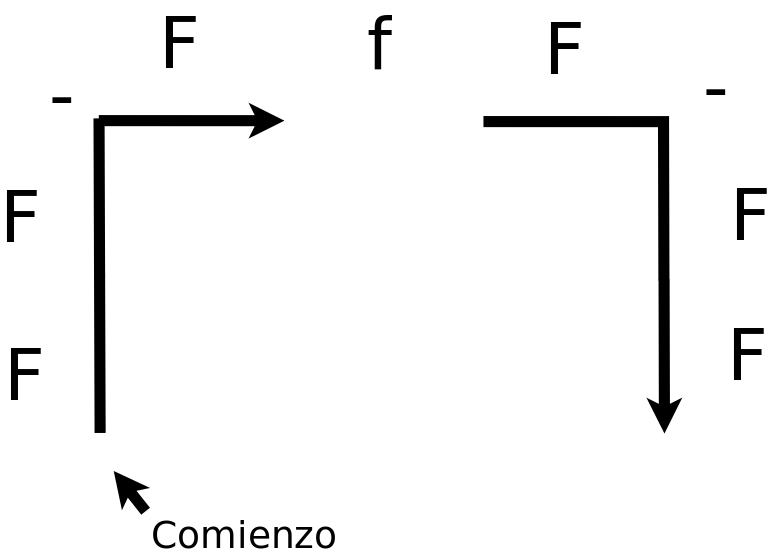
\includegraphics[width=8cm]{figures/tortuga}
\caption{Resultado de la interpretación de tortuga de una cadena de caracteres.}
\label{fg:tortuga}
\end{figure}

La Fig.~\ref{fg:sistemasL} muestra otros ejemplos de sistemas-L, en los cuales se puede observar que con pocas reglas es posible obtener estructuras complejas y de gran belleza.

Usualmente, y debido a la utlización de recursión y repetición, estos sistemas dan lugar a figuras fractales (similares a distintas escalas), por lo cual se las utiliza para dibujar este tipo de estructuras.

\begin{figure}
\center
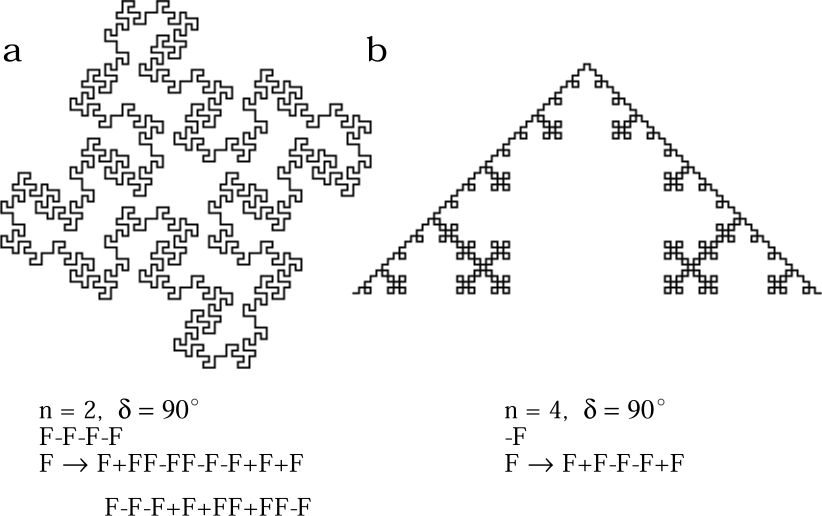
\includegraphics[width=13cm]{figures/sistemasL}
\caption[Sistemas-L generados utilizando distintos parámetros]{Sistemas-L generados utilizando distintos parámetros y una única regla de producción. $n$ es la cantidad de derivaciones utilizadas para producir la cadena que da origen a la figura. En (a), el axioma es F-F-F-F, mientras que en (b) es -F.}
\label{fg:sistemasL}
\end{figure}

Para lograr una imagen que semeje la estructura de árboles y plantas, es necesario introducir dos nuevos caracteres, los cuales son utilizados para generar estructuras ramificadas.
Utilizando una {\em pila} de estados, es posible alcanzar este comportamiento.

El caracter $[$ se utiliza para copiar el estado actual en la pila (operación {\em push}).
De manera análoga, el caracter $[$ implica un reemplazo del estado actual por el de la cabeza de la pila ({\em pop}).
El estado actual de la tortuga está representado por la tripleta antes mencionada.
Por lo tanto, al realizar la operación $]$, en general la posición y orientación de la tortuga serán modificadas.
La utilización de un par $[\dots]$ produce que la tortuga dibuje una rama y vuelva al punto inicial, permitiendo continuar con la computación de otras partes de la estructura.

La Fig.~\ref{fg:sistemasLcorchete} muestra ejemplos de gramáticas que producen geometrías visualmente muy similares a plantas.
Por medio de una única regla de producción es posible obtener distintas plantas, y por medio del número de iteraciones se controla cuánto detalle se producirá en la planta (a mayor número de iteraciones, mayor detalle).

\begin{figure}
\center
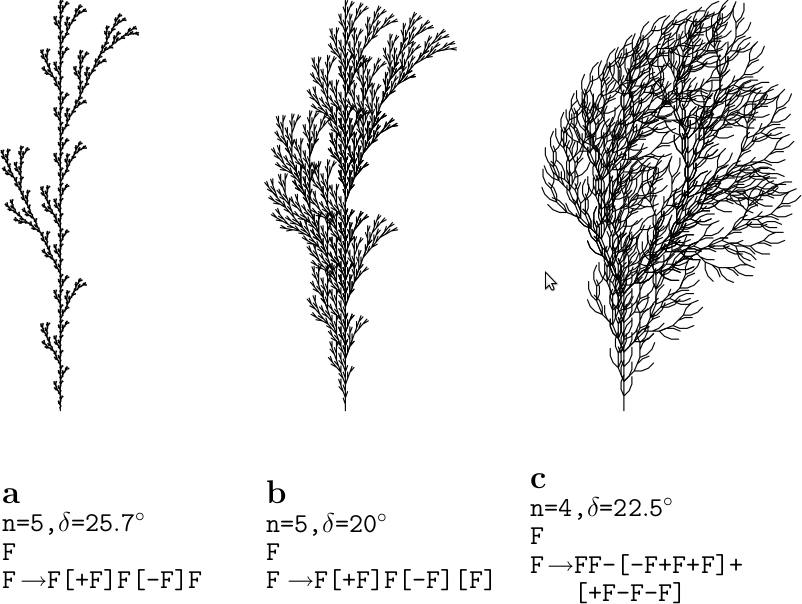
\includegraphics[width=11cm]{figures/sistemalcorchete}
\caption[Sistemas-L con pila de estados, utilizando distintos parámetros]{Sistemas-L con pila de estados, utilizando distintos parámetros. Las imágenes muestran estructuras muy parecidas a plantas. $n$ es la cantidad de derivaciones utilizadas para producir la cadena que da origen a la figura.}
\label{fg:sistemasLcorchete}
\end{figure}


Debido a la facilidad de diseño de nuevas estrategias, y a la naturaleza fenomenológica del método, se han desarrollado numerosas variantes a estos sistemas, los cuales intentan capturar características como mayor aleatoriedad, la aparición de hojas, flores, etc.
Por ejemplo, podría diseñarse una flor como un conjunto de líneas con forma de estrella, y encapsularse a las mismas en una producción de la gramática.
Cuando se desea que se vea una flor, se aplica esta regla.


Entre las especializaciones encontramos sistemas-L estocásticos, los cuales eligen reglas de reescritura de acuerdo a una probabilidad asignada a cada regla, sistemas-L paramétricos, los cuales varían el ángulo y el paso a dibujar dependiendo de la posición de la cadena donde se encuentran, entre otros.
Además, el método se generaliza fácilmente a tres dimensiones, ver Fig.~\ref{fg:sistemasL3D}.
La generalización se realiza por medio de la utilización de matrices de rotación, con un número agregado de operaciones de giro, ver \cite{Prusinkiewicz1990} para obtener mayores detalles.

\begin{figure}
\center
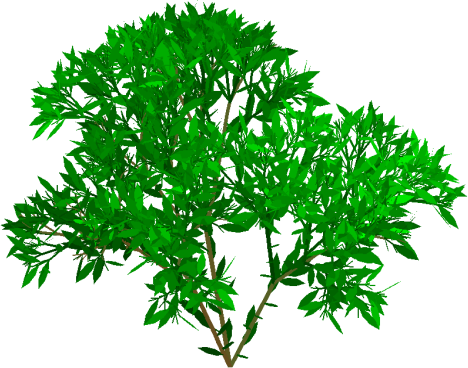
\includegraphics[width=11cm]{figures/3dlsystem}
\caption[Sistema-L en tres dimensiones.]{Planta generada por un sistema-L en tres dimensiones.}
\label{fg:sistemasL3D}
\end{figure}

\subsection{Edificios y Ciudades}
Como fue comentado, una de las ventajas del modelado procedimental está dada por la capacidad de realizar el proceso automáticamente, ahorrando costos y tiempos de diseño.
Un modelado procedimental de edificios puede observarse en \cite{Wonka2003}.
Dicho trabajo presenta un proceso automático que genera de manera casi instantánea edificios arquitectónicamente coherentes, es decir, con ciertas características estructurales que deben ser respetadas.

La principal diferencia en la utilización de sistemas-L en el modelado de edificios, proviene de asumir que un sistema-L constituye una estructura que crece con el tiempo.
Sin embargo, los edificios deben modelarse como conjuntos de objetos con una disposición estática específica.
Para lograr esto, en \cite{Wonka2003} se proponen varias definiciones, entre las que se encuentran gramáticas de división y gramáticas de control.

Una gramática puede ser definida de manera general como un álgebra de objetos $(U,+,-,F,\leq)$, cerrada bajo las operaciones $+$ y $-$, junto a un conjunto de operaciones $F$, de tal forma que si $u$ y $v$ son miembros de $U$, entonces $u+f(v)$ y $u-f(v)$ lo son, donde $f \in F$.

Una gramática $G=(N,T,R,I)$ se define como una tupla de cuatro elementos, donde $N \subset U$ representa los nodos no terminales (es decir que se pueden seguir realizando divisiones), $T \subset U$ los terminales (no se pueden dividir), $I \subset N$ un conjunto de objetos iniciales y $R \subseteq U \times U$ un conjunto de producciones.

%Para comprender mejor estos conceptos, definimos una gramática de conjuntos.
%Este tipo de gramáticas 


Una {\em forma} se define como un conjunto de líneas rectas en el espacio.
Las gramáticas de división seleccionan reglas para subdividir formas en formas más básicas (cubos, cilindros, etc.).

La Fig.~\ref{fg:splitgrammar} muestra un ejemplo del proceso involucrado en una gramática {\em de división}, en la cual una {\em forma} se divide en otras, utilizando reglas definidas por dicha gramática, en este caso formando una secuencia de ventanas.
Como puede observarse, una gramática de este tipo divide de forma completa el espacio de cada forma, en sub-formas de la misma.

Un {\em diseño} final emerge al finalizar el proceso, es decir, en el momento que no existen nodos no terminales ($N$) en la derivación.
La principal diferencia con los sistemas-L se basa en que en aquellos, las reescrituras no necesariamente ocupaban el mismo volumen, como sí debe ocurrir en estas gramáticas.

\begin{figure}
\center
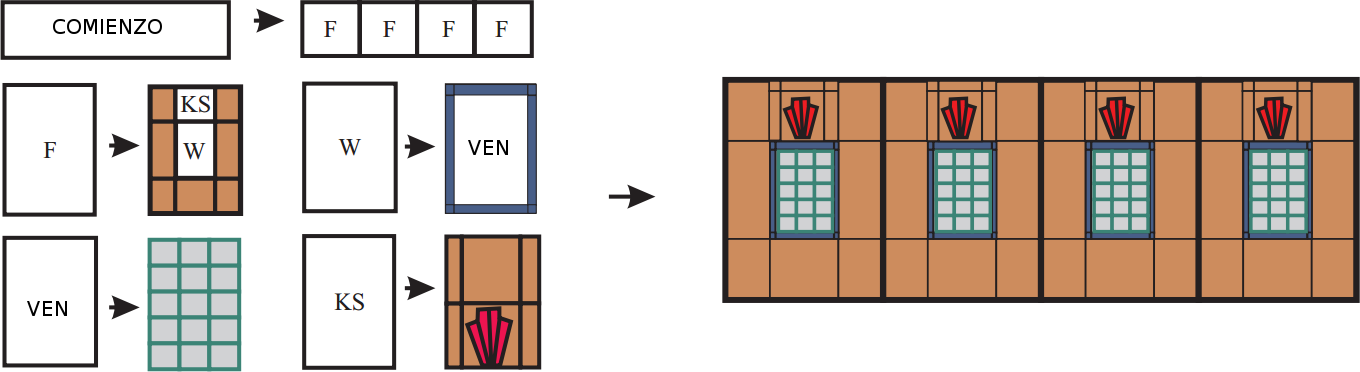
\includegraphics[width=13cm]{figures/splitgrammar}
\caption[Gramática para formar una secuencia de ventanas]{Gramática de división mostrando los pasos seguidos para formar una secuencia de ventanas.}
\label{fg:splitgrammar}
\end{figure}

Las texturas, colores y otras decisiones pueden controlarse por medio de {\em atributos}.
Estos resultan útiles para mantener la coherencia en un mismo piso, por ejemplo, o asegurar que todas las columnas del edificio seguirán un mismo diseño arquitectónico.
Cada símbolo de la gramática se aumenta con uno o más atributos, los cuales especifican estas características para cada parte de la geometría.


Las {\em gramáticas de control} permiten obtener control sobre la distribución de los atributos, y tomar decisiones de diferenciación sobre las divisiones, generando aleatoriedad en los edificios resultantes.
Por ejemplo, se puede requerir que la apariencia del primer piso de un edificio sea diferente al resto (por ejemplo el color, o que sean visibles negocios en la fachada).

Estas gramáticas se invocan a partir de una división específica en una gramática de división.
Cuando se invocan, las mismas generan una secuencia nodos terminales con atributos en la forma $(c,a,v)$, donde $c$ es la posición en la división (fila, columna, capa, en $3D$), $a$ es el atributo y $v$ el valor que tomará.
Estos nodos terminales se utilizan para rellenar los valores de los atributos de las nuevas formas en la división.
Entonces, con una gramática de control se posibilita el control del proceso de distribución de atributos.
Un ejemplo sería asignar el atributo {\em puerta} con $1$ a alguna región de la planta baja, y $0$ al resto del edificio.
De igual modo, pueden controlarse los colores de cada piso, seteando por ejemplo colores distintos de manera alternada.
La Fig.~\ref{fg:controlgrammar} muestra un ejemplo de una gramática de control.


Las gramáticas de control también cumplen el propósito de lograr una distribución correcta de las formas.
Por medio de ellas, también es posible {\em excluir} elementos de ciertas posiciones indeseadas (por ejemplo una columna en el último piso), utilizando los mismos atributos para elegir determinadas reglas por sobre otras, logrando un balance de formas en los resultados finales.

El último paso del procedimiento de síntesis renderiza la representación, donde una gramática con nodos terminales y atributos se interpreta para generar la imagen del edificio.
Esta interpretación depende de los atributos especificados y puede variar de acuerdo a las necesidades de la aplicación.

\begin{figure}
\center
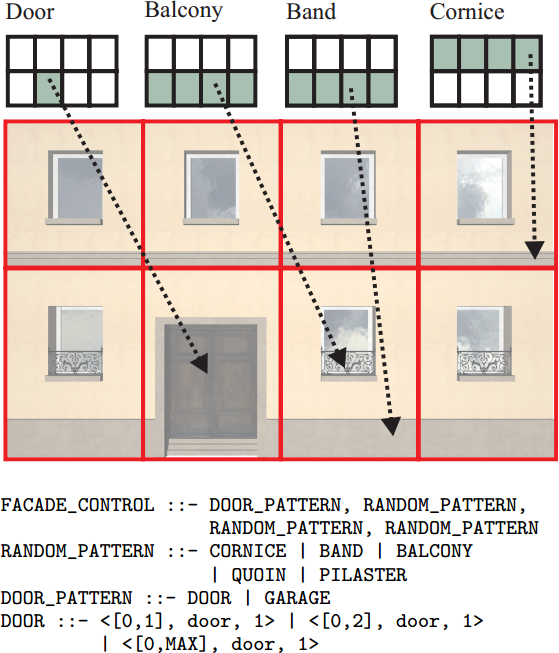
\includegraphics[width=11cm]{figures/controlgrammar}
\caption{Gramática de control.}
\label{fg:controlgrammar}
\end{figure}

La literatura de modelado procedimental de edificios y ciudades ha ido creciendo en los últimos años \cite{Parish2001,Muller2006}.
La Fig.~\ref{fg:edificios} muestra ejemplos de edificios generados procedimentalmente.


\begin{figure}
\center
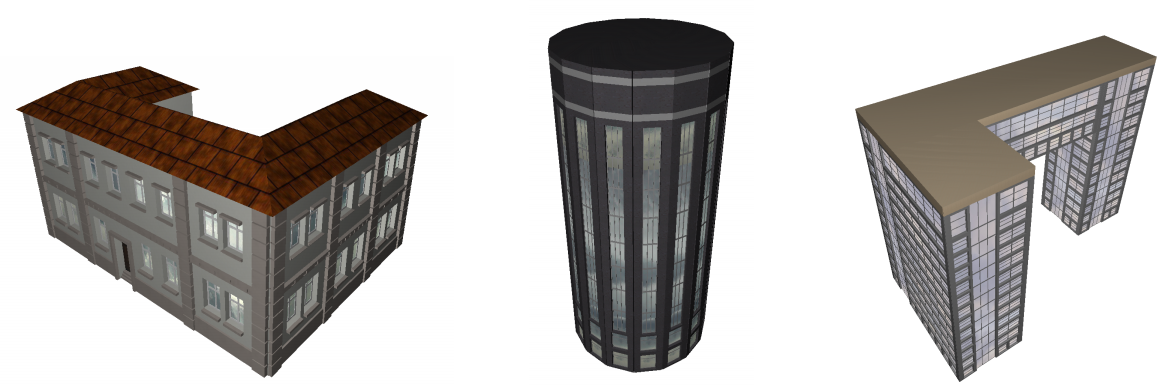
\includegraphics[width=11cm]{figures/edificios}
\caption{Edificios generados procedimentalmente por medio de gramáticas.}
\label{fg:edificios}
\end{figure}

\subsection{Fractales y Montañas}
Una forma adecuada para modelar fenómenos de apariencia pseudo-aleatoria (montañas, ríos, nubes) se da a través de algoritmos fractales \cite{Mandelbrot1983}.
Al igual que en las secciones anteriores, una única fórmula matemática encapsula en una representación suficientemente descriptiva todos los detalles, a diferentes escalas, de un fenómeno u objeto dado.
Esto resulta de particular interés en computación, donde los recursos de memoria no son infinitos.

En el siglo $XIX$, el botánico Robert Brown describió el movimiento de partículas de polen en suspensión en agua, a lo cual se le otorgó el nombre de movimiento browniano.
Los movimientos de la partícula se dan sobre direcciones aleatorias por un período de tiempo también aleatorio.
Con el paso de los años se descubrió que la aparente aleatoriedad de los movimientos responde al choque de la partícula de polen con moléculas dispersas en el agua.
Se asume que los movimientos de la partícula de polen son independientes entre sí.

En \cite{Mandelbrot1968}, se plantea una generalización del método llamada movimiento browniano fraccionario (\acrshort{fBm}). 

\begin{align*}
B_{H}(0,w) &= b_{0},\\
B_{H}(u,w)- B_{H}(0,w) &= \frac{1}{\Gamma(H+0.5)} \big\{ \int_{-\infty}^{u} [(u-s)^{H-0.5} - (-s)^{H-0.5} ] dB(s,w) + \\
&  \int_{0}^{u} (u-s)^{H-0.5} dB(s,w) \big \},
\end{align*}


donde $b_{0}$ es un número real, $0 < H < 1$ es el coeficiente de Hurst, $-\infty < u < \infty $ y $w$ es un conjunto de valores aleatorios en un espacio uniforme de muestras.

Cuando $H = 0.5$ se obtiene movimiento Browniano convencional.
En el dominio frecuencial (al cual se puede acceder por medio de una transformada de Fourier), se observa que el fBm no posee una frecuencia dominante, es decir, la función está compuesta por frecuencias a todas las escalas.
Además, la contribución de cada frecuencia es inversamente proporcional a la misma, es decir que el ruido pertenece a la clase de ruidos $\frac{1}{f}$.
El ruido presenta autosimilaridad estadística.
Intuitivamente significa que las características estadísticas del ruido son similares para todas las escalas.

El ruido resulta ser un fractal no determinístico con dimensión $2-H$.
El parámetro $H$ permite simular perfiles con distintas rugosidades.
Cuando $H = 0$, el ruido es indistinguible de un plano.
Cuando $H = 1$, el ruido se transforma en una línea.
Esto resulta útil para modelar perfiles de montañas con distintas rugosidades (más suaves o más pronunciadas), ver Fig.~\ref{fg:hurst}.

\begin{figure}
\center
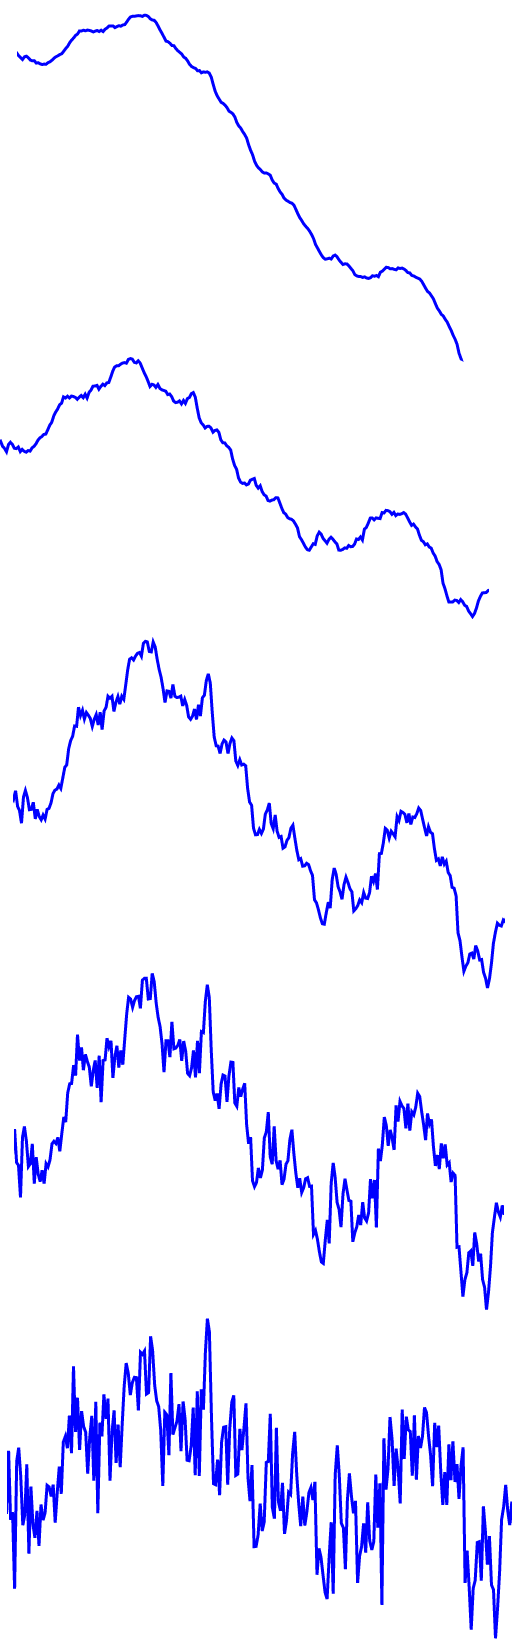
\includegraphics[width=11cm]{figures/hurst}
\caption{Curvas obtenida con distintos coeficientes de Hurst.}
\label{fg:hurst}
\end{figure}

Existen diversos métodos para computar el fBm en computación gráfica.
En \cite{Fournier1982} se presenta un método de subdivisión recursiva, denominado algoritmo de desplazamiento aleatorio del punto medio.

El algoritmo tiene su base en una fórmula de esperanza condicional para $B_{H}(u,w)$ \cite{Mandelbrot1968}.
Partiendo de $B_{H}(0,w) = 0$ y $B_{H}(1,w) = 1$, $0 \le u \le 1$ entonces $E[B_{H}(u,w)|B_{H}(1,w)] = \frac{1}{2} (u^{2H} + 1 - |u-1|^{2H})$.
Si $u=\frac{1}{2}$, entonces la esperanza es igual a $\frac{1}{2}$, independientemente de $H$.
Esto, junto a la autosimilaridad del proceso, permite diseñar un algoritmo que subdivide el segmento en su punto medio, y al valor esperado para el punto medio lo desplaza por un número aleatorio con media $0$ y variancia $1$ multiplicado por la variancia de $B_{H}(u,w)$ en el punto, la cual resulta igual a $2^{-H}$, en términos matemáticos, $2^{-H} * gauss(0,1) $.
Una vez computado el punto medio, el intervalo se subdivide y se computan de manera recursiva las mitades resultantes, donde la nueva variancia será proporcional al tamaño del nuevo segmento.

En la Fig.~\ref{fg:puntomedio} puede observarse un ejemplo de una curva obtenida utilizando distintas profundidades en el algoritmo recursivo.
Se observa que se puede obtener mayor detalle a mayor número de iteraciones, donde la curva resultante asemeja visualmente al perfil de una montaña.

\begin{figure}
\center
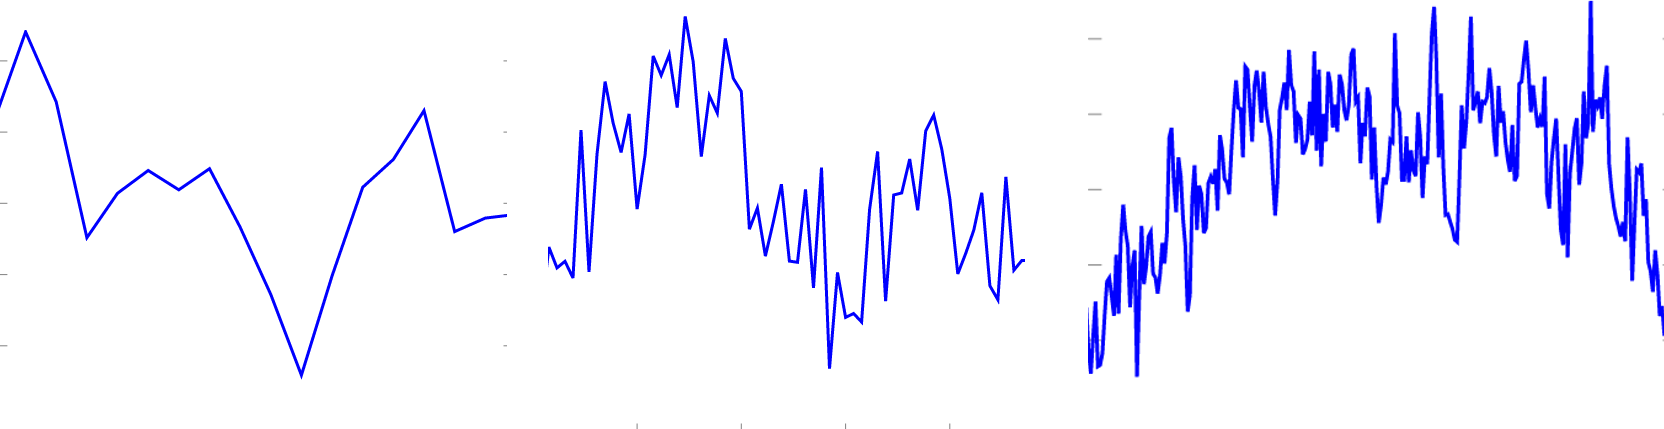
\includegraphics[width=11cm]{figures/puntomedio}
\caption[Curva obtenida utilizando el algoritmo del punto medio]{Curva obtenida con $H=0.8$, para $17$, $65$ y $257$ muestras, utilizando el algoritmo del punto medio.}
\label{fg:puntomedio}
\end{figure}


Una extensión directa de este algoritmo se da en dos dimensiones, donde los valores que se subdividen representan las alturas de un terreno.
Comenzando con $4$ puntos en un plano, formando un cuadrado, donde cada punto almacena la altura del terreno, se puede sudividir el terreno en $4$ cuadrados, a partir de los puntos medios de cada arista del cuadrado original.
$H$ controla la rugosidad del terreno.
La Fig.~\ref{fg:terreno} muestra un ejemplo de la renderización de un terreno generado utilizando este método, donde $H = 0.9$, en la Fig.~\ref{fg:terreno2} $H = 0.3$.
Se puede observar que a medida que $H$ crece, el terreno posee una apariencia más {\em suave}.

\begin{figure}
\center
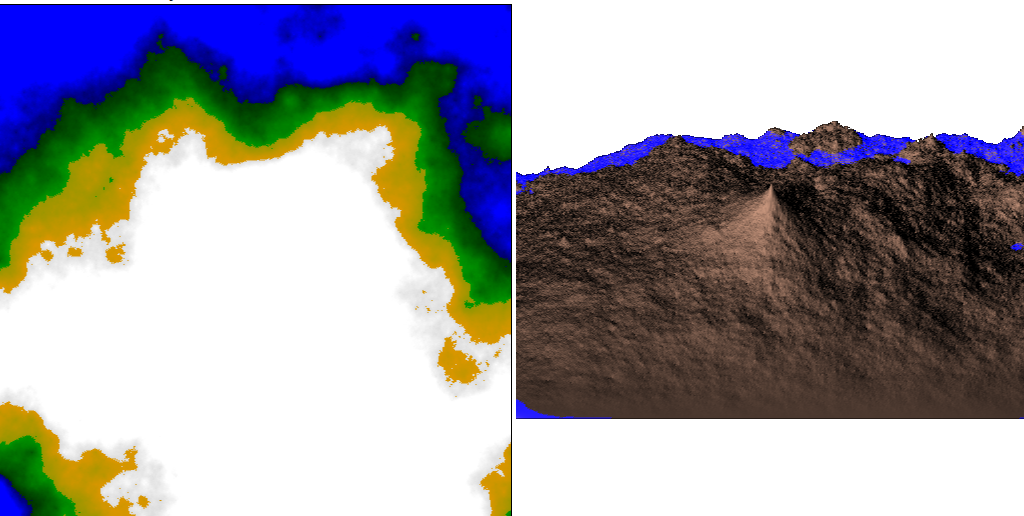
\includegraphics[width=11cm]{figures/terreno}
\caption[Terreno generado utilizando el algoritmo de desplazamiento del punto medio en dos dimensiones, con $H = 0.9$]{Terreno generado utilizando el algoritmo de desplazamiento del punto medio en dos dimensiones, con $H = 0.9$. La imagen de la izquierda muestra colores agregados de acuerdo al número generado, la imagen de la derecha muestra un ejemplo tridimensional de los mismos datos visto en perspectiva.}
\label{fg:terreno}
\end{figure}

\begin{figure}
\center
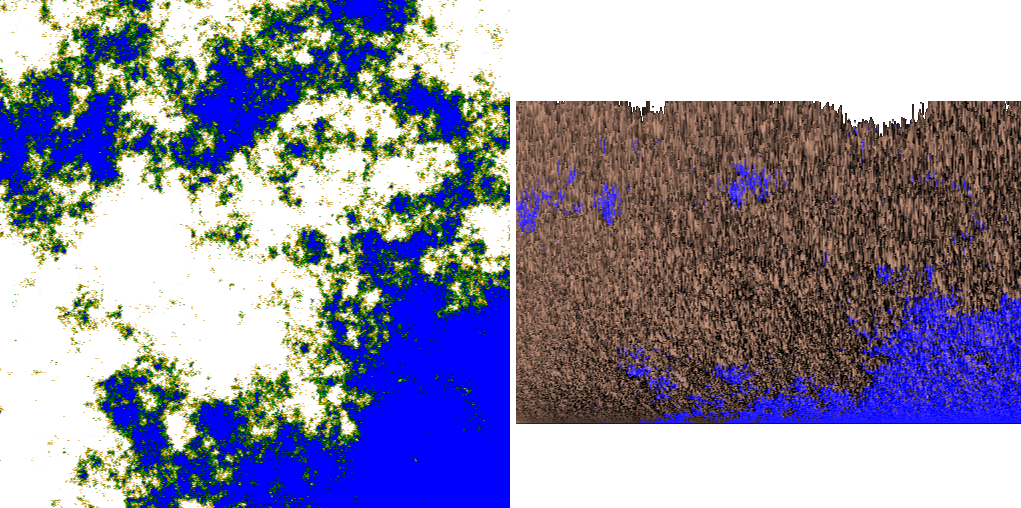
\includegraphics[width=11cm]{figures/terreno2}
\caption[Terreno generado utilizando el algoritmo de desplazamiento del punto medio en dos dimensiones, con $H = 0.3$]{Terreno generado utilizando el algoritmo de desplazamiento del punto medio en dos dimensiones, con $H = 0.3$.}
\label{fg:terreno2}
\end{figure}

%\subsubsection{Planetas}
%\cite{Ebert2002}


\subsection{Modelos Físicos}
Si bien los resultados obtenidos por los modelos presentados hasta ahora son muy satisfactorios, existe aún la necesidad de no depender de parámetros ad-hoc, además de aumentar el realismo de las imágenes resultantes.
Hasta aquí, la utilización de los modelos se basa casi exclusivamente en su {\em parecido visual} a los objetos que se intentan modelar.

Para obtener una representación más ajustada a la geometría real de los materiales, se apela a los procesos físicos de formación o comportamiento de los materiales (movimiento de partículas, deformaciones, reacciones químicas, etc.), lo cual permitiría definir parámetros más intuitivos que tienen su correlación en la realidad, logrando además una representación más exacta de la misma.
La desventaja de utilizar modelos físicos o matemáticos, recae sobre los tiempos de cómputo y la dificultad de diseño de éstos.

Sin embargo, desde el surgimiento del área, estos modelos han ido evolucionando gracias al incremento en el poder de cómputo del hardware gráfico disponible. A pesar de esto, aún nos encontramos en los comienzos de la utilización masiva de los mismos, por lo cual existen sólo unos pocos casos en los que se utilizan modelos de primeros principios.
En esta sección presentamos un ejemplo de esto, lo cual ejemplifica la capacidad de representación que puede alcanzarse al agregar detalles reales en las implementaciones.

\subsection{Fluidos}
Entre los primeros intentos por utilizar procesos físicos para modelar la apariencia de los materiales, encontramos ecuaciones que describen fluidos.
Las ecuaciones de Navier-Stokes describen un fluído con temperatura prácticamente constante, por medio de un campo vectorial de velocidades $\bold{u}$ y un campo de presiones $p$.

Dadas condiciones iniciales para $\bold{u}$ y $p$ cuando $t = 0$, la evolución de las cantidades puede describirse como sigue, independientemente del número de dimensiones,

\begin{align}
\nabla \cdot \bold{u} &= 0, \label{eq:eq1}\\
\frac{\partial \bold{u} }{\partial t} &= - (\bold{u} \cdot \nabla) \bold{u} - \frac{1}{\rho} \nabla p + \nu \nabla^{2} \bold{u} + \bold{f} \label{eq:eq2},
\end{align}

donde $\nu$ representa la viscosidad cinemática del fluído, $\rho$ la densidad y $\bold{f}$ una fuerza externa.
Las ecuaciones modelan la conservación de masa (\ref{eq:eq1}) y de momento (\ref{eq:eq2}).

Además, deben tenerse en cuenta condiciones de borde.
Las mismas pueden variar en complejidad.
Por ejemplo, una implementación sencilla puede darse utilizando condiciones de borde periódicas, es decir, sin la existencia de {\em paredes} (el fluido se repite indefinidamente, condición utilizada en el trabajo descripto aquí).
Un caso más realista lo constituye una condición diferencial que describe el intercambio de masa con el ambiente.

Es posible combinar ambas ecuaciones para obtener una única ecuación de la velocidad.
Para esto, se utiliza la descomposición de Helmholtz-Hodge \cite{Chorin1990}, la cual establece que un campo vectorial $\bold{w}$ puede descomponerse como sigue, 

\begin{equation}
\label{eq:eq3}
\bold{w} = \bold{u} + \nabla q,
\end{equation}

donde $\bold{u}$ tiene divergencia $0$, es decir $\nabla\cdot\bold{u} = 0$.
Entonces, se puede definir un operador $\bold{P}$, el cual proyecta un campo vectorial $\bold{w}$ en su componente de divergencia $0$, $\bold{u} = \bold{P}\bold{w}$.
Dicho operador se puede definir implícitamente multiplicando $\nabla$ en ambos términos en la ecuación (\ref{eq:eq3}),

\begin{equation}
\label{eq:eq4}
\nabla\cdot\bold{w} = \nabla^{2} q.
\end{equation}

Una solución a esta ecuación está dada por

\begin{equation}
\label{eq:eq5}
\bold{u} = \bold{P}\bold{w} = \bold{w} - \nabla q,
\end{equation}

Aplicando el operador $\bold{P}$ en ambos lados de la ecuación (\ref{eq:eq2}), se obtiene una ecuación única para la velocidad,

\begin{equation}
\frac{\partial \bold{u} }{\partial t} = \bold{P} (- (\bold{u} \cdot \nabla) \bold{u} + \nu \nabla^{2} \bold{u} + \bold{f}) \label{eq:eq6},
\end{equation}

ya que $\bold{P}\bold{u} = \bold{u}$ y $\bold{P}\nabla p = 0$.
Esta ecuación se utiliza en la derivación de un algoritmo práctico que implementa apariencia de fluídos \cite{Stam1999}.
En la ecuación pueden verse un paso difusivo $\nu \nabla^{2} \bold{u}$, un paso de advección $- (\bold{u} \cdot \nabla) \bold{u}$ y una fuerza final aplicada $\bold{f}$.
Estos términos pueden resolverse por medio de la aplicación de métodos numéricos clásicos (por ejemplo diferencias finitas), por lo cual la solución final consiste en aplicar sucesivamente cada paso para obtener soluciones al campo vectorial $u$ en cada instante de tiempo $t$, finalmente proyectando el resultado con $P$.
El paso más complicado lo constituye el paso de proyección $P$, el cual se resuelve por medio de sistemas lineales, teniendo en cuenta que la misma constituye una ecuación de Poisson.

Las velocidades $\bold{u}$ permiten definir un sistema de partículas sobre el fluido, otorgando velocidades a las partículas, correspondientes a su localización en el medio.
Luego, las partículas podrán ser renderizadas.

Este método se utiliza para modelar el comportamiento de agua y otros líquidos, además de algunos gases, nubes y humo, ver Figs.~\ref{fg:fluidos1},\ref{fg:fluidos2}.

La utilización de los procesos físicos subyacentes produce mayor realismo en las imágenes resultantes sobre la utilización de métodos heurísticos y fenomenológicos.
Desafortunadamente, muchas veces este enfoque resulta prohibitivo, no solo debido a costos computacionales, sino también por la complejidad presente en el diseño de los métodos, ya que se requiere muchas veces la participación de personas provinientes de áreas científicas afines a la física utilizada.


\begin{figure}
\center
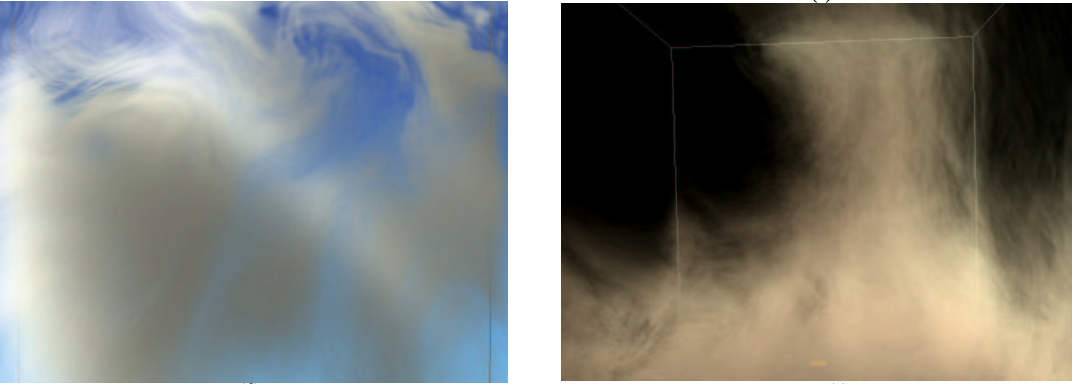
\includegraphics[width=11cm]{figures/fluidos1}
\caption{Nubes y humo generados utilizando métodos basados en las ecuaciones de Navier-Stokes.}
\label{fg:fluidos1}
\end{figure}

\begin{figure}
\center

\includegraphics[width=11cm]{figures/fluidos2}
\caption{Fluidos generados utilizando métodos basados en las ecuaciones de Navier-Stokes.}
\label{fg:fluidos2}
\end{figure}

%\subsubsection{Telas}

\section{Representación Visual (Renderizado)}

Además de presentar una geometría compleja, los materiales exhiben fenómenos particulares en su interacción con la luz, entre los cuales se observan translucencia, reflectancia, absorción, etc.
Cada fenómeno puede determinar de forma inequívoca la apariencia de un material determinado.
Debido a esto, en las décadas posteriores al nacimiento de la informática gráfica, se desarrollaron distintas técnicas, inpiradas en determinadas ecuaciones físicas que fueron simplificadas y aproximadas para ser implementadas por medio de una computadora, permitiendo modelar la apariencia de una gran variedad de materiales.

\subsection{Ecuación del Renderizado}

Esta ecuación modela el comportamiento de la luz en una escena y su interacción con distintos tipos de superficies \cite{Kajiya1986}.
La misma se basa en el principio de la conservación de la energía, el cual establece que la energía saliente debe ser igual a la energía entrante, más la energía emitida, menos la energía absorbida.
La ecuación presenta la siguiente definición:

\begin{equation}
L(\bold{x'} \rightarrow \bold{x}) =  g(\bold{x'}  \rightarrow \bold{x})  \left[ \epsilon(\bold{x'}  \rightarrow \bold{x}) + \int_{s}{\rho(\bold{x''}  \rightarrow \bold{x'}  \rightarrow \bold{x})L(\bold{x''}  \rightarrow \bold{x}) d\bold{x''}} \right],
\end{equation}
donde $L(\bold{x'} \rightarrow \bold{x})$ representa la intensidad de la luz que viaja del punto tridimensional $\bold{x'}$ al punto $\bold{x}$ (sin oclusiones), $g(\bold{x'} \rightarrow \bold{x})$ un termino geométrico que modela la oclusión que podría existir entre $\bold{x}$ y $\bold{x'}$, $\epsilon(\bold{x'} \rightarrow \bold{x})$ la intensidad de la luz emitida desde $\bold{x'}$ a $\bold{x}$, $\rho(\bold{x''}  \rightarrow \bold{x'}  \rightarrow \bold{x})$ la intensidad de la luz emitida de $\bold{x''}$ a $\bold{x}$ por medio de una superficie en $\bold{x'}$ (esta cantidad será llamada función bidireccional de distribución de reflectancia, \acrshort{BRDF}, en una sección posterior), y $S=\bigcup{s_{i}}$ la unión de todas las superficies $s_{i}$ de la escena.


Puede observarse que la ecuación presenta una definición recursiva, ya que la energía radiante saliente de un punto $x'$ depende de la energía radiante que llega desde todos los puntos de todas las superficies a ese punto.
De esta forma, $\bold{x}$,$\bold{x'}$ y $\bold{x''}$ varían sobre todas las superficies de la escena.
Además se asume una superficie $S_{0}$, la cual se modela como un semi-hemisferio que engloba a toda la escena.

La ecuación aproxima las propiedades óptico-geométricas de las ecuaciones del electromagnetismo de Maxwell.
$L$ representa la radiación de energía por unidad de tiempo por unidad de superficie de destino por unidad de superficie de origen ($joule/m^{4} s$).
El término geométrico resulta $0$ si los puntos en consideración no son mutuamente visibles.

El modelado de cada término, separadamente, posibilita la visualización fiel de una gran cantidad de superficies.
Trabajos previos a la aparición de la ecuación del renderizado alcanzaron resultados parciales, sin lograr sintetizar un único método que englobe todos los fenómenos en investigación hasta ese entonces.
Entre los casos particulares de la ecuación del renderizado, los más emblemáticos han sido el trazado de rayos \cite{Whitted1980} y la radiosidad \cite{Goral1984}.
El primero resulta adecuado para renderizar superficies especulares (la luz se refleja en las superficies en direcciones específicas), mientras que la radiosidad resulta idónea para simular superficies cuyas geometrías microscópicas provocan una distribución de la luz reflejada de manera equitativa, produciendo una apariencia difusa.

Fuera de la ecuación quedan efectos más complejos, como la difracción y la polarización.
Más detalles de la misma pueden ser consultados en \cite{Kajiya1986}.
Un esquema de esta ecuación puede observarse en la Fig. \ref{fg:rendequation}.

\begin{figure}
\center
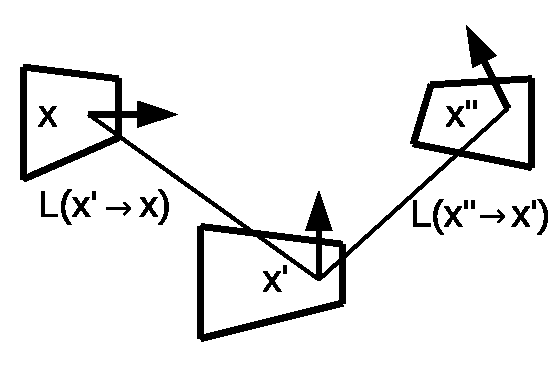
\includegraphics[width=8cm]{figures/rendequation}
\caption[Interpretación visual de la ecuación del renderizado]{Interpretación visual de la ecuación del renderizado (término $L(\bold{x''}  \rightarrow \bold{x}) $). La ecuación modela la distribución de radiancia en una escena, considerando todas las superficies intervinientes. La imagen muestra además los vectores normales a las superficies.}
\label{fg:rendequation}
\end{figure}

La ecuación presentada modela correctamente el comportamiento de la energía radiante en superficies en una escena tridimensional.
Si lo que se pretende modelar son fenómenos volumétricos, como partículas en el ambiente, o materiales transparentes, entre otros ejemplos, entonces deben atenderse ciertas generalizaciones de la ecuación, como se desarrolla en la siguiente sub-sección.

\subsection{Ecuación del Renderizado de Volúmenes}

En esta sección denotaremos como $L(\bold{x} \rightarrow \vec{\omega})$ a la energía radiante o {\em radiancia} que parte desde un punto del espacio $\bold{x}$ en la dirección $\vec{\omega}$.
Siguiendo la notación de la sección anterior, para cada vector en el espacio $\vec{\omega}$, existe un punto tridimensional $\bold{y}$ tal que $L(\bold{x} \rightarrow \vec{\omega}) = L(\bold{x} \rightarrow \bold{y})$.

La luz se modeliza por medio de partículas denominadas {\em fotones}. Cuando un fotón de un rayo de luz atraviesa un medio en una dirección dada, pueden ocurrir una serie de eventos, de los cuales dos corresponden a fenómenos de extinción: la absorción y la redirección del mismo en otra dirección.
Estos fenómenos dependen del coeficiente de absorción del medio $\sigma_{a}$ y el coeficiente de dispersión $\sigma_{s}$.
La suma de ambos se denota como el coeficiente de extinción $\sigma_{t}$.

El coeficiente de absorción en un segmento de recta se denota como $\sigma_{a}(\bold{x} + t\vec{\omega})$.
La fracción de fotones absorbidos en ese segmento de recta se nota como $\sigma_{a}(\bold{x} + t\vec{\omega}) \Delta t$.
Consecuentemente la fracción de fotones que escapa a la absorción en ese segmento de recta resulta $(1-\sigma_{a}(\bold{x} + t\vec{\omega}) \Delta t)$.
Finalmente, podemos escribir la radiancia que {\em escapa} del medio en dirección $\vec{\omega}$ como,

$$L((\bold{x}+t\vec{\omega}) \rightarrow \vec{\omega}) = L(\bold{x} \rightarrow \vec{\omega}) (1-\sigma_{a}(\bold{x} + t\vec{\omega}) \Delta t),$$

o, de otra forma:

$$\frac{L((\bold{x}+t\vec{\omega}) \rightarrow \vec{\omega}) - L(\bold{x} \rightarrow \vec{\omega}) }{ \Delta t } = - \sigma_{a}(\bold{x} + t\vec{\omega}) L(\bold{x} \rightarrow \vec{\omega}).$$

Tomando el límite cuando $\Delta t \rightarrow 0$ se obtiene la derivada, es decir, el cambio diferencial en radiancia dado por la absorción del medio,

$$\lim_{\Delta t \rightarrow 0} \frac{L((\bold{x}+t\vec{\omega}) \rightarrow \vec{\omega}) - L(\bold{x} \rightarrow \vec{\omega}) }{ \Delta t } = (\vec{\omega} \cdot \nabla_{a}) L(\bold{x} \rightarrow \vec{\omega}) = - \sigma_{a}(\bold{x}) L(\bold{x} \rightarrow \vec{\omega}),$$

donde $\nabla_{a}$ denota el gradiente dado por la absorción y $ \vec{\omega} \cdot \nabla_{a}$ expresa la derivada direccional de la absorción del medio en dirección $\vec{\omega}$.

Similarmente se halla el cambio en radiancia debido a la dispersión saliente,

$$ (\vec{\omega} \cdot \nabla_{o}) L(\bold{x} \rightarrow \vec{\omega}) = -\sigma_{s}(\bold{x}) L(\bold{x} \rightarrow \vec{\omega}),$$

de esta forma se pueden aunar ambos términos para expresar el cambio en radiancia debido a la extinción,

$$(\vec{\omega} \cdot \nabla_{t}) L(\bold{x} \rightarrow \vec{\omega}) = -(\sigma_{a}(\bold{x})+\sigma_{s}(\bold{x})) L(\bold{x} \rightarrow \vec{\omega}) = -\sigma_{t}(\bold{x}) L(\bold{x} \rightarrow \vec{\omega}).$$

Gracias a esta expresión se puede calcular una cantidad de interés, llamada {\em Transmitancia}, $T_{r}$, la cual describe la cantidad de fotones que pueden viajar sin obstrucciones entre dos puntos en un medio (en línea recta).
La integración de la ecuación anterior permite obtener una expresión para la transmitancia,

$$T_{r}(\bold{x'} \leftrightarrow \bold{x}) = e^{-\tau(\bold{x'} \leftrightarrow \bold{x})},$$

donde $\tau$ recibe el nombre de densidad óptica del material y su expresión es,

$$\tau(\bold{x'} \leftrightarrow \bold{x}) = \int_{0}^{d} -\sigma_{t}(\bold{x}+t\vec{\omega})dt,$$

con $t \in [0,d]$.
La ecuación resulta de integrar la extinción a lo largo del segmento de recta.


Hasta ahora se describió la pérdida de fotones a medida que un rayo de luz viaja por un medio.
Similarmente existen dos fenómenos que provocan el desvío de fotones hacia la dirección $\vec{\omega}$.
El primero lo constituye la dispersión entrante, fenómenos que provocan una modificación en la dirección de fotones por la del rayo actual.
Su expresión matemática es

$$ (\vec{\omega} \cdot \nabla_{i}) L(\bold{x} \rightarrow \vec{\omega}) = \sigma_{s}(\bold{x}) L_{i}(\bold{x} \rightarrow \vec{\omega}).$$

El último fenómeno ocurre en medios que transforman otras formas de energía como el calor, en luz visible, y se llama emisión, con expresión

$$ (\vec{\omega} \cdot \nabla_{e}) L(\bold{x} \rightarrow \vec{\omega}) = \sigma_{a}(\bold{x}) L_{e}(\bold{x} \rightarrow \vec{\omega}).$$

La ecuación en su forma completa representa el comportamiento de la luz en volúmenes, considerando los cuatro fenómenos \cite{Jarosz2008}:

\begin{equation}
\begin{aligned}
(\vec{\omega} \cdot \nabla) L(\bold{x} \rightarrow \vec{\omega}) = - \sigma_{a}(\bold{x}) L(\bold{x} \rightarrow \vec{\omega}) - \sigma_{s}(\bold{x}) L(\bold{x} \rightarrow \vec{\omega}) + \\
\sigma_{a}(\bold{x}) L_{e}(\bold{x} \rightarrow \vec{\omega}) + \sigma_{s}(\bold{x}) L_{i}(\bold{x} \rightarrow \vec{\omega}).
\end{aligned}
\end{equation}

La misma expresa que el cambio ($\nabla$) de radiancia $L$ de un rayo de luz en un medio, en una dirección dada ($\vec{\omega}$) está dado por cuatro fenómenos: absorción, dispersión saliente, emisión (del medio) y dispersión entrante, ver Fig.~\ref{fg:fenomenosrte}.
Esta ecuación recibe el nombre de ecuación del transporte radiativo (Radiative Transport Equation, \acrshort{RTE}) \cite{Chandrasekhar1960}.

Podemos expresar esta ecuación en forma integral integrando ambos lados de la igualdad, y asumiendo como condición de borde a la ecuación del renderizado de la sección anterior, obteniendo,

\begin{equation}
\begin{aligned}
L(\bold{x} \leftarrow \vec{\omega}) = T_{r}(\bold{x} \leftrightarrow \bold{x_{s}}) L(\bold{x_{s}} \rightarrow -\vec{\omega}) + \\
\int_{0}^{s}{T_{r}(\bold{x} \leftrightarrow \bold{x_{t}}) \sigma_{a}(\bold{x}) L_{e}(x \rightarrow -\vec{\omega}) dt } + \\
\int_{0}^{s}{T_{r}(\bold{x} \leftrightarrow \bold{x_{t}}) \sigma_{a}(\bold{x_{t}}) L_{i}(x_{t} \rightarrow -\vec{\omega})  }
\end{aligned}
\label{eq:rteintegral}
\end{equation}

donde $L(\bold{x} \leftarrow \vec{\omega})$ describe la radiancia que llega a $\bold{x}$ desde $\bold{\omega}$ (este constituye el caso inverso a $L(\bold{x} \rightarrow {\vec{\omega}})$, el cual resulta útil en el diseño de algoritmos que implementan esta ecuación), $s$ es la profundidad del medio desde $\bold{x}$ en dirección $\vec{\omega}$, $\bold{x_{t}} = \bold{x} + t\vec{\omega}$ con $t \in (0,s)$ y $\bold{x_{s}} = \bold{x}+ s\vec{\omega}$ es un punto en una superficie cercana y visible desde el medio, ver Fig.~\ref{fg:rte}.
El primer término de la ecuación representa radiancia entrando por detrás del medio.
El segundo, la emisión de radiancia en el medio.
El último, la acumulación de radiancia entrante al medio. 
Esta forma integral de la ecuación RTE recibe el nombre {\em Ecuación del Renderizado de Volúmenes}.

Esta ecuación resulta aún más compleja que la ecuación del renderizado presentada en la sección anterior.
Cada punto del medio depende de {\em todos} los demás puntos del medio, por lo que deben desarrollarse métodos que permitan computar aproximaciones adecuadas de la misma.
Simplificaciones usuales incluyen ignorar el término de emisión, y asumir un medio isotrópico u homogéneo.

Como fue aclarado, diversos algoritmos específicos surgieron con anterioridad a estas ecuaciones generales, y sin saberlo, formaban parte de un mismo marco teórico, las cuales hoy por hoy son algoritmos especializados para ciertos tipos de materiales y situaciones.



\begin{figure}
\center
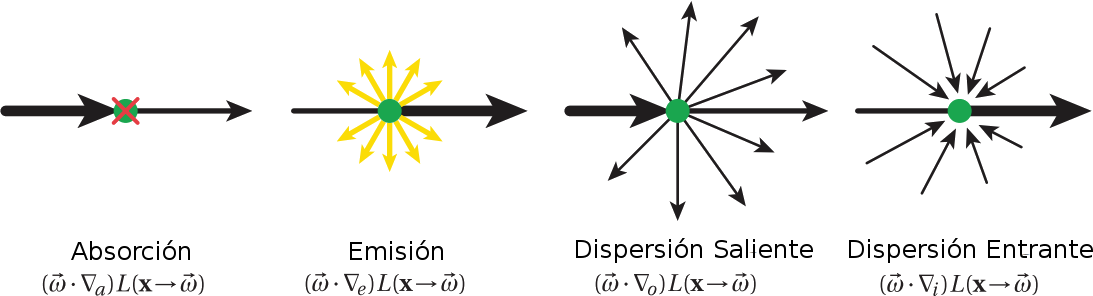
\includegraphics[width=11cm]{figures/fenomenosrte}
\caption{Fenómenos intervinientes en la Ecuación del Transporte Radiativo.}
\label{fg:fenomenosrte}
\end{figure}

\begin{figure}
\center
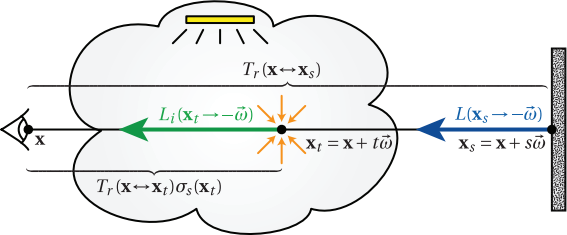
\includegraphics[width=11cm]{figures/rte}
\caption{Interpretación gráfica de la Ecuación del Transporte Radiativo.}
\label{fg:rte}
\end{figure}


%\section{Simplificaciones a las Ecuaciones de Renderizado}
\section{Funciones de Distribución de Reflectancia (BRDFs)}
En la ecuación del renderizado se introdujo un término llamado BRDF, el cual representa una función que modela el comportamiento de la luz en relación con una superficie determinada.
Dada una dirección de entrada y una de salida de un rayo de luz que impacta una superficie, la función devuelve la cantidad de radiancia que emite la superficie en la dirección saliente al recibir energía radiante en su dirección entrante.

\begin{figure}
\center
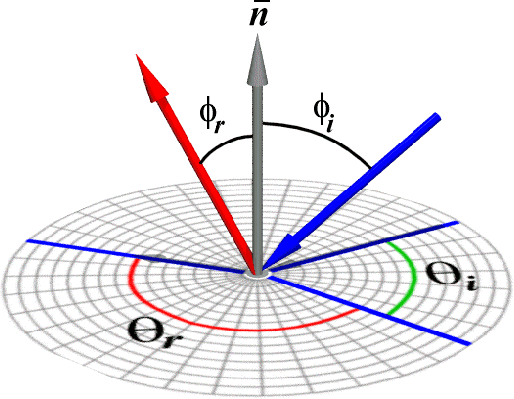
\includegraphics[width=9cm]{figures/brdf}
\caption[Esquema gráfico de la función bidireccional de distribución de reflectancia]{Esquema gráfico de la función bidireccional de distribución de reflectancia (BRDF). El par de ángulos de entrada ($\theta_{i},\phi_{i}$) define la dirección del rayo entrante, similarmente ($\theta_{r},\phi_{r}$) representan la dirección del rayo saliente. La función calcula la cantidad de radiancia emitida en la dirección del rayo saliente, a partir de la dirección del rayo entrante.}
\label{fg:brdf}
\end{figure}

Diversos fenómenos tienen lugar cuando un rayo de luz impacta una superficie de un objeto. En su máxima expresión, una BRDF podría tomar en consideración variables como la longitud de onda, la posición de salida del rayo reflejado en la superficie (modelando de esta forma dispersión interna en el material), e incluso el tiempo de demora entre la entrada y la salida del rayo.
De esta forma sería posible modelar fenómenos tan complejos como la fosforescencia y la polarización.

Una complejidad tal no resulta práctica en computación gráfica, por lo cual deben realizarse simplificaciones sobre los materiales subyacentes.
Una simplificación muy común de esta función consiste en ignorar los fenómenos anteriores y limitar la definición de la BRDF a un par de ángulos de entrada y de salida, para cada punto de la superficie, como se muestra en la Fig. \ref{fg:brdf}.
Esta simplificación resulta en una función de {\em seis} variables, que incluye las cuatro dimensiones definidas por las direcciones de entrada y de salida, y las dos que se corresponden a una representación paramétrica de una superficie.

Debido a la prohibitiva complejidad aún presente en estas simplificaciones, los primeros modelos utilizados en computación gráfica eran funciones analíticas \cite{Phong1975,Blinn1977}, es decir, una función simple que no requería almacenamiento de datos (ya que el valor se calcula en el momento de llamar a la función).
De esta manera fue posible representar diversos materiales sencillos, sobre todo metales y objetos con una marcada reflectancia.
Las funciones no estaban basadas en ningún procedimiento de obtención, sino más bien en un procedimiento artístico que producía resultados aceptables.

Posteriormente surgieron modelos más precisos, los cuales desarrollaron funciones analíticas teniendo en consideración mayores precisiones sobre los modelos geométricos subyacentes, por lo que resultaron más ajustadas a los fenómenos reales \cite{He1991,Ward1992,Lafortune1997}.
Para esto, se modelaron las anisotropías en la reflectancia presentes en las superficies (reflectancia diferente para distintos ángulos).
En otras palabras, la inclusión de no linealidad otorga un mayor realismo.

Otros trabajos \cite{Dana1999,Matusik2003} realizaron mediciones de la reflectancia de materiales por medio de dispositivos de captura (goniorreflectómetros), lo cual constituye una solución de fuerza bruta, pero adecuada en algunos casos.
Los datos de las mediciones del material generalmente son publicados para uso de la comunidad gráfica y científica.

Finalmente, se ha intentado representar los datos mesurados en materiales reales con modelos matemáticos, buscando reducir costos de almacenamiento \cite{Ngan2005}.
En estos casos, por medio de modelos estándar de BRDFs, o por una combinación de los mismos, se buscan explicar los datos obtenidos en las medidas, con lo cual resulta innecesario almacenar la información capturada, computando la misma a partir de la definición del nuevo modelo.
Si bien estas aproximaciones no constituyen modelos de {\em la totalidad} de los datos capturados, generalmente obtienen buenas aproximaciones que emulan gran parte de las observaciones.

\subsection{Definición}
Previamente definimos la BRDF como una función matemática que tomaba como parámetro tres puntos del espacio.
Una forma equivalente consiste en definir, para cada punto de una superficie, el ángulo de entrada y salida del rayo

$$\rho(\theta_{i},\phi_{i},\theta_{r},\phi_{r}) = \frac{dL_{r}(\theta_{r},\phi_{r})}{dE_{i}(\theta_{i},\phi_{i})},$$

donde $E_{i}$ constituye la {\em irradiancia} entrante, definida como flujo incidente sobre unidad de área, y $L_{r}$ nota la radiancia reflejada.
Intuitivamente, la BRDF mide la cantidad de luz reflejada a partir de la cantidad de energía incidente en la superficie, para cada ángulo de entrada y de salida.

Muchas BRDF modelan por separado determinadas características comunes en materiales.
Por ejemplo, las contribuciones especulares (reflejos perfectos) y difusa (la luz se disipa en todas las direcciones de manera equitativa).
La primera produce diferencias visibles en superficies, siendo característica la visualización de círculos o líneas blancas sobre determinadas direcciones en las que se posiciona el observador.

La Fig.~\ref{fg:contribuciones} muestra ejemplos de estos rebotes.
Las direcciones de reflejo suelen formar patrones llamados lóbulos, los cuales permiten entender intuitivamente el comportamiento de la BRDF (se puede predecir las direcciones donde habrá mayor radiancia saliente).
Si el observador se coloca en la dirección de reflejo de estos lóbulos, observará mayor radiancia que en otras direcciones.

\begin{figure}
\center
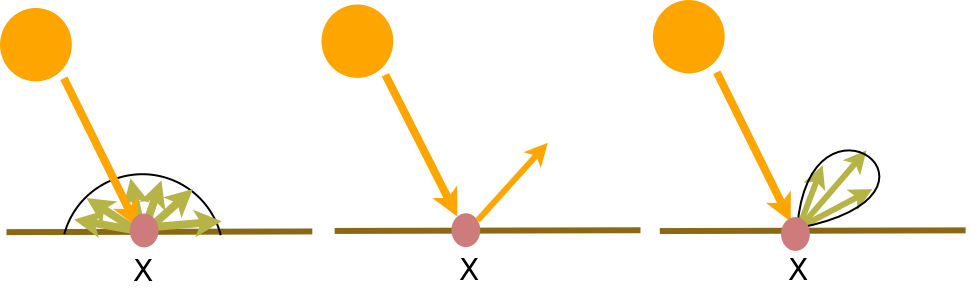
\includegraphics[width=11cm]{figures/contribuciones}
\caption[Diferentes reflectancias en BRDFs]{Diferentes reflectancias en BRDFs. La imagen de la izquierda muestra una reflexión difusa, la del centro, una completamente especular, y la de la derecha, lobular.}
\label{fg:contribuciones}
\end{figure}

La Fig.~\ref{fg:microestructura} muestra un ejemplo de una geometría microscópica de un material y su BRDF resultante.
Como puede observarse, la apariencia final de una BRDF depende de la orientación de determinadas estructuras presentes a escalas microscópicas del material.
En algunos materiales resulta válido asumir distribuciones estadísticas de reflectancia.
Sin embargo, la mayoria de los materiales está constituído de microgeometrías con estructuras en extremo complejas, responsables de marcadas anisotropías en sus patrones de reflectancia.
Como fue discutido, debido a las dificultades presentes en el modelado matemático del comportamiento lumínico en la apariencia de materiales, muchas veces se recurre a mediciones sobre muestras reales.


\begin{figure}
\center
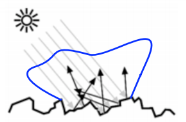
\includegraphics[width=5cm]{figures/microestructura}
\caption{Explicación del comportamiento observable en BRDFs.}
\label{fg:microestructura}
\end{figure}


\subsection{BRDF de Phong}
Un ejemplo muy común de BRDF analítica está dado por el modelo de Phong, ver Fig~\ref{fg:phongVecs}, el cual presenta la siguiente definición matemática:

$$\rho_{phong}(-L,V) =  k_{a} I_{a} + k_{d} max((N \cdot L),0) + k_{s} (R \cdot V)^{\alpha},$$

donde $k_{a}$, $k_{d}$ y $k_{s}$ son coeficientes de iluminación ambiente, difusa y especular, el vector $N$ representa el normal a la superficie, $R$, el reflejado (en un rebote especular perfecto), $V$ el vector que se forma desde la superficie hacia la posición del observador y $L$ el vector desde la superficie hacia la fuente de luz (por lo que debe considerarse su opuesto, $-L$, resultando en una definición compatible con la de BRDF), y $\alpha$ define un parámetro que determina el brillo final de los reflejos del material (llamado {\em glossiness}), ver Fig.~\ref{fg:phongparametros}.


\begin{figure}
\center
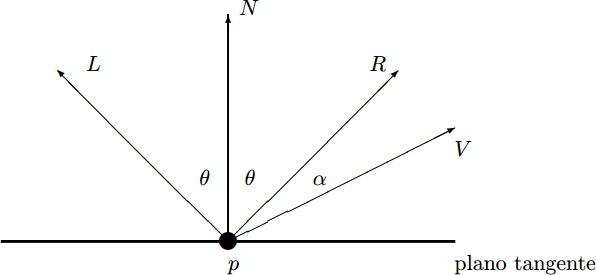
\includegraphics[width=11cm]{figures/phongVecs}
\caption[Vectores intervinientes en el cómputo de la BRDF de Phong]{Vectores intervinientes en el cómputo de la BRDF de Phong. La radiancia ingresa desde $-L$ hacia $p$. El observador se encuentra en $V$.}
\label{fg:phongVecs}
\end{figure}

El término ambiente en la ecuación, representa una aproximación a la radiancia dispersa por toda la escena, y está definido por una constante.

El término difuso de la BRDF del material no se modifica con respecto a la posición del observador.
El mismo resulta del cómputo del producto escalar entre la normal a la superficie y la posición de la fuente de luz.
En un extremo, el término difuso se anula cuando la luz incide perpendicularmente a la superficie.
El otro extremo se da cuando la normal coincide con la fuente de luz, en cuyo caso el término difuso toma su valor máximo.

La única modificación percibible por un observador al moverse, sobre la apariencia de una superficie modelada por la BRDF de Phong, está dada por el término especular.
Intuitivamente, a medida que el observador en $V$ se acerca a la dirección del rayo reflejado $R$, ocurre que $R$ se acerca a $V$. En el límite, $R = V$
y por lo tanto $R \cdot V$ asume un valor máximo.
A medida que el observador en $V$ se aleja de $R$, el producto escalar tiende a cero, y la reflectancia se percibe en menor medida.

Si bien el modelo responde a un diseño mayormente fenomenológico, el mismo resulta intuitivo y flexible.
Además, obtiene buenos resultados en superficies opacas de marcada especularidad, como metales y plásticos, entre otros.

\begin{figure}
\center
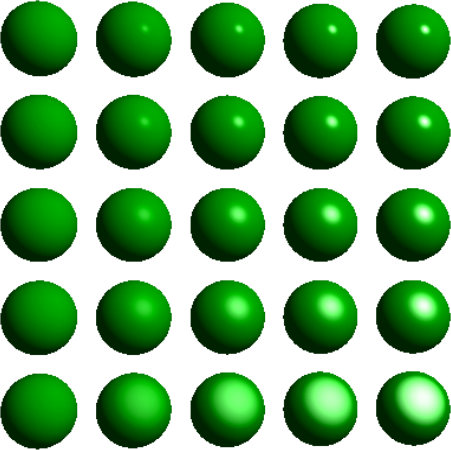
\includegraphics[width=9cm]{figures/phongparametros}
\caption[Diferentes apariencias en el modelo de Phong]{Diferentes apariencias obtenidas en una esfera, modificando parámetros en el modelo de Phong, para un observador y una fuente de luz fijos. De izquierda a derecha $k_{s}$ varía de $0$ a $1$. De arriba hacia abajo, $\alpha$ varía de $50$ a $1$.}
\label{fg:phongparametros}
\end{figure}

%\subsection{Radiosidad}

%\subsection{Ray Tracing}
%\subsection{Ray Marching}
%\subsection{Volume Rendering}
%\subsection{Photon Mapping}

\section{Materiales específicos}
Debido a la necesidad creciente en el modelado y renderizado realista de materiales, el diseño de BRDFs y métodos derivados de las ecuaciones del renderizado, y del renderizado de volúmenes, evolucionaron hacia representaciones más complejas, permitiendo representar una mayor cantidad de apariencias y materiales.
Además, y debido a las características particulares de determinados materiales, los métodos mencionados resultaron inadecuados de ser aplicados de manera directa.
Esto provocó que se desarrollaran técnicas específicas para materiales determinados.

En otras palabras, si bien las ecuaciones presentadas proveen un marco teórico general para los fenómenos resultantes de la interacción entre la energía radiante y los materiales en una escena, los detalles de implementación computacional (representación como superficie o volumen, escala de representación, consideraciones de almacenamiento, etc.) muchas veces dificultan su utilización directa, debiendo diseñarse soluciones particulares que atiendan a los requerimientos específicos de cada material.
Por ejemplo, la BRDF no siempre constituye la solución adecuada para modelar una superficie, escogiéndose en algunos casos otras representaciones, como una BSSRDF o una BTF.

Debido a esto, han surgido técnicas que han considerado distintos aspectos intentando obtener realismo en el renderizado.
Algunas optaron por sintetizar modelos de primeros principios. 
Entre ellas se encuentran la modelización del proceso de fabricación del material (por ejemplo en telas), o modelizar el comportamiento químico de determinados componentes que forman el material (piel).
Otras metodologías utilizaron un enfoque fenomenológico para la obtención de un modelo.
Entre estas técnicas encontramos el diseño de las microgeometrías presentes en superficies de materiales (cerámicos), y el uso de dispositivos de captura de determinadas propiedades del material (pinturas de autos). 


Esta sección presenta distintos ejemplos de diseño de materiales en computación gráfica con diversas metodologías.
Se desprende que el modelado y renderizado de materiales constituye aún un tema abierto, del cual sólo algunos ejemplos han sido desarrollados \cite{Dorsey2007}.
Existe aún un amplio abanico de materiales que requieren tratamiento.
Dependiendo del nivel de realismo deseado, se pueden aplicar diversas metodologías al diseño de los mismos.


\subsection{Piel}
Comenzaremos con un material extremadamente complejo y ubicuo en computación gráfica: la piel humana.
Debido a su extenso uso en aplicaciones gráficas, existen para este material un importante número de trabajos científicos, los cuales varían en complejidad, presentando diversos enfoques a la hora de realizar su modelado.
Un modelo poco preciso de la piel podría ser fácilmente detectado por humanos, con lo cual un diseño cuidado resulta crucial para alcanzar un realismo aceptable.


La composición de la piel está fuertemente estudiada en medicina.
Debido a esto, existen trabajos muy completos sobre su estructura y propiedades \cite{Walters2002}.
La piel está compuesta por diversas capas como la epidermis, la dermis y la hipodermis.
La más exterior es la epidermis, compuesta por células muertas.
A mayor profundidad aparece la dermis, la cual posee mayor espesor y vasos sanguíneos (lo cual afecta, entre otros, al color final de la piel).
La capa más interna resulta la hipodermis, conectando la piel con el cuerpo.
Todas estas capas presentan una estructura muy compleja.
Este material posee mucho dinamismo, pudiendo ser afectado por diversos factores, como el sol, lastimaduras, y variaciones en el torrente sanguíneo.
Su compleja estructura geométrica presenta poros y patrones característicos que varían para cada persona (por ejemplo las huellas dactilares).

La estructura de capas fue imitada en computación gráfica realizando abruptas simplificaciones.
De esta forma, se diseñó un modelo de reflectancia para su superficie (BRDF) junto con un modelo microgeométrico, y un modelo de dispersión debajo de la superficie (\acrshort{BSSRDF}) en una segunda capa.

Un ejemplo de síntesis de piel aparece en \cite{Marschner2000}, donde se utiliza una BRDF de Lafortune (definida como una generalización de la BRDF de Phong con varios lóbulos) para la reflectancia superficial, junto con texturas que se mapean sobre una geometría de la cara de una persona.
En otro trabajo se utilizó además información proveniente de moldes de polímeros presionados sobre la cara de personas \cite{Haro2001}, con el fin de capturar detalles finos de la geometría, utilizando además algoritmos de síntesis de imágenes para generar muestras más grandes que las medidas, ver Fig.~\ref{fg:piel}.

\begin{figure}
\center
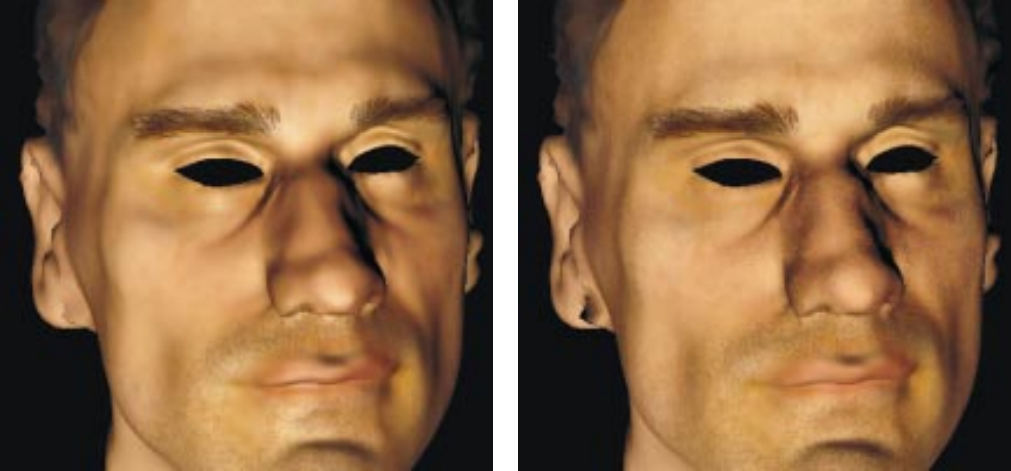
\includegraphics[width=9cm]{figures/piel}
\caption[Piel Humana renderizada]{Piel Humana renderizada con el método de \cite{Marschner2000}. La imagen de la derecha muestra la mejora obtenida al agregar detalles de geometría fina en el modelo (nariz, parte inferior del labio).}
\label{fg:piel}
\end{figure}

Un modelo basado en primeros principios puede verse en \cite{Krishnaswamy2004}.
En dicho trabajo se definen geometrías precisas para la dermis y epidermis, a partir de la cual se realizan simulaciones físicas estocásticas de rebote de la luz (simulaciones Monte Carlo), pudiéndose reconstruir una BRDF.
El modelo incluye muchos otros detalles de los procesos físicos intervinientes, como la intervención de la melanina y la bilirrubina, además de consideraciones de absorción, pigmentación, etc.

Existen trabajos que abordan otros aspectos del modelado de la apariencia de la piel.
El estudio de los patrones que produce el envejecimiento se estudia en \cite{Boissieux2000}.
Los mismos fueron medidos en muestras reales de una empresa cosmética.
La información geométrica fina puede obtenerse además a partir de imágenes \cite{Golovinskiy2006}.

Este ejemplo muestra con claridad que un mismo material puede presentar una amplia gama de modelos que simulan su apariencia, dependiendo de la aplicación específica y los detalles que se buscan representar.

\subsection{Materiales Porosos}

Determinados materiales porosos presentan micro-poros en la geometría de sus superficies.
Estos poros afectan de manera directa la noción de superficie contínua, asumida al modelar un material como una superficie y representar su comportamiento con la energía radiante por medio de una BRDF.

Estos poros microscópicos son aún más pequeños que los poros presentes en la piel humana.
Si bien su tamaño excede la longitud de onda de la luz, los mismos no son visibles al ojo humano.

Entre los pocos trabajos sobre estos materiales, se encuentra el de Merillou \cite{Merillou2000}.
En dicho trabajo se modifica la definición estándar de BRDF incluyendo términos matemáticos que representan la estructura y el comportamiento de materiales porosos.
Esto se logra a través de la modificación de los coeficientes especular ($k_{s}$) y difuso ($k_{d}$) de la BRDF, transformándolos en una {\em función} dependiente del ángulo de entrada y la posición del observador.

La idea intuitiva detrás de estas modificaciones constituye la profundización del modelo de dichos coeficientes, incluyendo el efecto de los poros sobre los mismos.
Por ejemplo, un rayo de luz que se comporta de forma especular, podría ser desviado por un poro y resultar {\em transformado} en energía difusa.
Esto se traduce en la dirección del rayo de rebote, ya que la presencia del poro provoca que el rayo que sería especular obtenga una dirección de salida posiblemente arbitraria.
Matemáticamente, el coeficiente difuso toma una parte del coeficiente especular.

Para obtener una distribución estadística de las geometrías de los poros presentes en una superficie, se deben modelizar los mismos.
El modelado de los poros se lleva a cabo por medio de simulaciones estocásticas Monte Carlo sobre posibles geometrías microscópicas de poros bajo ciertas asunciones.
Dos ejemplos diferentes de poros pueden observarse en la Fig.~\ref{fg:poro}.
Se simula el rebote de rayos de luz sobre la geometría sintetizada, computándose las distribuciones de reflectancia para poros con distintas formas, utilizando un máximo en el número de rebotes.
También resulta adecuado incorportar un factor de absorción en cada rebote, disminuyendo la radiancia del rayo siendo computado.
El proceso se repite para distintas simulaciones estocásticas de la geometría de los poros.


En la Fig.~\ref{fg:ceramico} podemos observar una imagen de una maceta renderizada con una BRDF tradicional, y a la derecha, la misma imagen utilizando la BRDF modificada por este método.

\begin{figure}
\center
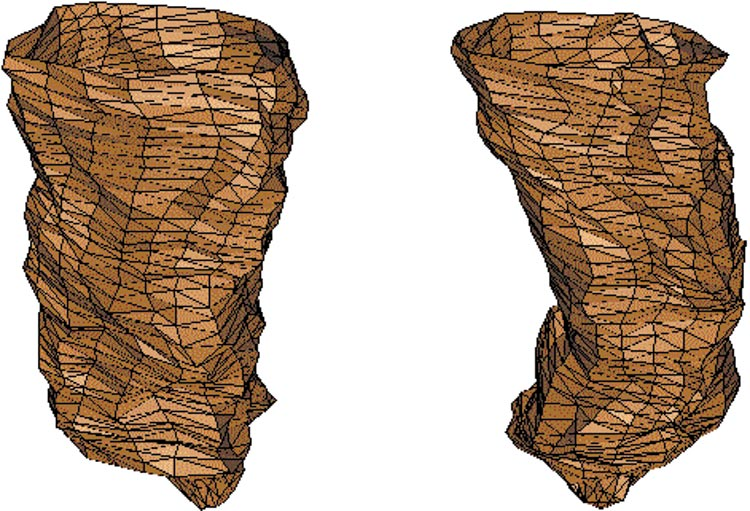
\includegraphics[width=8cm]{figures/poro}
\caption[Poros sinterizados]{Ejemplo de poros sintetizados utilizando el método desarrollado en \cite{Merillou2000}.}
\label{fg:poro}
\end{figure}

\begin{figure}
\center
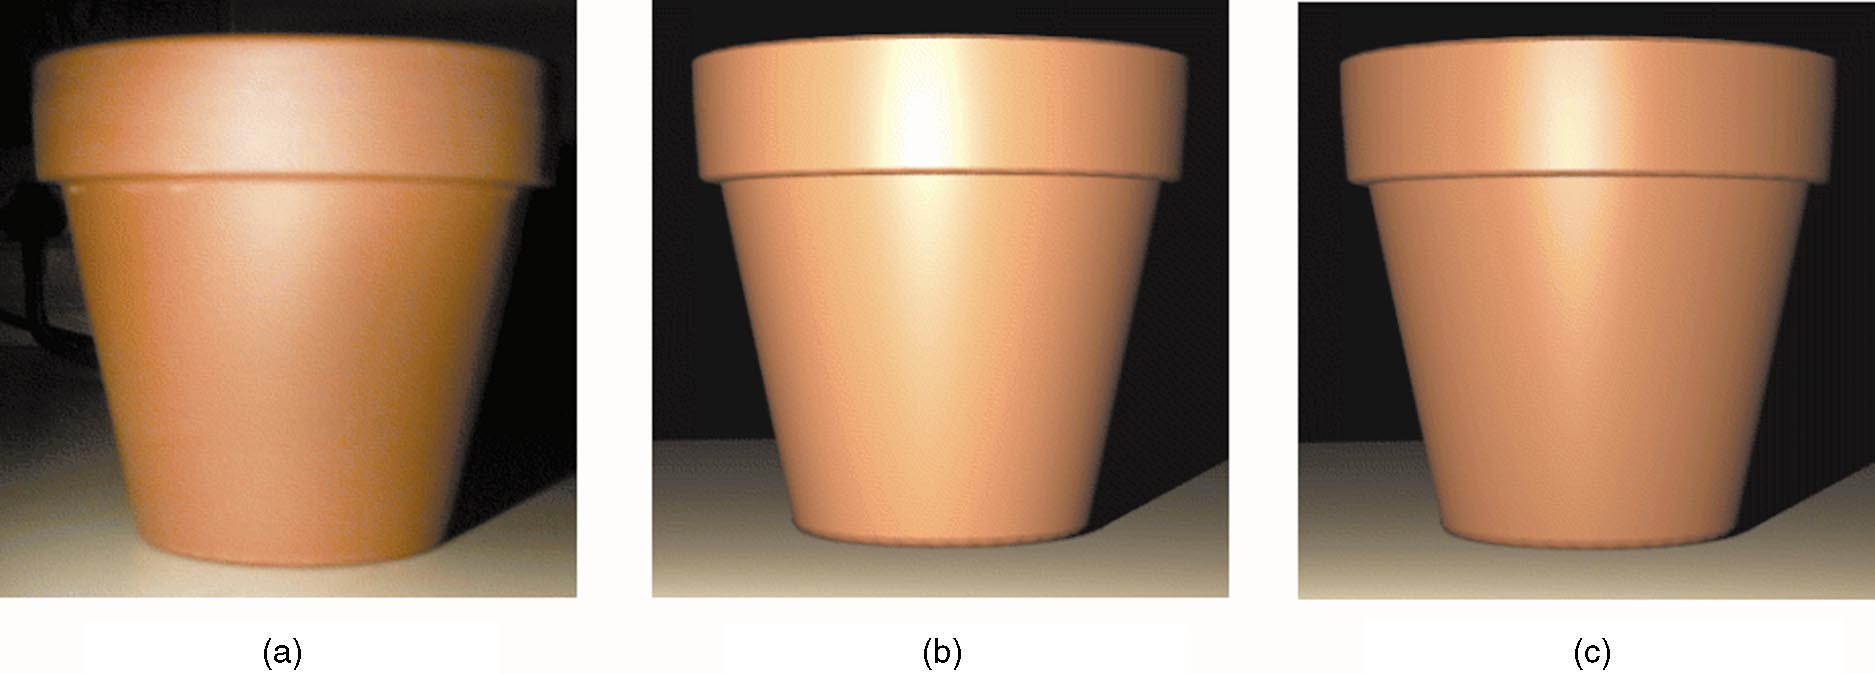
\includegraphics[width=11cm]{figures/ceramico}
\caption[Cerámicos renderizados]{Cerámicos renderizados. Izquierda: maceta real. Centro: utilizando una BRDF tradicional. Derecha: utilizando el método propuesto en \cite{Merillou2000}.}
\label{fg:ceramico}
\end{figure}

La tesis presente se ubica sobre este tipo de materiales, dado que el pan constituye un material poroso que involucra cocción previa.
A diferencia de los cerámicos, los poros son visibles por el ojo humano.

\subsection{Pelo}
Al igual que con los cerámicos y la piel, el modelado del pelo debe tener en cuenta su estructura interna.
Cada pelo individual consiste de tres partes principales: una médula central, el córtex y una cutícula exterior.
Su color está dado por gránulos de melanina en el córtex.
Cuando no están presentes estos gránulos se observa un color blanco.


Existen dos tipos principales de pelo : el {\em vello}, presente en prácticamente toda la superficie del cuerpo, con $1$ {\em mm} de alto; y el {pelo terminal}, presente únicamente en el cuero cabelludo.
Este último fue el que recibió mayor atención en computación gráfica.
El pelo terminal tiene aproximadamente entre $50$ y $90$ micrones de diámetro.
Existen entre $175$ y $300$ pelos terminales por {\em $cm^{2}$}.
El pelo de animales difiere del humano en color, tamaño, y densidad.

Cada pelo individual puede considerarse una superficie con dispersión lumínica propia.
Por otro lado, la apariencia típica del pelo está dada por el conjunto de muchos pelos individuales.
Sin embargo, utilizar soluciones volumétricas típicas, como modelar el pelo como se modela una nube o el humo no resulta adecuado, ya que la geometría del pelo afecta la reflectancia de la luz incidente.

Para solucionar estos inconvenientes se creó una estructura denominada {\em texel}, que no debe confundirse con un elemento de una textura.
Un texel se define como una {\em estructura de datos} volumétrica que asocia tres componentes: una densidad de área proyectada $\rho$, un marco de referencia $\bold{B}$ y un modelo bidireccional de reflexión de la luz $\psi$, a cada posición $3D$ del espacio.
La densidad de área proyectada $\rho$ se define como la fracción del área proyectada del {\em vóxel} (cada entrada en una matriz tridimensional) en una dirección particular cubierta por geometría del pelo proyectada en la misma dirección.
En $\bold{B}$, la orientación queda especificada por los vectores normal, binormal, y tangente.
Para determinar los vectores, se asume un cilindro general que crece desde la piel del cuero cabelludo.
$\psi$ se define como una variación del modelo de Phong, devolviendo la luz reflejada en el punto.
Los componentes difuso y especular del modelo son,

\begin{align*}
\psi_{d} &= K_{d} sin \theta_{i}\\
\psi_{s} &= K_{s} (cos \theta_{i} cos \theta_{r} + sin \theta_{i} sin \theta_{r})^{p},
\end{align*}

donde $\theta_{i}$ nota el ángulo entre la luz y la tangente al pelo, y $\theta_{r}$ el ángulo entre la tangente al pelo y el observador.

Luego, para calcular el color final de un pixel en pantalla, desde el punto de vista del observador, se recorren en línea recta, desde $t_{near}$ a $t_{far}$ según corresponda a ese pixel, los texels necesarios,

$$L = \sum_{t=t_{near}}^{t=t_{far}} {e^{-\tau \sum_{u=t_{near}}^{u=t} \rho(u)} \rho(t) \sum_{i} L_{i}(t) \bold{\psi}(t)},$$

donde la suma sobre $i$ refiere a las fuentes de luz, y $\tau$ representa un coeficiente que convierte las distribuciones de área proyectada en un coeficiente de atenuación.

Este método sirve para simular pelo corto, pero visto a cierta distancia, ver Fig.~\ref{fg:osopelo}.
La percepción de pelo se pierde cuando la cámara se acerca demasiado al objeto.

\begin{figure}
\center
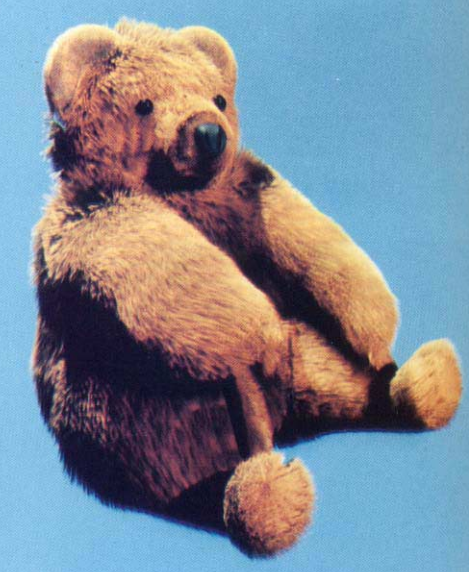
\includegraphics[width=6cm]{figures/osopelo}
\caption[Renderizado de pelo en un oso de peluche]{Ejemplo de renderizado de pelo en un oso de peluche con el método propuesto en \cite{Kajiya1989}.}
\label{fg:osopelo}
\end{figure}

%The projected area density is the fraction of the projected area of the voxel in a particular direction that is covered by hair geoemetry projected in the same direction

Es posible diseñar funciones $\bold{\psi}$ más realistas, teniendo en cuenta factores como la transmitancia y el impacto de las fibras individuales entre sí (iluminación indirecta).
Puede verse un estudio más completo de la literatura sobre renderizado de pelo en \cite{Ward2007}.

\subsection{Telas}
Las telas son un material similar al pelo en cuanto a su composición, ya que están formadas por un conjunto de fibras.
Las fibras de telas presentan diferentes {\em tinturas}.
Resulta importante considerar las tinturas que componen una fibra para entender la apariencia de una tela vista desde distintos ángulos.
Por ejemplo, determinadas fibras de telas presentan más de una tintura, como muestra la Fig.~\ref{fg:fibra}.
En este caso, los rayos de luz provenientes de distintas posiciones atraviesan distintas longitudes sobre las tinturas, produciendo iridiscencia, es decir, modificación del color visible dependiendo del ángulo de visión.

\begin{figure}
\center

\includegraphics[width=4cm]{figures/fibra}
\caption[Ejemplo de fibra de tela con más de una tintura]{Ejemplo de fibra de tela con más de una tintura. Se puede observar una tintura roja en el centro, y una tintura azul que la envuelve.}
\label{fg:fibra}
\end{figure}

La apariencia de cada tipo de tela difiere dependiendo del material utilizado (seda, lana, hilos, etc.) como del proceso de tejido en sí.
En \cite{Xu2001} se observa que determinados hilos están formados por un conjunto de fibras compactadas y con estructura helicoidal.
Esta observación se aplica para definir un texel específico como en el caso del pelo, el cual luego permite determinar la cantidad de luz que será emitida en una dirección para una dirección entrante, ver Fig. \ref{fg:tela}.
Para esto se tienen en cuenta efectos como sombras, oclusión y dispersión múltiple entre los distintos hilos que componen una tela.
Debe contarse además con una estructura coherente que conecte a los hilos, formando una tela realista.
Para esto se utilizan curvas $3D$ construídas a partir de los puntos de control definidos en la división de la superficie.


\begin{figure}
\center
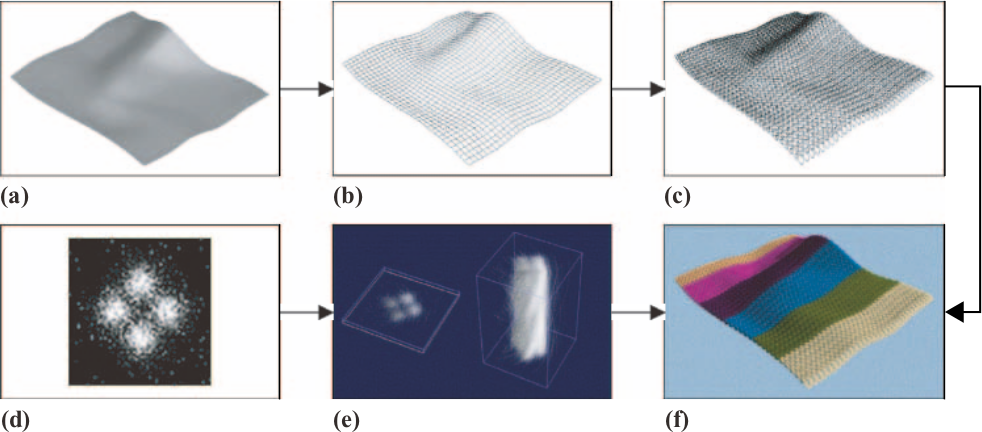
\includegraphics[width=13cm]{figures/tela}
\caption[Pasos para la definición de un modelo de una tela]{Pasos para la definición de un modelo de una tela, donde se toman en cuenta fibras individuales. Además de la utilización de una superficie (a), la misma se subdivide (b) para alojar distintas estructuras de hilo (c), los cuales se modelan individualmente ((d) y (e)).}
\label{fg:tela}
\end{figure}

\subsection{Pinturas de autos}
Determinadas marcas de automotores han expuesto la necesidad de una correcta visualización de las pinturas aplicadas sobre la superficie exterior de los mismos.
Los modelos desarrollados se han utlizado para presentar al público nuevos productos de estas fábricas, permitiendo a los posibles compradores configurar los colores y características deseadas en las pinturas.
Debido a esto, un modelo adecuado del material resulta imprescindible para permitir una reproducción lo más fiel posible al mismo, en un automóvil real.

Se han desarrollado principalmente dos categorías de métodos para obtener un material con la apariencia de pintura de automóviles: aquellos basados en primeros principios \cite{Ershov2001}, y los basados en capturas de características de pinturas reales.

En el primero se realiza un modelo por capas, donde cada capa contiene partículas de pigmentos como en las pinturas reales.
El modelo de dos capas presentado asume una capa con partículas que reflejan la luz especularmente, y la otra con una pintura opaca.
Tomando en consideración parámetros como la densidad, la distribución de las orientaciones de las partículas, la transmitancia y la reflectancia, derivan una compleja BRDF parametrizada y analítica que permite definir distintos tipos de pinturas, ver Fig.~\ref{fg:pinturaauto}.

Modelos basados en capturas reales utilizan distintas tomas de la radiancia saliente de la pintura de autos, combinándolas.
En \cite{Dumont2001} además se utilizan texturas que representan la microgeometría de las pinturas También se utilizó ruido para producir efectos como el denominado {\em brillo} (sparkle).
En otro trabajo \cite{Gunther2005}, se utilizaron los datos de las medidas para producir un modelo analítico estadístico del brillo.
Como puede observarse, diversas metodologías pueden producir el mismo material o el mismo efecto.
La elección final se toma en base a la complejidad de la captura, costos computacionales, objetivos, y realismo esperado, entre otros factores.

\begin{figure}
\center
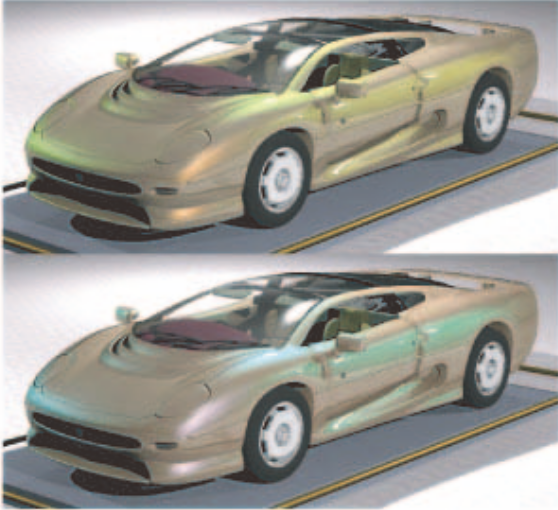
\includegraphics[width=8cm]{figures/pinturaauto}
\caption[Pinturas de autos diseñadas utilizando primeros principios]{Pinturas de autos diseñadas utilizando primeros principios en \cite{Ershov2001}. La variación de un parámetro permite obtener diferentes apariencias (en este caso, el espesor de las capas de interferencia).}
\label{fg:pinturaauto}
\end{figure}


\section{Conclusiones}
En este capítulo presentamos un resumen del estado del arte en modelado y renderizado de materiales en computación gráfica.
Del capítulo se desprende que la obtención de un modelo realista de un material dado, responde a una correcta modelización tanto su geometría como de su interacción con la luz, de la manera más realista posible.
Además, deben tenerse en cuenta los costos computacionales, la escala de la representación buscada, y el método utilizado para el renderizado del mismo (utilizar la ecuación del renderizado, modelando el material como una superficie, o diseñar el mismo como un volumen).

El pan ha sido un material elusivo en computación gráfica.
Se cuenta con un único trabajo en el tópico \cite{Tong2005}.
El enfoque utilizado resulta en un método de fuerza bruta, es decir, capturas de reflectancia e imágenes de la miga de pan desde un punto de vista puramente fenomenológico.
Además, no se realizan consideraciones sobre la geometría del mismo.
Estas y otras limitaciones severas del método fueron superadas en la presente tesis.

En los capítulos que siguen, mostraremos como el diseño de la geometría y la interacción lumínica, fueron claves para lograr un renderizado realista de la miga y corteza de diferentes tipos de panes.

 \cleardoublepage
\chapter[Modelado de la Geometría de Miga de Pan]{Modelado Procedimental de Geometrías de Miga de Pan y Otros Materiales Porosos}

\section{Introducción y Motivación} % (Películas de Animación)
Como fue previamente explicado, determinados materiales recibieron menor atención en la literatura científica, debido entre otros factores, a la dificultad en el modelado, a los altos costos computacionales, y/o a la necesidad de utilización del material en aplicaciones prácticas.
Con el paso de los a\~nos, la industria del cine y de los video juegos utilizó procedimientos artísticos que intentan subsanar estas deficiencias.
De esta forma, se busc\'o la mayor similitud posible entre el material sintetizado y el real, sin importar si el proceso es una simulación física o el resultado de un procedimiento artístico.
Entre los innumerables ejemplos que se pueden citar, uno particularmente relacionado al trabajo de esta tesis lo constituye la película Ratatouille \cite{Cho2007}.
La misma se desarrolla en un ambiente de cocina, y por lo tanto existen alimentos y materiales naturales que deben ser modelados para ser renderizados.
Debido a la inexistencia de modelos estándar de determinados materiales en la literatura de computación gráfica (comestibles), los artistas y programadores encargados de llevar a cabo la producción visual de la película debieron crear técnicas ad-hoc para lograr un renderizado realista de los diferentes materiales.
Sin embargo, el éxito visual obtenido no se vio acompañado de una liberación del código que producía dichas imágenes, por lo cual la técnica permaneció para uso privado de la compañía productora, resultando en una difícil reproducción de dichos materiales por parte de terceros.

En nuestro trabajo intentamos subsanar estas deficiencias.
Por un lado, la falta de modelos ad-hoc documentados y por lo tanto reproducibles, y por otro, la utilización de modelos físicos basados en los procesos reales de formación de los materiales, los cuales sin dudas provocarán que el resultado sintético posea una mayor similitud visual y estructural a los materiales que se pretenden representar.

\section{Un Framework para la Síntesis de Texturas de Materiales}
En primer lugar presentaremos un sencillo procedimiento, en dos dimensiones, que permite obtener texturas de distintos materiales.
Dichos materiales usualmente se presentan en publicaciones separadas en la literatura, dado que los procedimientos que producen las mismas son fuertemente diferentes.
El procedimiento presentado ser\'a luego derivado para obtener texturas de pan y otros materiales porosos.

%Una vez establecidas las texturas en computación gráfica como un método simple y eficiente de representar materiales, se idearon técnicas automáticas para generarlas.
%De esta forma, no se depende exclusivamente de imágenes para obtener las mismas.

\subsection{Sistemas de Partículas y Autómatas Celulares}
En un sistema de part\'iculas \cite{Reeves1983} t\'ipico las part\'iculas nacen, se desarrollan y mueren, respetando reglas que les son impuestas por el sistema. Estos sistemas intentan modelar la din\'amica del fen\'omeno a trav\'es del tiempo, siendo uno de sus principales intereses mostrar una animaci\'on del mismo \cite{Gao2010, Bagar2010, Lentine2010}.

Se propone utilizar estos sistemas como generadores procedimentales de texturas. Un enfoque similar puede observarse en \cite{Kranidotis98}, aunque el mismo no fue desarrollado en profundidad.
Aquí se sigue una linea de investigaci\'on similar, presentando un sistema de part\'iculas que est\'a caracterizado por el crecimiento de las mismas en cada iteraci\'on, las cuales ocupan texels asign\'andoles colores, pudi\'endose detener al mismo en la iteraci\'on que se crea conveniente, obteni\'endose una textura.
Las im\'agenes resultantes presentan aleatoriedad, lo cual es deseable en materiales naturales.
A trav\'es de la direcci\'on de crecimiento de las part\'iculas se producen distintos patrones visuales.

Es posible representar materiales cl\'asicos como madera, granito y m\'armol, pero tambi\'en otros como mosaicos, pinturas, vegetaci\'on, entre muchos otros.
En un trabajo anterior \cite{Baravalle2010} se abord\'o la generaci\'on procedimental de texturas.
La diferencia radica en el mecanismo de generaci\'on, dado que con esta nueva propuesta es un {\em proceso temporal} el que produce los resultados, con lo cual puede representarse todo el proceso de formaci\'on de un material.
Adem\'as, cada corrida del algoritmo produce una textura distinta utilizando los mismos par\'ametros, debido a la naturaleza aleatoria de la generaci\'on (aunque el uso de seeding permitir\'ia repetir texturas en el caso de requerirse, por ejemplo para generar baldosas id\'enticas).

Se utiliza como plataforma de implementaci\'on a WebGL\footnote{\em http://www.khronos.org/webgl/}, recientemente propuesta por el Khronos Group (Open Standars for Media Authoring and Acceleration), dado que la misma otorga portabilidad al modelo. 
Programadores pueden incluirlo como biblioteca en aplicaciones gr\'aficas.
Dise\~nadores pueden utilizar la implementaci\'on para producir materiales, dada la intuitividad de los par\'ametros del mismo.

\subsubsection{Desarrollo}
Inicialmente el sistema consta de un conjunto de part\'iculas $P$
\begin{equation}
P = \{p_{1}, ... , p_{n}\}, n  \in \mathbb{N},
\end{equation}
uno o varios colores {\em RGB}, los cuales pueden tomar las part\'iculas.
\begin{equation}
cols = \{col_{1}, ... , col_{m} \}, m \in \mathbb{N},
\end{equation}
un conjunto de direcciones de crecimiento $D$,
\begin{equation}
D = \{d_{1}, ... , d_{k} \}, k \in \mathbb{N},
\end{equation}
y una grilla $B_{N\times N}, N \in \mathbb{N} $ de texels con colores RGB asociados (inicialmente $(R,G,B)=(0,0,0)$).

Cada elemento del conjunto $P$ posee las siguientes propiedades:
\begin{equation}
p_{i} = \{T_{i}, C_{i}, d_{i}, color_{i}\}, 1 \le i \le n,
\end{equation}
donde:

$T_{i} = \{t_{1}, ... , t_{n_{i}}\}$: conjunto de texels {\em ocupados} por la part\'icula en $B$,

$C_{i} = \{c_{1}, ... , c_{m_{i}}\}$: conjunto de texels {\em contorno} de la part\'icula en $B$,

$d_{i} \in D$: direcci\'on de crecimiento,

$color_{i}$: color {\em RGB} de la part\'icula, con ecuaci\'on \cite{Reeves1983}
\begin{equation}
color_{i} = col_{h} + rand * varcolor,
\label{eqColor}
\end{equation}

\noindent
y donde rand es un n\'umero pseudo-aleatorio uniformemente distribuido entre $-1$ y $1$, $varcolor$ un par\'ametro y $col_{h} \in cols$.
Cada $t \in T_{i}$ tiene asociado un color que var\'ia con respecto a $color_{i}$, de similar manera a la ecuaci\'on (\ref{eqColor}).

El {\em contorno} de una part\'icula determina los texels que la misma puede incorporar. 
En cada iteraci\'on, se elige aleatoriamente un texel en $C_{i}$, se lo quita del mismo y se lo incorpora a $T_{i}$.
Luego se actualiza el contorno de acuerdo a $d_{i}$ y al nuevo texel incorporado.
Se repite el proceso $\forall p_{i} \in P$, respetando las siguientes restricciones:
\begin{eqnarray}
\forall p_{i}, p_{j} \in P, t \in T_{i} \Rightarrow t \notin T_{j}, \\
\forall p_{i} \in P, t \in T_{i} \Rightarrow t \notin C_{i}.
\end{eqnarray}

Es decir, si una part\'icula posee un texel en $T_{i}$, ninguna otra lo posee (las part\'iculas son disjuntas), y si una part\'icula posee un texel en $T_{i}$, \'este no est\'a en su contorno.

Las part\'iculas pueden {\em nacer} y {\em morir}, lo cual representa su inclusi\'on o eliminaci\'on de $P$.
Al morir, la part\'icula deja asociados los colores de su conjunto $T_{i}$ en $B$, pudiendo utilizarse posteriormente esta informaci\'on.

Podemos intentar aplicar estas técnicas al modelado procedimental de texturas. 

En la Fig.~\ref{resultados} se observan algunas im\'agenes sintetizadas.
En la primera fila, la primera y cuarta textura muestran patrones con direcci\'on vertical, direcci\'on elegida para hacer crecer a las part\'iculas.
La \'ultima figura de la segunda fila, muestra part\'iculas que crecen en 3 direcciones posibles: aleatorio ($50\%$), vertical ($25\%$) y horizontal ($25\%$), lo cual demuestra que se posee un control preciso sobre las formas resultantes en las texturas.
En la Figura \ref{sintesis} se observa un ejemplo de s\'intesis.
De izquierda a derecha, se observan texturas obtenidas en las iteraciones $10$, $150$, $250$, $500$ y $1000$.
En la Figura \ref{teteras} se observan texturas sintetizadas aplicadas a un objeto mediante texture mapping, mostrando una calidad aceptable para ser utilizadas en aplicaciones gr\'aficas.
La Figura \ref{muerte} muestra el efecto de muerte de part\'iculas.
Las mismas liberan el espacio en $T_{i}$ dejando asociado su color en $B$, permitiendo que las dem\'as puedan crecer en dichos texels.
De esta forma, puede utilizarse posteriormente la informaci\'on que la misma dej\'o asociada.
En este caso los colores de la part\'icula que libera el espacio y la ocupante fueron mezclados, obteni\'endose im\'agenes que parecen haber sido ``pintadas'' por capas.
%En la Figura \ref{software} se observa el modelo corriendo en un navegador web.


\begin{figure}[t!]
\centering
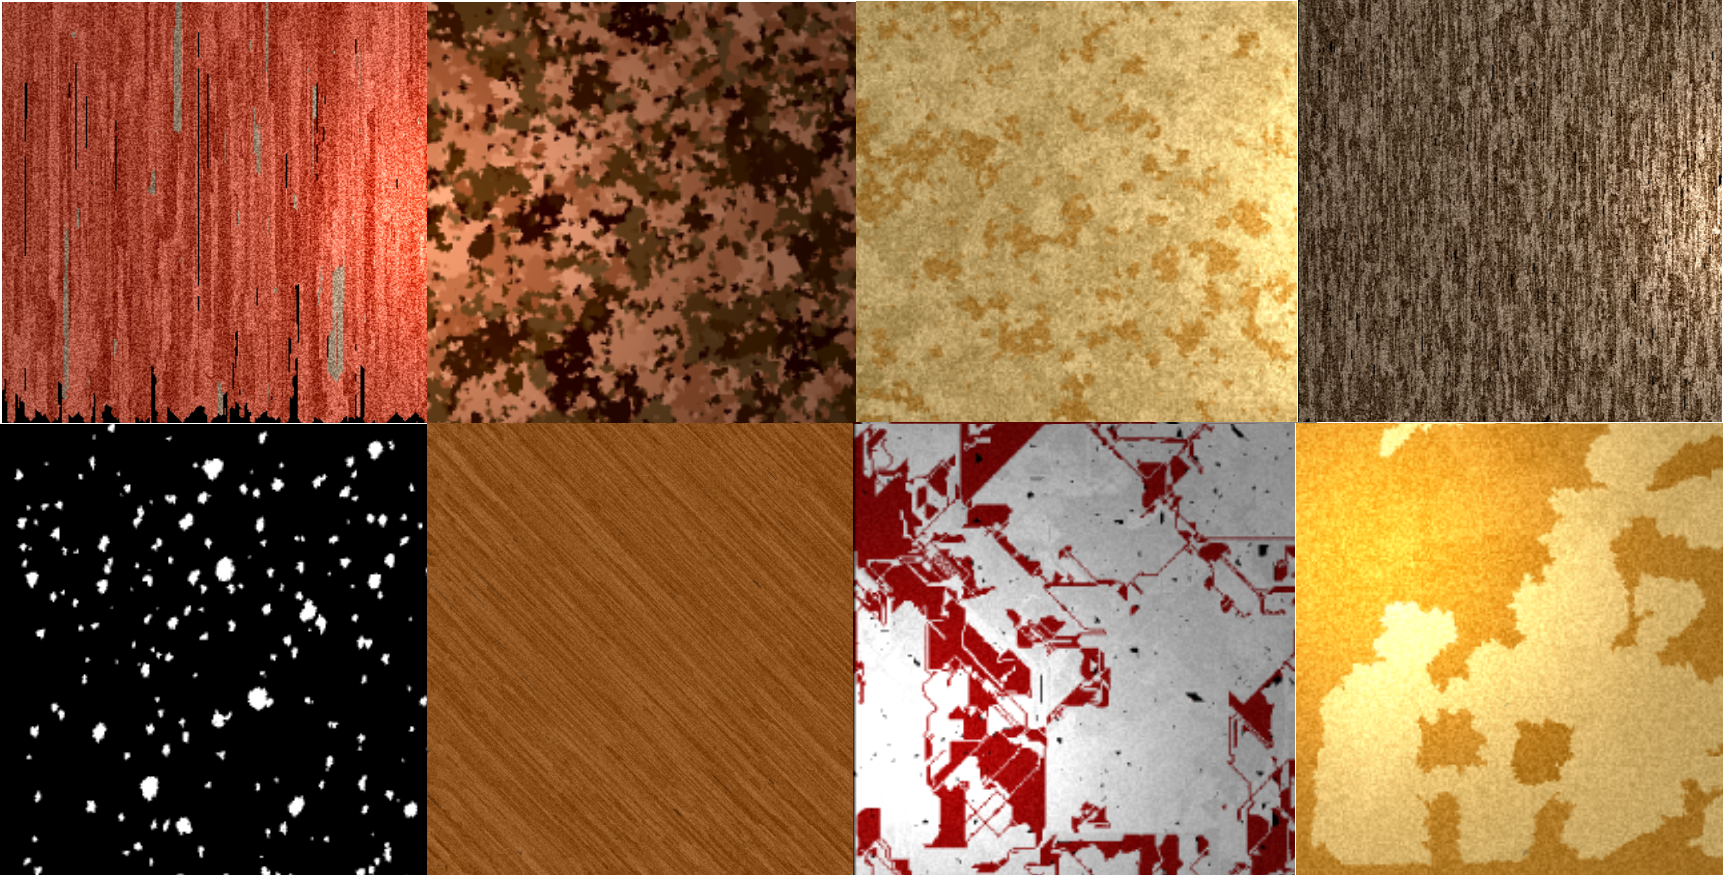
\includegraphics[scale=0.18]{resultados}
\caption{Distintas texturas sintetizadas utilizando sistemas de partículas.}
\label{resultados}
\end{figure}

Se muestra un ejemplo de s\'intesis de una textura en la Figura \ref{sintesis}. Deben seleccionarse los siguientes par\'ametros:

\begin{itemize}
\item Par\'ametro {\em cantidad de part\'iculas iniciales}, con valor $100$.
\item Par\'ametro {\em nuevas particulas por iteraci\'on}, con valor $1$.
\item Par\'ametros {\em color 1 y 2 (RGB)}. con colores de ejemplo, uno con la componente verde mayor y otro con mayor componente azul.
\item Par\'ametros {\em direcciones}: aleatorio: $50\%$, diagonal $50\%$.
\item Par\'ametro {\em variaci\'on de color}, con valor 0.1, en una escala [0,1] (ver $varcolor$ en la secci\'on anterior).
\item Par\'ametro {\em variaci\'on de color por part\'icula}, con valor 0.1, en una escala $[0,1]$, el cual determina la variaci\'on del color por texel dentro de la part\'icula.
\end{itemize}

\begin{figure}[t!]
\centering
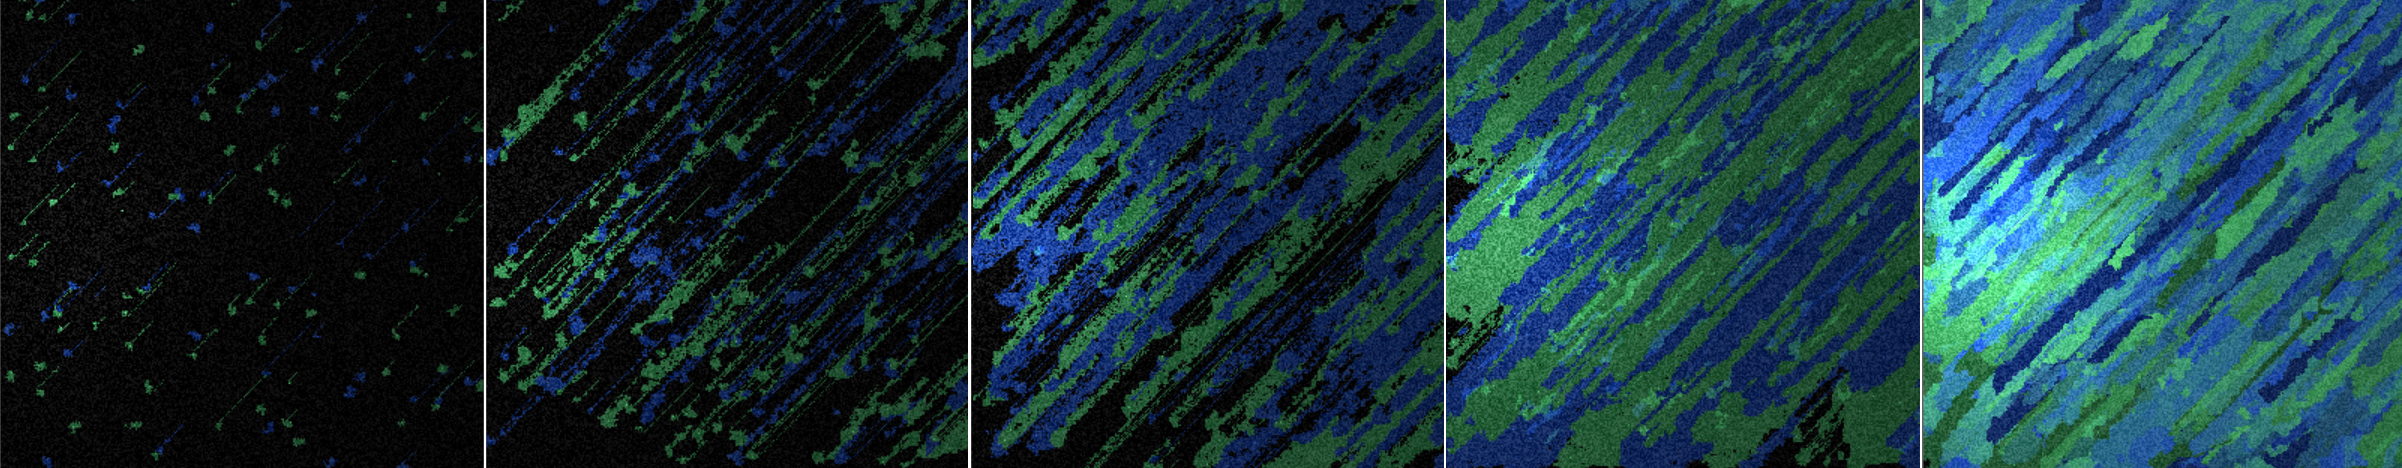
\includegraphics[scale=0.12]{sintesis}
\caption{Ejemplo de s\'intesis de una textura.}
\label{sintesis}
\end{figure}

\begin{figure}[t!]
\centering
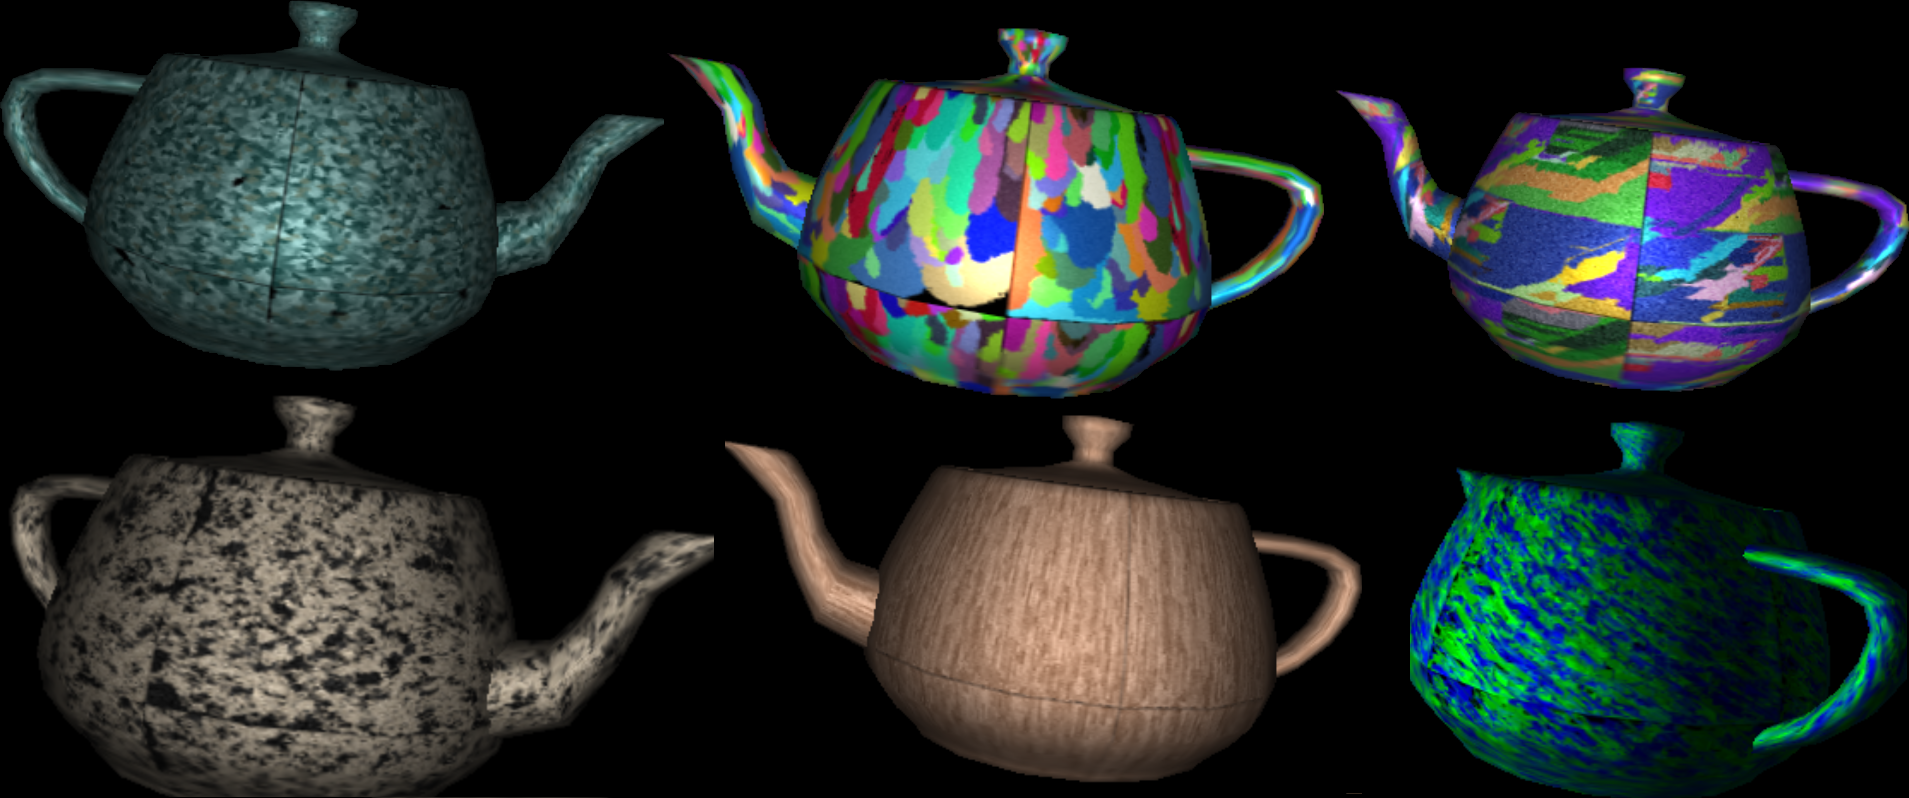
\includegraphics[scale=0.14]{teteras}
\caption{Texturas generadas mapeadas en una tetera.}
\label{teteras}
\end{figure}


\begin{figure}[t!]
\centering

\includegraphics[scale=0.2]{muerte}
\caption{Efecto producido utilizando el concepto de muerte de las partículas.}
\label{muerte}
\end{figure}

Los resultados obtenidos muestran una flexibilidad útil para producir distintos materiales.
La idea de utilizar sistemas de partículas para producir materiales será utilizada en la sección siguiente.
Más específicamente para producir geometrías de materiales porosos, particularmente la miga de pan.
Para esto, se generalizarán los resultados a tres dimensiones.

\section{Modelado Procedimental de la Geometría de la Miga de Pan}
En esta sección introducimos un modelo procedimental que permite realizar simulaciones de la geometr\'ia de la miga de pan, basado en el framework introducido en la secci\'on anterior.
Si bien el modelo introducido no está basado en primeros principios, el mismo es un paso previo que permite sentar las bases de un modelo inspirado físicamente.

\subsection{Introducción}
La inmensa variedad de materiales, y sus complejas interacciones con fuentes lumínicas, han sido un tópico central de investigación en las últimas décadas en Computación Gráfica.
El modelado de la naturaleza en física ha demostrado capturar de manera muy precisa fenómenos de transporte de la luz.
Las aproximaciones computacionales a estos modelos son una de las ramas más investigadas en el renderizado de materiales.
El modelado geométrico de materiales sigue una estrategia de investigación similar. Primero se construye un modelo físico del material, el cual luego es aproximado computacionalmente.
Debido a estas observaciones, el renderizado foto-realístico de materiales debe considerar tanto el modelado geométrico de los mismos como su interacción con la luz, para lograr una aproximación adecuada del material.

La elección del modelo geométrico depende de cada material, y de la escala de representación buscada.
Esta elección influencia fuertemente el algoritmo de renderizado. 
Existen dos tipos principales de modelado de materiales: superficies y volúmenes.
Para esto existen dos ecuaciones principales.
Por un lado, la ecuación del rendering \cite{Kajiya1986} captura la microgeometría de los materiales y su interacción con la luz en superficies.
Por otro, la ecuación del rendering de volúmenes \cite{Kajiya1984} modela fenómenos volúmetricos como la transmitancia, la extinción, etc., debido a propiedades del medio (o material).

Si el material a representar es homogéneo (metales, plásticos, y similares), la elección típica es utilizar una superficie para representar el mismo \cite{Neumann1999}.
Esta elección modela la superficie del material asumiendo distribuciones estadísticas en su microgeometría.
Para lograr capturar detalles mesoscópicos, por ejemplo en el caso de maderas o ladrillos \cite{Lefebvre2000}, una técnica usual es precomputar dichas características en texturas, las cuales luego son mapeadas en la superficie.
La utilización de superficies es usualmente menos costosa computacionalmente, pero por otro lado impone limitaciones al realismo que se puede alcanzar, sobre todo en aquellos detalles que son propios de la estructura a nivel mesoscópico y la interacción de la misma con la luz (por ejemplo luz que pasa a través de agujeros en una superficie).

Siguiendo este razonamiento, la miga del pan es un material extremadamente complejo de capturar, modelar y renderizar, debido a la geometría a distintos niveles (microscópico y mesoscópico) y su resultante interacción y fenómenos lumínicos.
De esta forma, la utilización de superficies no es adecuada bajo ningún punto de vista, ya que la textura del pan está dada en gran medida por los fenómenos previamente explicados.
Si bien es cierto que existen métodos en la literatura que utilizan superficies para representar características mesoscópicas de los materiales como funciones de texturas bidireccionales (bidirectional texture functions, BTF) \cite{Tong2002}, las mismas no manejan adecuadamente la interacción lumínica antes mencionada.
Existe un intento en la literatura por suprimir esta falta \cite{Tong2005}.
El método produce imágenes realistas, pero existen muchas dificultades prácticas en la captura, el cómputo y el renderizado.
Estas limitaciones provocan que la utilización de dicho método no sea práctica por el momento.
Además, el método resulta inflexible dado que para cada imagen del material es necesario repetir todo el proceso (dos imágenes distintas del material requieren dos capturas).
Tampoco es posible obtener cortes del mismo, dada la naturaleza de superficie del método.

Por otro lado, existen numerosas publicaciones que tratan el modelado de materiales mejor adaptados a una representación volumétrica (por ejemplo humo o nubes) \cite{Chentanez2011,Zhou2008}.
La utilización de volúmenes es costosa computacionalmente pero presenta varias ventajas. Una de ellas es que no depende de una malla de triángulos, como en el caso de las superficies, y por lo tanto no presenta las desventajas mencionadas para las mismas.

Finalmente, existe un compromiso al momento de modelar materiales complejos y elegir una representación adecuada.
Donde se requiere simplicidad y velocidad (posiblemente tiempo real), se utilizan superficies, en cambio, si el foto-realismo es el objetivo final, es más adecuado optar por una representación volumétrica.
En los últimos años esta elección se ve perturbada por la aparición de hardware paralelo de alta velocidad (placas gráficas o GPUs), ya que un diseño adecuado podría alcanzar imágenes foto-realistas utilizando volúmenes en tiempos interactivos.
Esto es lo que presentaremos a continuación.


En este capítulo proponemos una representación volumétrica para la geometría de la miga de pan, alcanzando incluso tasas de refresco de tiempo real.
Existe un intento similar en la literatura \cite{Perlin1989}, el cual utiliza funciones algebraicas que representan la geometría del material.
En nuestro caso, para ganar flexibilidad de diseño, utilizamos los sistemas de partículas previamente mencionados, en un cubo (tres dimensiones), en conjunto con sistemas dinámicos \cite{Strogatz2001} que provocan una evolución del sistema, produciendo patrones con formas geométricas naturales.
Este es un intento por simular el efecto de la levadura en la masa cruda del pan.
Estos procedimientos producen distribuciones de burbujas de distintos tamaños, resultando en un mecanismo controlable, que presenta propiedades estadísticas.
El sistema es capaz de generar imágenes foto-realistas de diversos tipos de pan, como se mostrará más adelante.

\section{Sistemas Dinámicos como Modelo de Miga de Pan}
El prop\'osito de este algoritmo es producir una geometr\'ia la cual se renderizar\'a posteriormente. Por lo tanto, en lugar de devolver el color de una posici\'on espec\'ifica, el algoritmo genera un campo escalar compuesto de $0$s y $1$s ($0$ si la posici\'on contiene aire, $1$ si la misma contiene masa).
Esta representaci\'on resulta adecuada para ser renderizada utilizando DVR.

El sistema consta de un conjunto de part\'iculas $P$,

\begin{equation}
  P = \{p_{1}, ... , p_{n}\}, n  \in \mathbb{N},
\end{equation}

\noindent una grilla $L_{N\times N \times N}, N \in \mathbb{N} $ (inicialmente $L_{xyz}=1$) de masa y aire como fue descripto previamente, y otra grilla $L^{2}_{N\times N \times N}$, (inicialmente $L^{2}_{xyz}=-1$) de posiciones donde cada celda almacena un único entero que indica qu\'e part\'icula es due\~na de la misma ($i$ si el elemento de la grilla pertenece al contorno o interior de la part\'icula $i$).

Cada elemento en $P$ posee las siguientes propiedades:

\begin{equation}
  p_{i} = \{O_{i}, C_{i}\}, 1 \le i \le n,
\end{equation}

\noindent donde:

\begin{itemize}
\item $O_{i} = \{o_{1}, ... , o_{n_{i}}\}$: (Ocupadas) vector (conjunto) de posiciones ocupadas por la part\'icula en $L$.

\item $C_{i} = \{c_{1}, ... , c_{m_{i}}\}$: (Contorno) vector (conjunto) de posiciones representando el {\em contorno} de la part\'icula en $L$.
\end{itemize}

El vector $O$ representa las posiciones que ser\'an afectadas por la part\'icula, y el contorno $C$ se utiliza para asegurar que las part\'iculas se eviten entre s\'i.

El algoritmo se describe, simplificadamente, en Algoritmo $1$. 

\begin{algorithm}[h!]
\caption{Algoritmo de modelado}
\begin{algorithmic}

\State{$t  = 0$}
\Comment{tiempo - iteración}
\State{$P  = []$}
\Comment{partículas}
\State{$L  = matriz(MxMxM).valores\_iniciales(1)$}
\Comment {Geometría - iniciada a 1 (masa)}
\State{$L^{2} = matriz(MxMxM).valores\_iniciales(-1)$}
\Comment{Dominio de cada partícula}

\For{$i \in [1,Cantidad\_Particulas]$}
    \Comment{Cada partícula toma una posición aleatoria en L}
    \State{$x \gets aleatorio, y \gets aleatorio()$}
    \State{$O[i] \gets [[x,y]]$}
    \State{$C[i] \gets []$}
    \For{$v \in vecindario(x,y)$}
        \State{$C[i].agregar(v)$}
    \EndFor
    \State{$P.agregar([O[i],C[i]])$}
\EndFor

\For {$t \in [0,tiempo\_max]$}
    \For {$i \in [1,Cantidad\_Particulas]$}
        \If {$vacio?~C[i]$}
            \State{morir()}
        \EndIf
        \For{$h \in C[i]$}
            \State{$C[i].eliminar(h)$}
            \Comment{la posición ya fue explorada}
            \State{// Si la posición o el contorno pertenece a otra partícula, elegir otra posición}
            \State{// borde\_libre chequea que el vecindario no este dominado por otra partícula}
            \If{$!(L^{2}[h] > 0 ~\&\&~ L^{2}[h] != i ~\&\&~ borde\_libre(separacion)$}
                \State{// Posición libre, ocupar}                
                \State{$L[h] \gets 0$} \Comment{masa -> aire}
                \State{$O[i].agregar(h)$}
                \State{$C[i].agregar(vecindario(h))$} 
                \State{$L^{2}.setear(vecindario(h),i)$} \Comment{Marcar posiciones en $L^{2}$ como $i$}
                \State{$L^{2}.setear(h,i)$}
                \Comment{turno de la particula $i+1$...}
            \EndIf
        \EndFor
    \EndFor
\EndFor
\end{algorithmic}
\end{algorithm}

Cuando $t = 0$, un conjunto de part\'iculas iniciales toman posiciones aleatorias en la grilla. Para cada partícula, la posici\'on elegida es la primera posici\'on ocupada en $O$, adem\'as, el vecindario de $O$ es agregado a $C$. Cada part\'icula evoluciona en un intento por extender sus posiciones ocupadas ($O$), marcando posiciones en $L$. Las posiciones se toman de $C$. Cuando una part\'icula ocupa una posici\'on, la misma se elimina de $C$ y se agrega a $O$. Luego el vecindario de esa posici\'on se agrega a $C$ (es decir las posiciones que rodean inmediatamente a la posici\'on tomada). Las grillas se actualizan de la siguiente manera: $L$ se setea a $0$ en la posici\'on y $L^{2}$ se setea con el valor $i$ en las posiciones que se agregan a $C$. Las part\'iculas s\'olo pueden crecer si el valor encontrado en $L^{2}$ no pertenece a otra part\'icula. El tama\~no del vecindario es un par\'ametro que define la distancia entre part\'iculas. Si el vector $C$ est\'a vac\'io, la part\'icula {\em muere} ya que no puede continuar creciendo.


El algoritmo puede ser terminado en cualquier $t$ deseado. El mismo puede finalizar su c\'omputo ante determinados eventos, por ejemplo, cuando todas las posiciones de $L^{2}$ fueron tomadas por part\'iculas, ya que no pueden realizarse progresos.

Variando el par\'ametro de distancia entre part\'iculas (separación) se obtienen distintas estructuras (ver Fig.~\ref{fg:sistdin1}). Las im\'agenes muestran ejemplos 2D (para mayor claridad) de crecimiento aleatorio de part\'iculas. La regi\'on blanca en las im\'agenes representa la masa restante luego del proceso.


\begin{figure*}[htb!]
  \centerline{
\includegraphics[width=13cm]{sistdin1}}
  \caption[Efecto del parámetro separación entre partículas.]{Efecto del parámetro separación entre partículas. Izquierda: separaci\'on = 1, centro: separaci\'on = 2, derecha: separaci\'on = 4.}
  \label{fg:sistdin1}
\end{figure*}

Finalmente, el algoritmo devuelve la grilla $L$, la cual ser\'a renderizada posteriormente. En la siguiente secci\'on se explica la utilizaci\'on de sistemas din\'amicos en la evoluci\'on guiada de part\'iculas.

\subsection{Sistemas Din\'amicos}

Las ecuaciones diferenciales tienen como prop\'osito tratar con la dificultad (o imposibilidad) de hallar soluciones anal\'iticas en procesos din\'amicos. En primer lugar, se define un modelo matem\'atico del problema, del cual luego se obtienen 
las ecuaciones diferenciales asociadas. Los mismos se resuelven por medio de aproximaciones num\'ericas en cada instante de tiempo.

Los costos computacionales de estas soluciones dependen de la complejidad del problema y el n\'umero de ecuaciones del sistema. En este trabajo proponemos utilizar una sub-\'area de ecuaciones diferenciales llamada ecuaciones diferenciales ordinarias (ODE). En esta representaci\'on, el tiempo es tratado como la \'unica variable independiente.


De manera general, las ODEs se representan utilizando el siguiente sistema de ecuaciones:
\begin{equation} \label{eq:simple}  
  \begin{aligned}
    \dot{x_{1}} = f_{1}(x_{1},\ldots,x_{n}),\\
    \ldots\\
    \dot{x_{n}} = f_{n}(x_{1},\ldots,x_{n}),
  \end{aligned}
\end{equation}

\noindent donde $\dot{x_{i}}$ representa la derivada de $x_{i}$ con respecto
a $t$. Las variables $x_{i}$ y las funciones $f_{i}$ se definen de manera diferente para cada problema. En este caso, cada variable representa una coordenada cartesiana en el espacio, $x_{1}$ es $x$, $x_{2}$ es $y$ y $x_{3}$ es $z$. El conjunto de $f_{i}$ ser\'a definido tratando de capturar la estructura interna del pan. La siguiente secci\'on muestra cómo estos sistemas pueden describir la evoluci\'on de los sistemas de part\'iculas.

\subsection{Evoluci\'on de sistemas de part\'iculas utilizando sistemas din\'amicos}

La percepci\'on humana puede detectar patrones en la estructura de la miga de pan. Distintas observaciones pueden realizarse sobre la distribuci\'on de las burbujas en la misma (ver Fig.~\ref{fg:panreal}). Primero, la forma de las burbujas cercanas a la corteza tiende a estirarse paralelamente a la misma. Esto es resultado de la acci\'on de las elevadas temperaturas durante la cocci\'on de la masa. Tambi\'en resulta evidente que la estructura completa es similar a un fluido con la forma de la corteza.


\begin{figure*}[htb!]
  \centerline{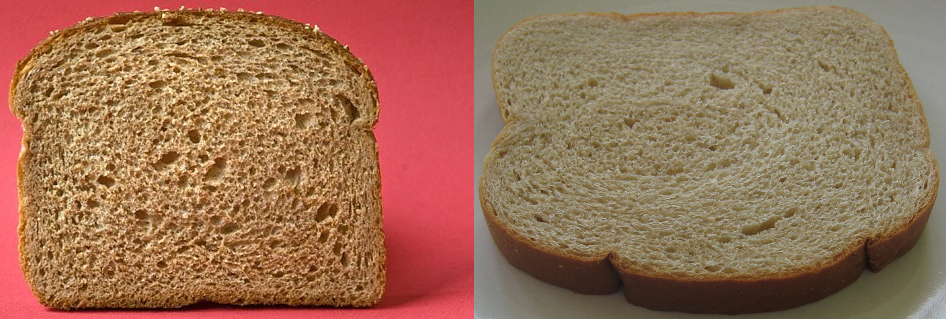
\includegraphics[width=13cm]{panreal}}
  \caption{Imágenes de cortes reales de pan}
  \label{fg:panreal}
\end{figure*}

Por otro lado, los sistemas din\'amicos previamente presentados producen formas naturales (ver Fig.~\ref{fg:sistdin2}). En las im\'agenes pueden observarse c\'irculos y espirales, entre otras formas. Las im\'agenes se obtuvieron dibujando trayectorias sobre un plano, siguiendo distintas ODEs. Tres ODEs describen las din\'amicas presentes en las im\'agenes. A modo de ejemplo, la imagen de la izquierda es el resultado del siguiente conjunto de ecuaciones:

\begin{equation} \label{eq:simple}  
  \begin{aligned}
    \dot{x} &= x^{2}-y^{2}+1,\\
    \dot{y} &= 2xy+1.
  \end{aligned}
\end{equation}


\begin{figure*}[htb!]
  \centerline{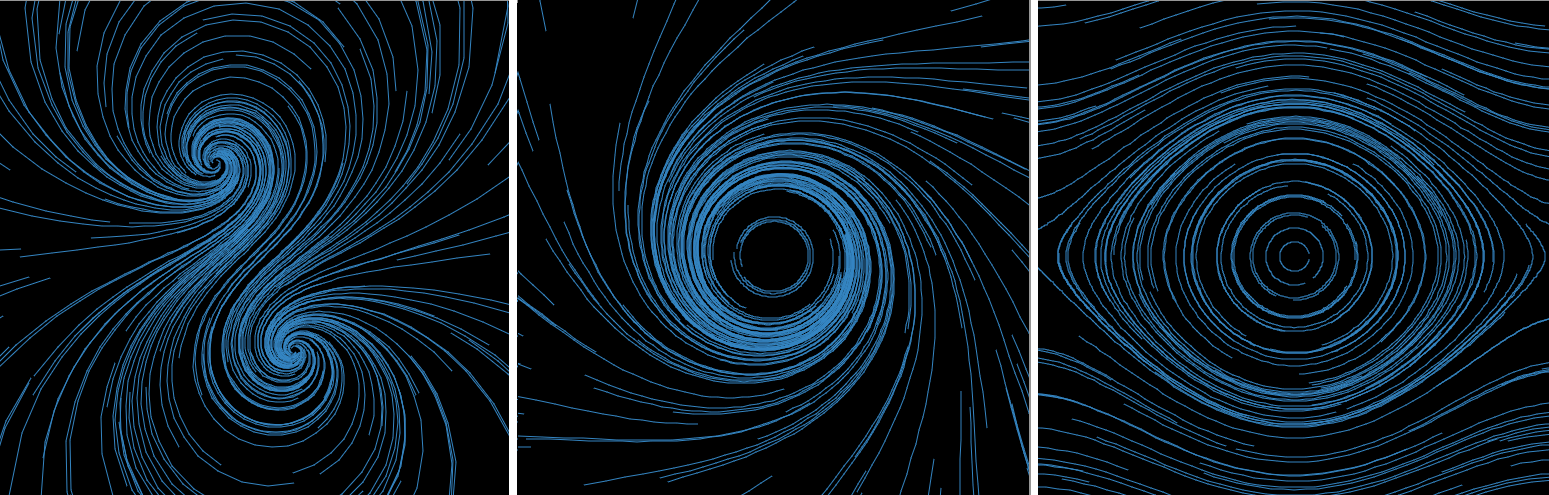
\includegraphics[width=13cm]{sistdin2}}
  \caption{Sistemas dinámicos en el plano.}
  \label{fg:sistdin2}
\end{figure*}

En los ejemplos se eligen posiciones aleatorias y luego el sistema se resuelve por medio de un {\em solver} Runge-Kutta de cuarto orden, el cual permite conocer la direcci\'on a tomar en cada punto por la trayectoria (en las im\'agenes se computaron trayectorias hacia adelante y hacia atrás en el tiempo para lograr una mejor visualizaci\'on). La imagen de la izquierda muestra un atractor y un repeledor claramente visibles. El centro de la espiral m\'as a la izquierda es un atractor (a medida que $t$ avanza, las trayectorias convergen hacia el punto), mientras que el otro centro es un repeledor. Los atractores pueden no ser puntuales, como muestran las restantes dos im\'agenes. La imagen de la derecha muestra atractores en forma de c\'irculos (las trayectorias ciclan por el c\'irculo).

Las part\'iculas producen distintos patrones al seguir las trayectorias definidas en el plano y el espacio. Esto se logra resolviendo num\'ericamente el sistema din\'amico en la posici\'on agregada a la part\'icula, seleccionando como siguiente posici\'on de crecimiento aquella posici\'on del contorno que mejor aproxima la soluci\'on del sistema din\'amico (para esto, sólo se agrega al contorno esa posición). El Algoritmo $2$ muestra cómo se modifica el algoritmo de modelado para incluir este comportamiento.

\begin{algorithm}[h!]
\caption{Modificación del algoritmo de modelado por medio de sistemas dinámicos}
\begin{algorithmic}
\State $L[h]\gets 0$ \Comment{masa $\rightarrow$ aire}
\State $O[i].agregar(h)$
\State $solucion \gets Runge\_Kutta(h)$
\Comment {Se calcula la siguiente posición}
\State $vec = vecindario(h)$
\State $mejor = abs(vec[0] - solucion)$
\State $elegida = h$
\State $vec.eliminar(h)$
\For {$w \in vec$}
\State{// Se calcula la posición del vecindario que mejor aproxima al sistema}
    \If {$abs(vec[w]-solucion) < mejor$}
        \State $mejor = abs(vec[w]-solucion)$
        \State $elegida = w$
    \EndIf
    \If {$aleatorio() > 1-aleatoriedad$} 
    \Comment {$0 <= aleatorio() <= 1$}
        \State $C[i].agregar(w)$
    \EndIf
\EndFor
\State{// Se agrega al vecindario sólo la posición que mejor aproxima la solución}
\State $C[i].agregar(elegida)$
\end{algorithmic}
\end{algorithm}

Las part\'iculas se deforman de forma global en un patr\'on que es visualmente similar a las trayectorias que produce el sistema (ver Fig.~\ref{fg:sistdin3}). En las im\'agenes, de izquierda a derecha se decrementa la {\em aleatoriedad} de las trayectorias. El par\'ametro aleatoriedad seteado a $0.1$ genera la imagen de la derecha, lo cual significa que las burbujas eligen como siguiente posición de crecimiento la que mejor se acopla al sistema con una probabilidad de $0.9$. La probabilidad se define como $1-aleatoriedad$, donde $0 \leq aleatoriedad \leq 1$. Las ecuaciones del sistema son las mismas que las de la imagen derecha mostrada en la Fig.~\ref{fg:sistdin2}. Estos patrones pueden ser utilizados adem\'as en otros materiales cocidos, variando el par\'ametro de aleatoriedad. Distintos sistemas de ecuaciones pueden utilizarse para definir distintos patrones.

\begin{figure*}[htb!]
  \centerline{
\includegraphics[width=13cm]{sistdin3}}
  \caption[Sistemas din\'amicos aplicados en sistemas de part\'iculas]{Sistemas din\'amicos aplicados en sistemas de part\'iculas. Efecto del parámetro {\em aleatoriedad}. De izquierda a derecha, aleatoriedad: 0.3,0.2,0.1 respectivamente. }
  \label{fg:sistdin3}
\end{figure*}

\subsection{Resultados y Limitaciones}
Las Figs.~\ref{fg:crumb} y \ref{fg:results2} muestran imágenes renderizadas utilizando el procedimiento descrito.

\begin{figure}
  \centerline{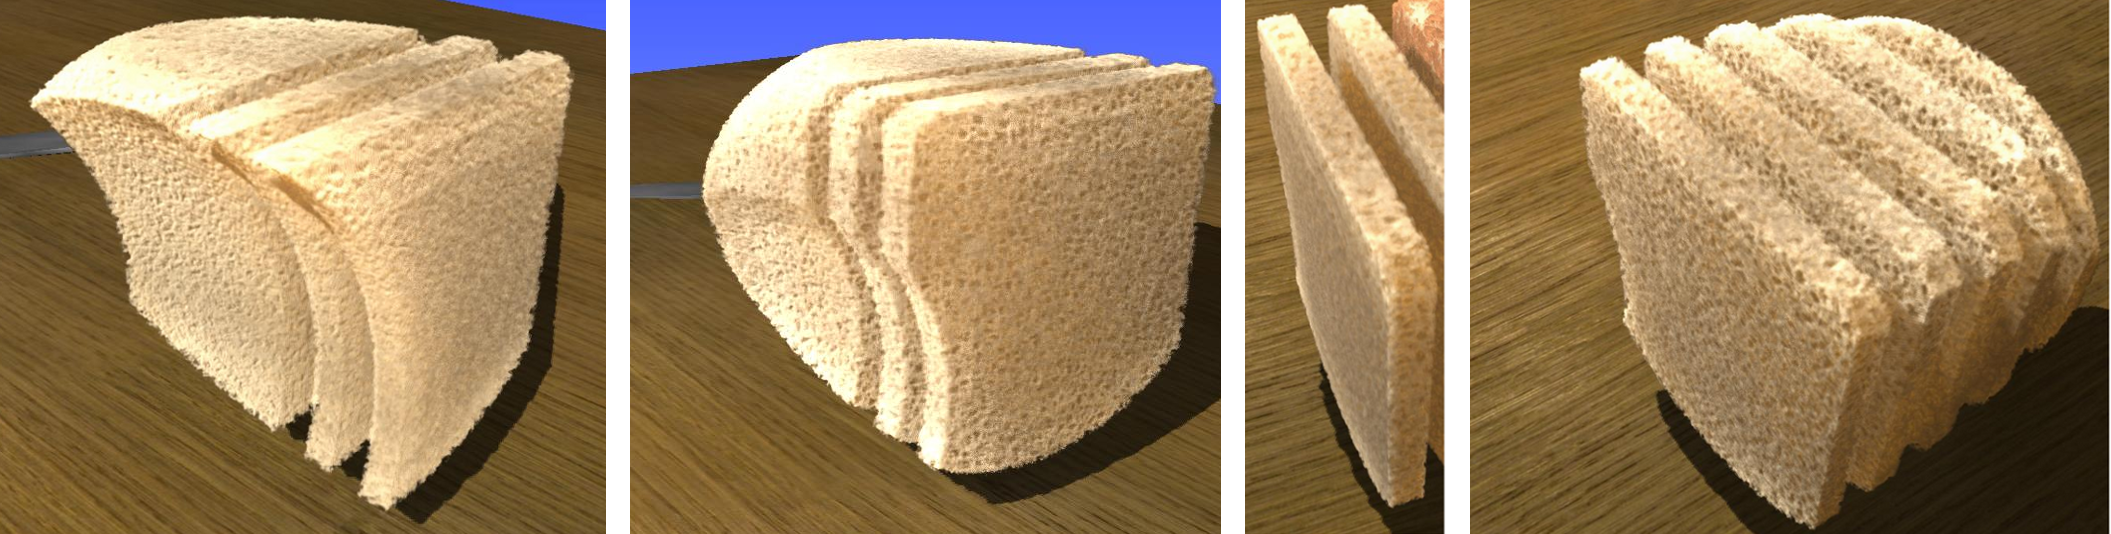
\includegraphics[width=13cm]{figures/crumb}}
  \caption{Miga de pan sintetizada, vista desde distintos ángulos.}
  \label{fg:crumb}
\end{figure}


\begin{figure}
  \centerline{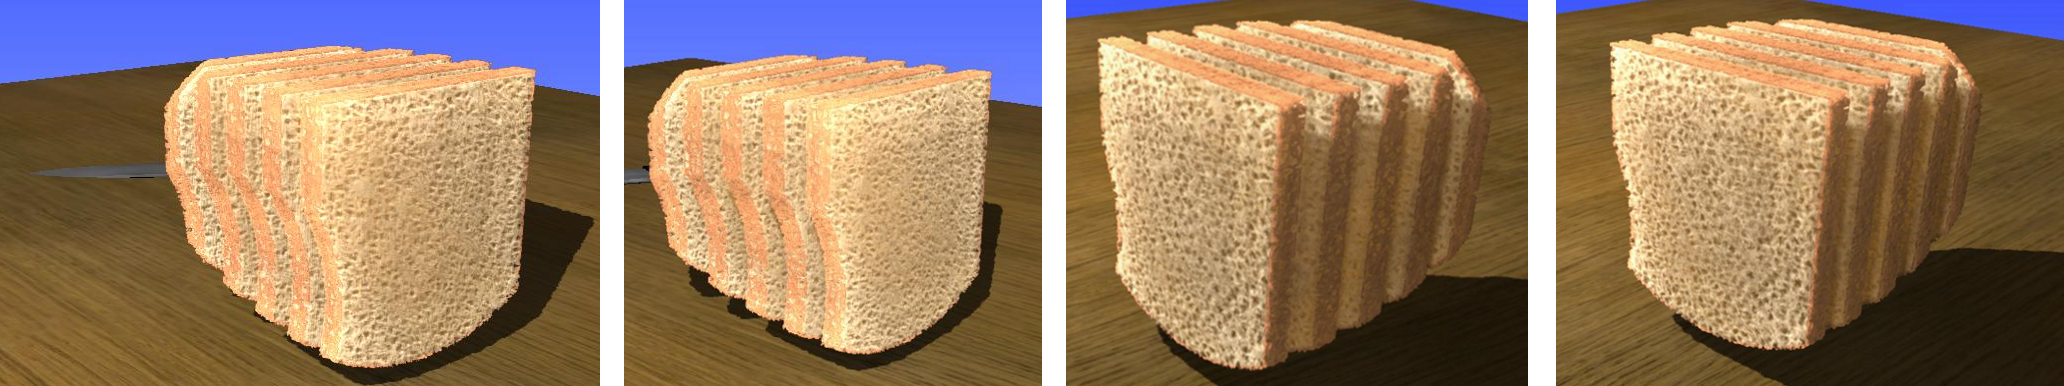
\includegraphics[width=13cm]{figures/results2}}
  \caption{Miga de pan sintetizada, vista desde distintos ángulos (con corteza agregada).}
  \label{fg:results2}
\end{figure}

Si bien es posible la obtención de distintas geometrías de manera sencilla y prácticamente de manera automática, todavía existen limitaciones en cuanto a la flexibilidad de los tipos de pan a producir.
Se depende de un sistema dinámico para producir la forma global de la deformación, pero este sistema es difícil de controlar.
Además, no siempre se adapta de manera sencilla a la forma exterior del material.
Debido a esto, en la siguiente sección presentamos un algoritmo más robusto el cual permite superar estas deficiencias.
El mismo continúa con la idea de la utilización de una definición volumétrica del material, pero el mismo está basado en modelos físicos del proceso de fabricado del pan, extraído directamente de la literatura de ingeniería de los alimentos.

\section{Modelado del Pan desde su Proceso de Fabricación}
Para lograr un modelado realista de la geometría de la miga de pan es necesario comprender su proceso físico de formación.

\begin{figure*}
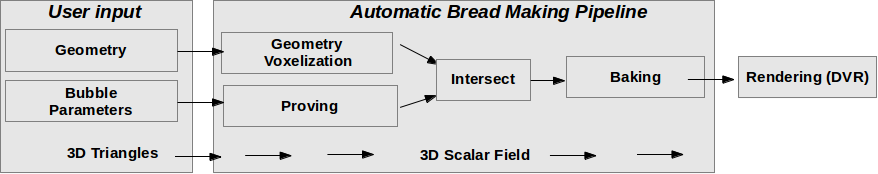
\includegraphics[width=13cm]{figures/pipeline}
\caption{Procedimiento semi-automático para obtener pan sintético foto-realista}
\label{FigPipeline}
\end{figure*}

Utilizando las ideas de la sección anterior, proponemos otro modelo volumétrico de generación de geometrías de migas de pan.
En esta sección proponemos unificar, y diferenciar, los pasos claves presentes en el proceso de fabricación del pan (sobre todo, leudado y cocción).
El procedimiento busca utilizar el proceso físico de generación de geometrías de migas y cortezas de pan a partir de la masa original.
Estos procesos han sido vagamente tenidos en cuenta en la literatura, la cual ha atendido siempre a procesos artísticos más simples, dada la complejidad de los mismos.

En primer lugar, reveeremos el estado del arte del proceso de fabricación del pan.
% e introduciremos modelos matemáticos requeridos para comprender el proceso de cocción.
Luego presentaremos los procesos de modelado, que junto con el modelo de iluminación del siguiente capítulo, permiten obtener imágenes foto realistas de distintos tipos de pan.

\subsection{Trabajo Previo}
El modelado procedimental de geometría reduce fuertemente la necesidad de intervención artística en dominios o situaciones donde la utilización de supervisión repetitiva del proceso se torna impráctica, por ejemplo al modelar ciudades \cite{Parish2001}, planetas \cite{Ebert2002}, edificios \cite{Muller2006}, y plantas \cite{Prusinkiewicz1990}. 
Algunos métodos procedimentales utilizan gramáticas para definir descripciones matemáticas, representando relaciones espaciales entre las primitivas, por ejemplo cubos, cilindros o líneas.
Las estructuras finales usualmente emergen utilizando recursión sobre elementos gramaticales.

Si bien existen algunos ejemplos en la literatura sobre modelado y renderizado de la estructura de migas de pan \cite{Tong2005,Xenakis2007}, los mismos ignoran casi por completo el proceso real de formación.
Algunos trabajos pioneros aplicaron modelos físicos de cocción a determinados tipos de pan para su renderizado, buscando obtener animaciones ({\em e.g.} \cite{Rodriguez-Arenas2011}), pero el modelado de la geometría de las burbujas de la miga del pan no fue tenido en cuenta.

Por otro lado, el modelado procedimental de panes es un tópico multidisciplinario de investigación.
La ingeniería de los alimentos lleva varias décadas de publicaciones en el área, tratando de desarrollar un mejor entendimiento del proceso de formación del pan.
Esta rama de la ciencia muestra que el leudado determina fuertemente las características presentes en la miga de pan, particularmente las burbujas \cite{Babin2006}.
La interacción entre la levadura y algunos nutrientes presentes en la masa produce {\em $CO_{2}$}. 
El radio de las burbujas y sus distribuciones espaciales muestran estructuras con características fractales, exhibiendo autosimilaridad estadística en diferentes escalas de medición.
Determinados trabajos han computado las dimensiones fractales de estas estructuras en determinados tipos de pan \cite{Gonzales2008}, sugiriendo distribuciones fractales uniformes.
El modelado de la cocción del pan es sujeto de numerosos trabajos \cite{Mondal2008}.

El modelado procedimental utilizando fractales también atendió las necesidades de otros variados materiales como montañas \cite{Prusinkiewicz1993}, cráteres lunares, y distribución de las burbujas en quesos \cite{Mandelbrot1983}. 
Adicionalmente, determinados modelos matemáticos complejos representan el comportamiento y el crecimiento de diversos fenómenos naturales.
En computación gráfica, estos modelos son unas de las fundaciones usadas para modelar agua y fluidos \cite{Stam1999,Fedkiw2001}.
Estos trabajos utilizan complejos modelos diferenciales de otras ramas de la ciencia y las aproximan con técnicas numéricas.
En años recientes, la tecnología GPGPU \cite{Owens2007} permitió la posibilidad de alcanzar tiempos reales o interactivos en el cómputo y renderizado de estos modelos numéricos.

A pesar de todos estos avances, el modelado y visualización foto-realista de panes y materiales porosos todavía presenta diversos retos.
Además de un modelo geométrico realista, el renderizado requiere que se represente de manera adecuada los fenómenos de transporte de la luz, incluyendo auto-oclusión, auto-sombreado, transmitancia, translucencia, transparencia, entre otras.
Solamente unas pocas publicaciones proponen atacar ambos problemas, pero utilizando consideraciones artísticas \cite{Xenakis2007}.
Además, estos autores no dan suficientes detalles del modelado y renderización ya que existen derechos de propiedad intelectual, limitando enormemente la reproducción de dichas imágenes.

Por otro lado, la comunidad artística usualmente produce imágenes realistas de pan utilizando fotografías de los mismos, y definiendo geometrías a partir de ellas, junto a la utilización de materiales translúcidos\footnote{http://www.blenderguru.com/tutorials/how-to-create-realistic-bread} y otras consideraciones {\em ad-hoc}\footnote{http://design.tutsplus.com/tutorials/create-a-realistic-loaf-of-bread-in-photoshop--psd-10555}.
Si bien los resultados obtenidos son buenos, los procesos son tediosos y demandan horas.
Además, si se requiere más de una imagen, es necesario repetir todo el proceso desde el principio, lo que torna al mismo muy poco práctico.
Existen numerosas desventajas además de esta.
Por ejemplo, no es posible obtener cortes arbitrarios del material resultante.


\subsection{Visión global del Proceso}
La Fig.~\ref{FigPipeline} muestra el proceso completo de formación de geometrías sintéticas de pan.
Todos los pasos se aplican sobre campos escalares.
Los usuarios pueden proveer el sistema con un modelo de tres dimensiones de su preferencia, o dejar que el sistema provea un pan de forma estándar ({\em croissants}, {\em baguettes}, etc.).
La geometría introducida se voxeliza para proceder a las siguientes etapas.
En la simulación del proceso de leudado, el usuario puede parametrizar la textura del pan (cantidad y tamaño de las burbujas y su distribución), o nuevamente dejar que el sistema provea parámetros estándar que producen tipos de pan conocidos.
La masa cruda será intersectada con la geometría voxelizada para obtener un campo escalar, el cual tiene la forma externa que provee el usuario (o el sistema), con el interior de la misma compuesta de las burbujas procedentes de los parámetros establecidos (ver Sección~\ref{breadprov}).
Luego, se computa un modelo de cocción específico \cite{Powathil2004} para deformar el campo escalar (y las burbujas de éste), de acuerdo a los efectos que produce la cocción en el proceso de formación del pan.
El último paso aplica renderizado directo de volúmenes (direct volume rendering, DVR) \cite{Kruger2003} al campo escalar resultado de la cocción, obteniendo imágenes realistas del pan resultante.

%====================================================================

\subsection{Voxelización de la Geometría}

En nuestro modelo es posible generar panes con geometrías arbitrarias, supliendo un modelo de triángulos en algún formato estándar.
El modelo consta de un conjunto de pasos. El primer paso de la secuencia voxeliza un modelo provisto por un usuario con la utilidad de código abierto {\tt binvox} \footnote{http://www.cs.princeton.edu/~min/binvox/} \cite{Nooruddin2003}.
La voxelización genera un campo escalar binario, con $1$ representando que el voxel dado está dentro de la geometría, y $0$ significando que el voxel está fuera de la geometría.
El paso de leudado (siguiente subsección) genera la textura del material que se ubica dentro de esta geometría voxelizada.
Esto permite generar panes con formas arbitrarias, tales como {\em baguettes}, {\em croissants}, {\em lactal}, u otros menos comunes (una tetera o un conejo).

Un sub-producto importante de la matriz de geometría es un campo escalar secundario que puede ser obtenido por medio de una transformación de distancia.
La transformación de distancia genera una matriz $n$-dimensional con las mismas dimensiones que la matriz que se transforma \cite{osh03}.
La transformación computa, para cada entrada distinta de cero en la matriz, la distancia más cercana a una entrada nula de dicha matriz.
Dada una matríz $n$-dimensional $M$, el algoritmo genera una matriz a valores reales $DF_{M}[i]$ con las mismas dimensiones que $M$,


$$  DF_{M}[i] = \min \bigg\{ \delta(i,j): M[j] = 0 \bigg\},$$

%\begin{align*}
%M'[i] &= min(d(i,j)), M[i] != 0, M[j] = 0\\
%M'[i] &= 0, M[i] = 0,
%\end{align*}

\noindent
donde $\delta(i,j)$ podría ser la distancia de Manhattan o la distancia Euclideana en un espacio $n$ dimensional.
Las entradas de la matriz lejanas a los bordes del objeto tomar valores más altos que aquellas cercanas a los mismos.
De esta manera se obtiene un mapa de la distancia de cada voxel a las superficies tridimensionales del objeto.
Este campo escalar de distancias será requerido en etapas posteriores del proceso.


\subsection{Simulación del Leudado}
\label{breadprov}
Como fue establecido, la textura observable en la masa cruda del pan está compuesta de burbujas, cuya distribución exacta es el resultado de procesos complejos, entre ellos, reacciones químicas, y deformaciones físicas de la masa.
El paso de leudado consta en primera instancia del crecimiento libre de las burbujas, producido por seres vivos, la levadura.
Luego, el cocinero interviene la masa deformándola de diversas maneras.
Finalmente el paso de cocción produce la textura y distribución de burbujas finales.
Los estudios fenomenológicos de estas texturas utilizan tomografía de rayos X y extracción de características sobre las mismas \cite{Gonzales2008,Babin2006,VanDyck2014}.
Buscando obtener una variabilidad similar, en esta tesis generamos distribuciones de burbujas con un modelo basado en fractales, inspirado en las distribuciones de burbujas presentes en el queso, y la textura inducida por los cráteres lunares, propuesto en \cite{Mandelbrot1983}.
Luego validamos los mismos utilizando el método multifractal denominado {\em Sandbox} (caja de arena, ya que realiza cálculos sobre una distribución de puntos aleatoria en la geometría).
Esto será explicado en profundidad en el capítulo de validación.

La textura de la masa es creada procedimentalmente en un campo escalar separado, definido en una matriz de tres dimensiones, de una manera similar a la matriz de geometría en la Subsección arriba.
Cada voxel es iniciado a $1$ (significando que el material aún no tiene burbujas).
El proceso comienza substrayendo esferas de radio $r_{min}$ posicionadas arbitrariamente en el campo escalar (esto se logra seteando a $0$ las celdas respectivas).
Luego, substraemos esferas de radio mayor, nuevamente en posiciones arbitrarias, hasta un radio máximo $r_{max}$.
La relación entre el número de esferas $N_{s}$ a ser sustraídas en cada paso, y sus respectivos radios $r$, está dada por la ley fractal,


\begin{equation*}
N_{s} = \frac{k}{r^{d}},
\end{equation*}

donde $d$ es el exponente fractal que modela la ocurrencia de esferas en relación con su radio, y $k$ controla la cantidad de esferas para cada radio.
Con estos simples parámetros basta para modelar una gran cantidad de texturas en general, particularmente pan.

La Fig.~\ref{FigProving} muestra un ejemplo de un corte en dos dimensiones de este modelo.
Si bien las burbujas esféricas resultantes no son completamente realísticas debido a su forma, los resultados muestran un notorio parecido en tamaños y distribución de tamaños con binarizaciones de cortes reales de masas leudadas (ver \cite{Babin2006}).
Durante la cocción, el campo escalar resultante será sometido a deformaciones geométricas. Consecuentemente, la textura final se ajustará aún más a burbujas de panes reales.
Finalmente, en la sección de validación se buscarán parámetros de generación que ajusten diferentes panes reales. 

\begin{figure}
\center

\includegraphics[width=7cm]{figures/bubbles}
\caption{Simulación Fractal del Leudado de Pan.}
\label{FigProving}
\end{figure}

Luego de la voxelización y la simulación de leudado, las burbujas deben estar presentes sólo en el interior de la geometría.
Para esto, intersectamos ambos campos escalares utilizando un simple producto punto a punto, es decir, una máscara,

\begin{equation*}
P_{2} = P_{1} * G,
\end{equation*}
%
donde $P_{1}$ es el campo $3D$ (matriz) que contiene las burbujas del leudado, y $G$ es el campo escalar que representa a la geometría voxelizada.

La Fig.~\ref{fg:intersectProblem} muestra una versión renderizada de esta intersección.

\begin{figure*}
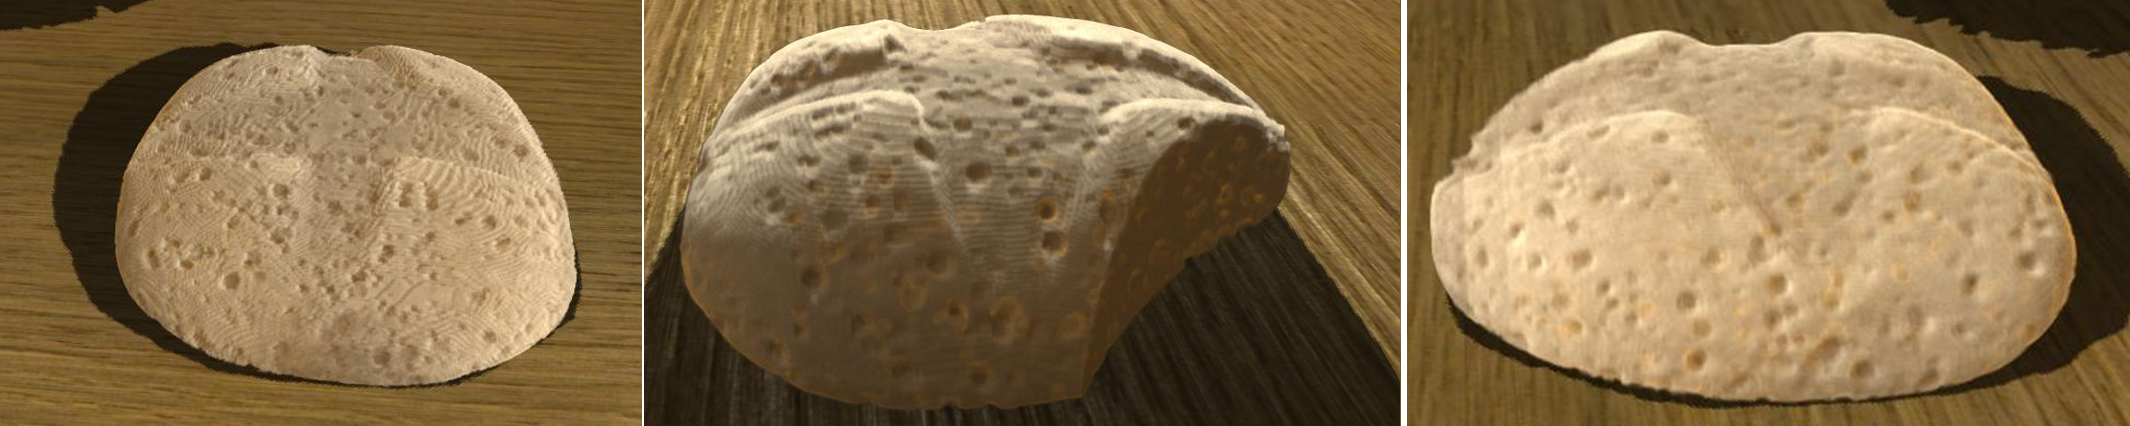
\includegraphics[width=13cm]{figures/intersectProblem}
\caption[Intersección simple de la geometría y de las burbujas provenientes del leudado]{Intersección simple de la geometría y de las burbujas provenientes del leudado. A diferencia de masas reales, pueden verse burbujas en la superficie de la masa.}
\label{fg:intersectProblem}
\end{figure*}

Si bien los resultados pueden parecer realistas, en panes reales, no es habitual que las burbujas sean visibles en la superficie, debido al leudado y cocción reales.
Para solucionar este problema, utilizamos el campo escalar de distancias que computamos previamente, para deshabilitar la generación de burbujas en zonas cercanas a los bordes de la geometría, de acuerdo a cierto valor umbral, el cual será un parámetro.
El campo escalar binario resultante se computa de la siguiente manera,

%\begin{align*}
%DF    &= distField(G),\\
%interior &= DF > umbral,\\
%masa &= G - interior*(1-P_{2}),
%\end{align*}
%
%donde $DF$ es el campo escalar de distancias a la superficie, computado a partir de la geometría de entrada, voxelizada, y $umbral$ es un parámetro que determina el ancho de la región exterior, donde no pueden crearse burbujas.
%Computamos la masa final substrayendo las burbujas ($1-P_{2}$) de la geometría original, pero limitada a la región {\em interior} que acabamos de definir.
Las Figs.~\ref{fg:proving} y \ref{fg:provingBunny} muestran resultados de limitar las interacciones de burbujas a la región interior de la geometría original, donde se observa que no existen burbujas en la superficie de la masa, como ocurre en masas reales.
Las imágenes muestran que el método definido es capaz de producir imágenes realistas de panes crudos con formas arbitrarias.
Cabe remarcar que el modelo es lo suficientemente flexible, permitiendo renderizar el material en cualquier etapa de su proceso de fabricación, además de poder realizar cortes arbitrarios del mismo.

\begin{figure*}
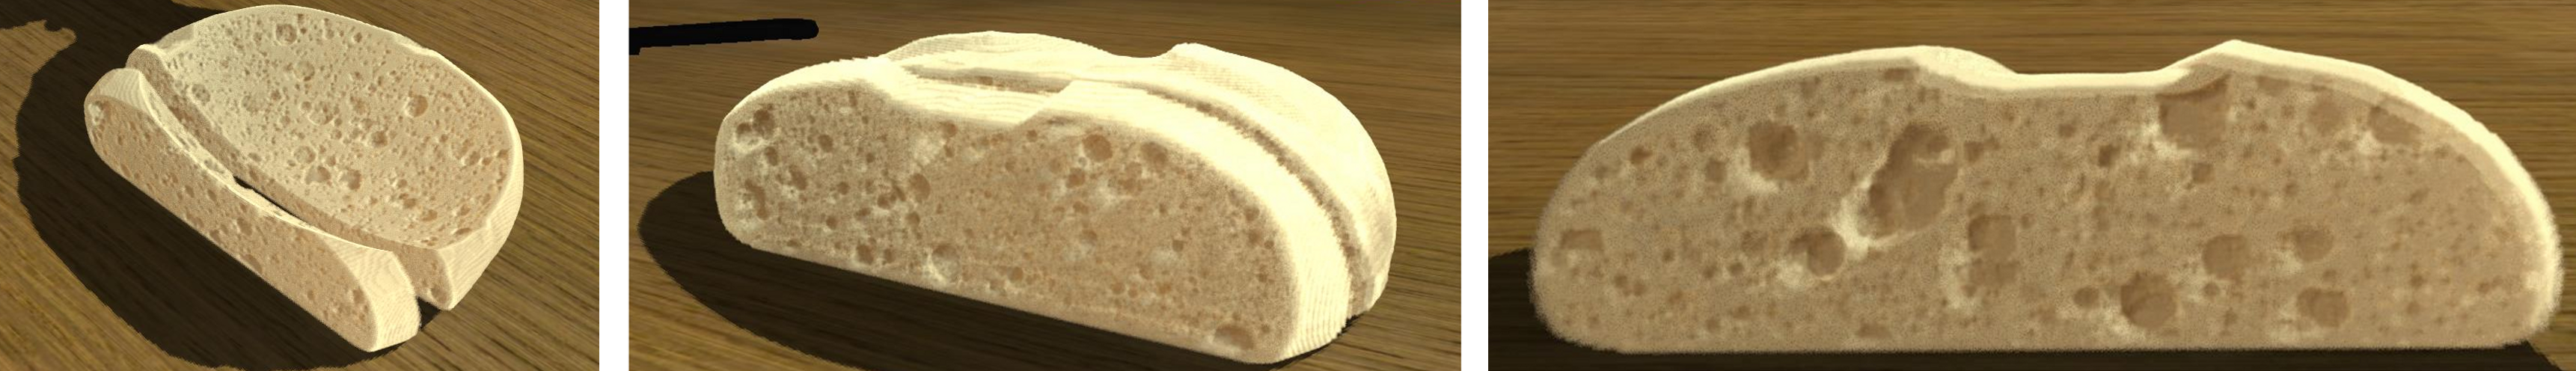
\includegraphics[width=13cm]{figures/prebakebread}
\caption{Pan sintético luego del leudado, y antes de la cocción.}
\label{fg:proving}
\end{figure*}

\begin{figure*}
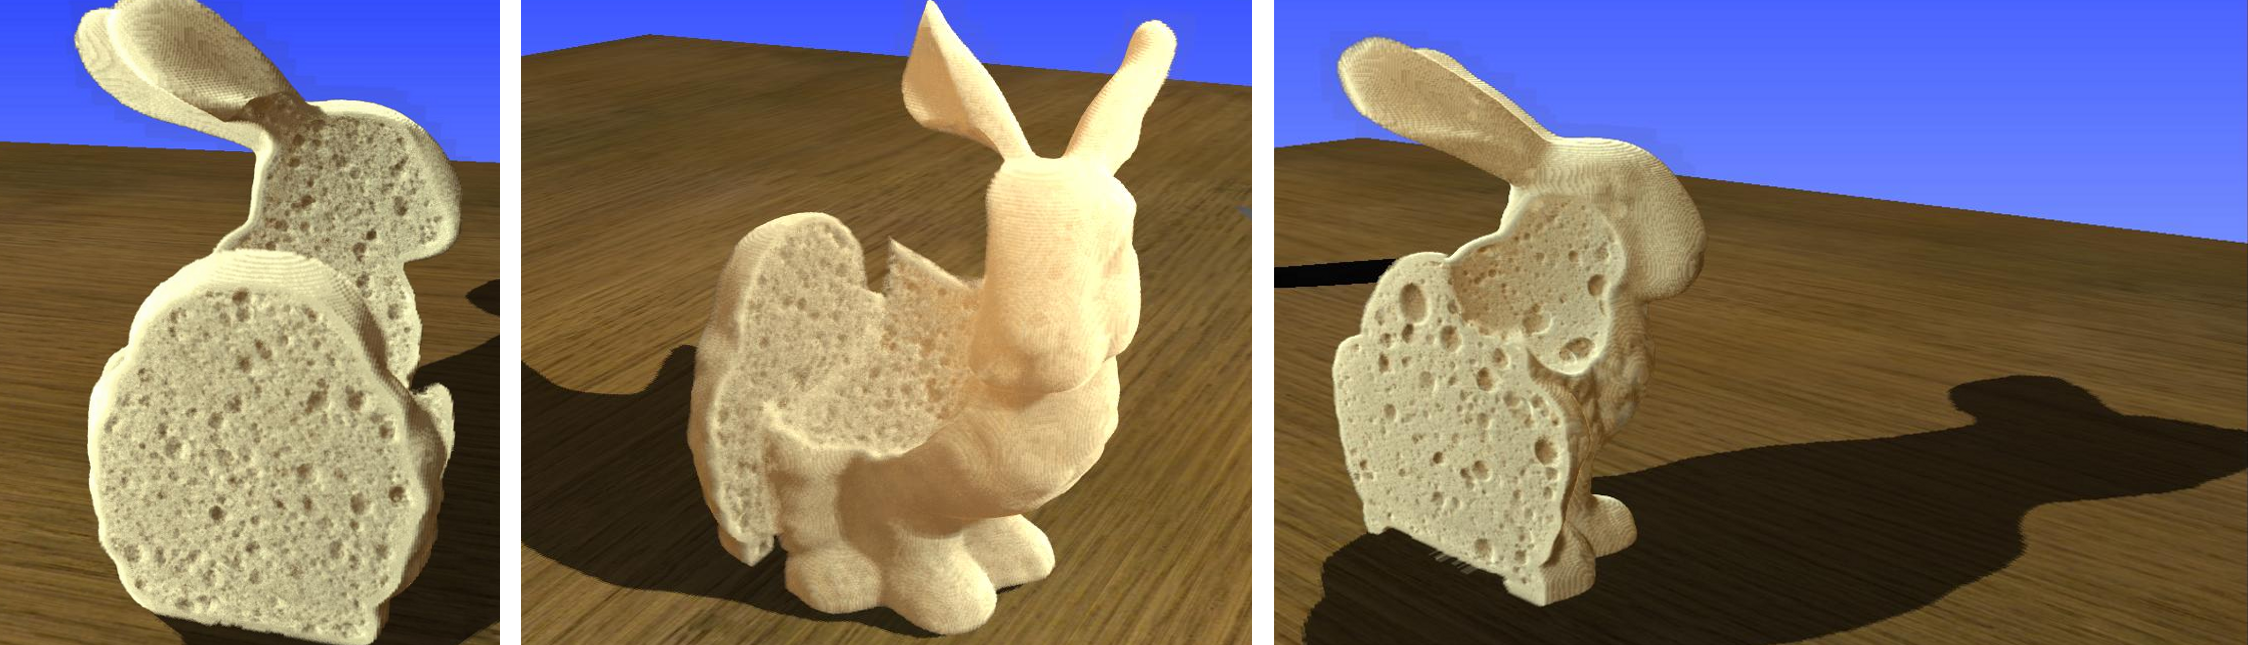
\includegraphics[width=13cm]{figures/prebakebunny}
\caption{Conejo de pan sintético, luego del leudado, y antes de la cocción.}
\label{fg:provingBunny}
\end{figure*}

%====================================================================
\subsection{Cocción}
%To adequately simulate the bread baking process, mathematical models should be able to accurately model the heat and mass transfer in dough.
Los modelos matemáticos del proceso de cocción del pan deben ser capaces de modelar correctamente las transferencias de calor y masa en el mismo.
Los modelos físicos más completos del proceso producen soluciones precisas a la distribución de temperaturas en la masa durante la cocción.
Sin embargo, estos modelos son usualmente muy complejos para implementar y son muy costosos computacionalmente.
Además, sólo los modelos más complejos toman en consideración la formación de la corteza del pan.
La corteza, por otro lado, aún carece de una definición formal~\cite{Vanin2009}.
Por lo tanto, los modelos antes citados incluyen sólo una simplificación de la formación de la misma, muy lejos de lo que ocurre en la cocción real.

Los resultados más relevantes en la literatura sugieren que un modelo unidimensional de la cocción puede ser suficiente para la mayoría de los casos prácticos.
Por ejemplo, Purlis~\cite{Purlis2011} modela la cocción del pan como un problema unidimensional, representando la geometría como un cilindro infinito.
Otros trabajos asumen sólo una coordenada radial, resultando también en modelos $1D$~\cite{Powathil2004, Thorvaldsson1999}.
Estos trabajos muestran que utilizar una representación de una única dimensión produce resultados casi idénticos a aquellos que se obtienen utilizando un mayor número de dimensiones, ya que el efecto de la cocción en las burbujas es la menos importante en el proceso de fabricación del pan.

La simulación numérica que implementamos está basada en el esquema de diferencias finitas propuesto por Powathil~\cite{Powathil2004}, y Thorvaldsson y Janestead~\cite{Thorvaldsson1999}. 
El sistema presentado consiste de un conjunto de tres ecuaciones acopladas que describen transferencia de calor, difusión de varpor de agua y difusión de agua líquida.
En nuestro algoritmo, sólo utilizamos las temperaturas ($T$) como entrada para las siguientes etapas de la formación del pan.
La Ec.~\ref{Eq:heat} modela transferencia de calor en la masa del pan, tomando en consideración el balance de energía y evaporación del agua debido a la temperatura~\cite{Thorvaldsson1999},
%
\begin{equation}
\label{Eq:heat}
\frac{\partial T}{\partial t} = \frac{1}{\rho C_{p}} \frac{\partial}{\partial x} \left ( k \frac{\partial T}{\partial x} \right ) + \frac{\lambda}{C_{p}} \frac{\partial W}{\partial t}+\frac{\lambda W}{ \rho C_{p} }\frac{\partial \rho}{\partial t},
\end{equation}
%
donde $T$ es la temperatura, $x$ es la coordenada radial, $t$ es el tiempo, $C_{p}$ el calor específico, $\rho$ la densidad, $k$ la conductividad térmica, $\lambda$ es el calor latente de la evaporación de agua, y $W(x,t)$ es el contenido de agua líquida. 
Las condiciones iniciales
%
\begin{align*}
T(x,0) &= T_{0}(x), 0\le x \le L/2,
\end{align*}
y las condiciones de borde (continuidad y suavidad) definen el modelo,
\begin{align*}
\left ( \frac{\partial T}{\partial x} \right )_{x=L/2} &= 0 , t > 0 \\
-k \left ( \frac{\partial T}{\partial x} \right )_{x=0} &= h_{r}(T_{r}-T_{s}) + h_{c}(T_{air}-T_{s}) - \lambda \rho D_{w} \left (\frac{\partial W}{\partial x} \right )_{x=0}
\end{align*}
%
donde $h_{r}$ y $h_{c}$ son subtérminos del coeficiente de transferencia de calor ($h = h_{r}+h_{c}$), $T_{air}$, $T_{s}$, $T_{r}$ son temperaturas en el aire circundante, en la superficie del pan, y en la fuente de radiación, respectivamente, $L$ es el alto del pan($x = L/2$ es el centro del pan y $x = 0$ es el contorno del mismo), $D_{w}$ representa la difusividad del agua líquida, y $T_{0}$ la temperatura inicial. 
Las temperaturas están expresadas en Kelvin ($K$). 
El modelo consta de ecuaciones similares para la difusión del vapor de agua ($W$) y difusión de agua líquida ($V$).
Otros detalles del modelo pueden ser consultados en \cite{Thorvaldsson1999}.
En nuestro trabajo, utilizamos este modelo para obtener un mapa de temperaturas al final del proceso de cocción.
Estas temperaturas afectarán posteriormente las formas y tamaños de las burbujas.

La simulación de la cocción define el horno a una temperatura típica (por defecto utilizamos $210^{\circ}C$) y discretiza el tiempo en intervalos $\Delta t = 30s$.
De la simulación se obtiene un arreglo $Temp$, de tamaño $N_{grid}$, compuesto por valores de temperatura.
Por estabilidad numérica, utilizamos $N_{grid}=32$ (como en el trabajo original) e interpolamos las temperaturas para obtener mayores resoluciones ($N_{int}$). 
%Each value represents a dough position after $M$ baking time steps. 

El vector obtenido presenta temperaturas decrecientes de $R = 0$ a $R = L/2$, ya que el centro y el borde del pan poseen la menor y la mayor temperatura, respectivamente, luego de la cocción (el calor fluye desde la corteza hacia el centro del pan). 
Si utilizamos el campo escalar de distancias computado previamente, en conjunto con el vector de temperaturas, podemos mapear distancias a temperaturas.
Esto permite definir temperaturas en el campo escalar de forma compatible a una simulación $3D$.
Basados en estos razonamientos, mapeamos el vector de temperaturas $Temp$ en $3D$ de la siguiente manera,

\begin{equation*}
\displaystyle R(x,y,z) = Temp[ round( DF(x,y,z) ) ], 
\end{equation*}
%
donde $R$ es el campo escalar resultante del mapeo, y $x$, $y$ y $z$ son coordenadas $3D$ en $R$. Cuando $DF(x,y,z) = 0$, la posición actual $3D$ se encuentra en la superficie de la geometría, y $Temp[0]$ se mapea $R(x,y,z)$.
Cuando $DF(x,y,z) > 0$, mapeamos una temperatura menor a $R$, ya que la posición actual se encuentra en el interior de la geometría.
La Fig.~\ref{fg:baking} muestra cortes del resultado de este mapeo ($R$), usando temperaturas resultantes de un tiempo arbitrario de cocción, en los tres planos Cartesianos. 
Las imágenes son casi idénticas a lo que se obtendría con una simulación $3D$~\cite{Purlis2010}.

\begin{figure*}
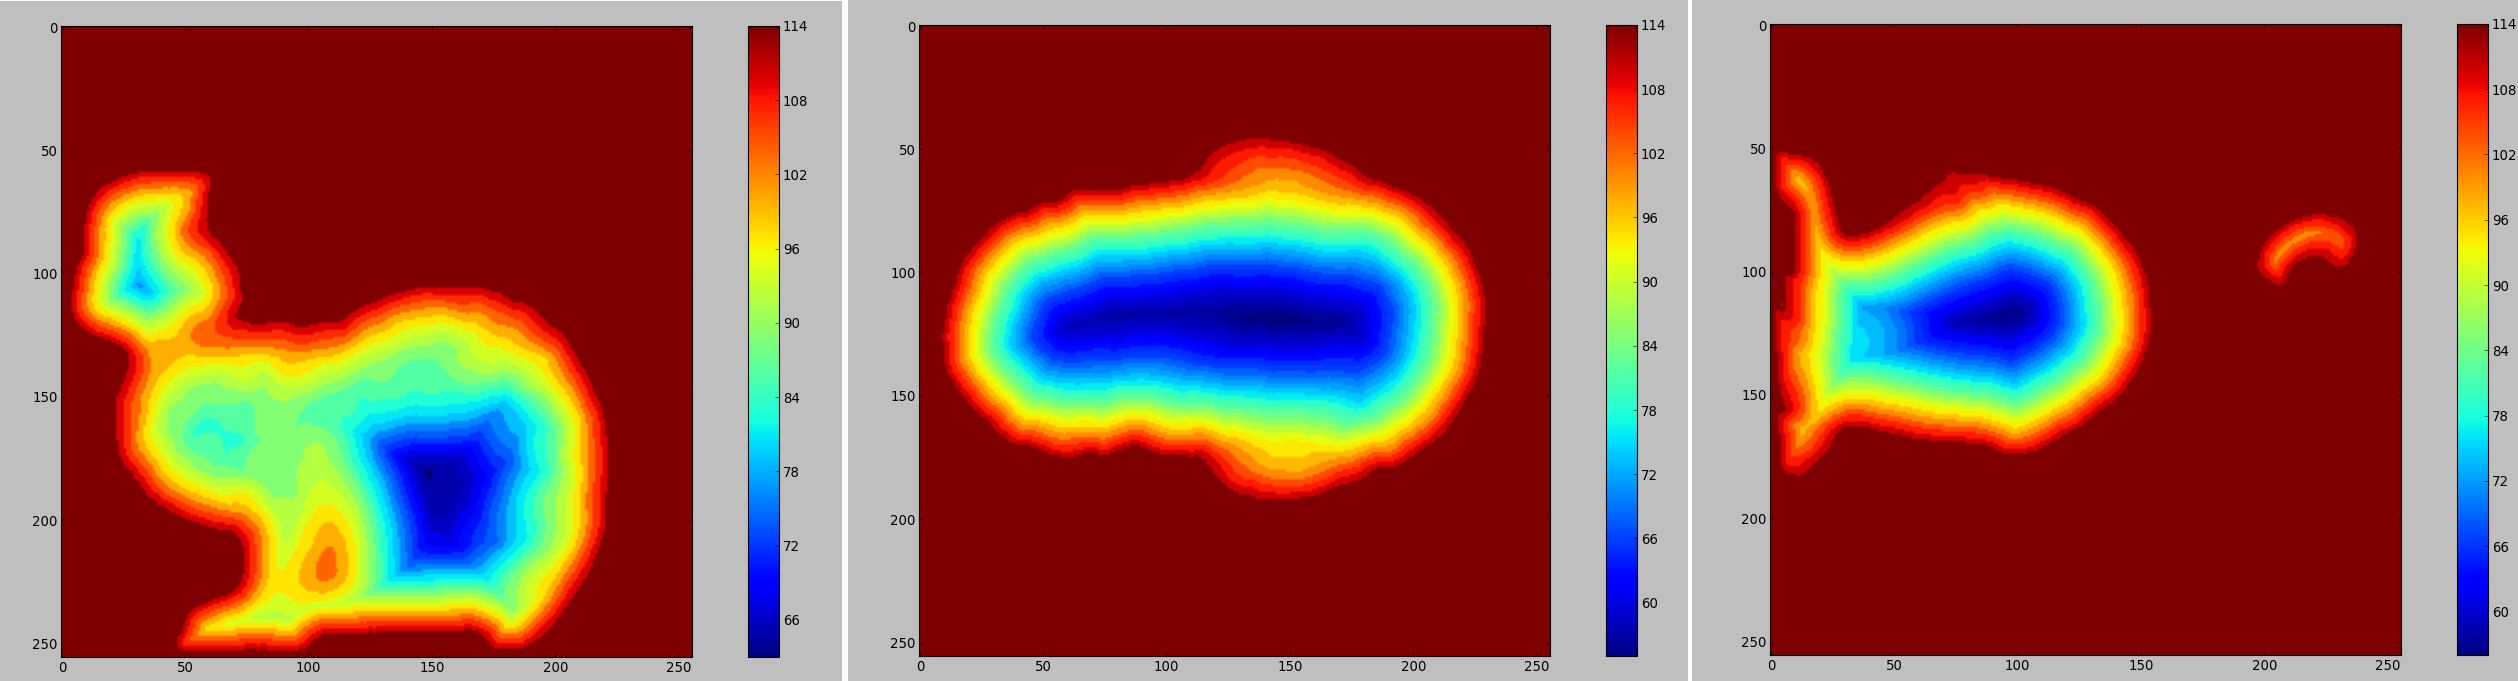
\includegraphics[width=13cm]{figures/tempsbunny}
\caption[Temperaturas unidimensionales mapeadas a un campo escalar tridimensional con forma de conejo]{Temperaturas unidimensionales mapeadas a un campo escalar tridimensional con forma de conejo. Las imágenes muestran que la distribución de temperaturas es similar a una simulación en tres dimensiones.}
\label{fg:baking}
\end{figure*}

Luego de cierto número de pasos de simulación ($t=20$ en nuestro caso), computamos el campo vectorial del gradiente ($g$) de $R$ \cite{Gonzalez2006}, y luego suavizamos el mismo utilizando un kernel Gaussiano.
Finalmente, utilizamos las versiones suavizadas para deformar el campo escalar de la siguiente manera,

\begin{align*}
\displaystyle
u &= x+p*g'_{x}[x,y,z],\\
v &= y+p*g'_{y}[x,y,z],\\
w &= z+p*g'_{z}[x,y,z]
\end{align*}
donde $(u,v,w)$ son las coordenadas en el campo escalar resultante, ($x,y,z$) son las coordenadas originales, $p$ es un parámetro real positivo que denota la intensidad con la que se deforma el campo (controla el efecto neto de la cocción en las burbujas), y las $g'$s son las versiones suavizadas del gradiente original $g$.
%Fig.~\ref{FigBakingVectorField} also shows the computed gradient, where using $[-g_{x},-g_{y}]$ produces a similar vector but in the clockwise direction that can be applied with similar effects on the bubbles. 
La Fig.~\ref{fg:bakedbubbles} muestra cortes $2D$ de campos escalares luego de aplicado el proceso de cocción a diferentes formas.

\begin{figure*}
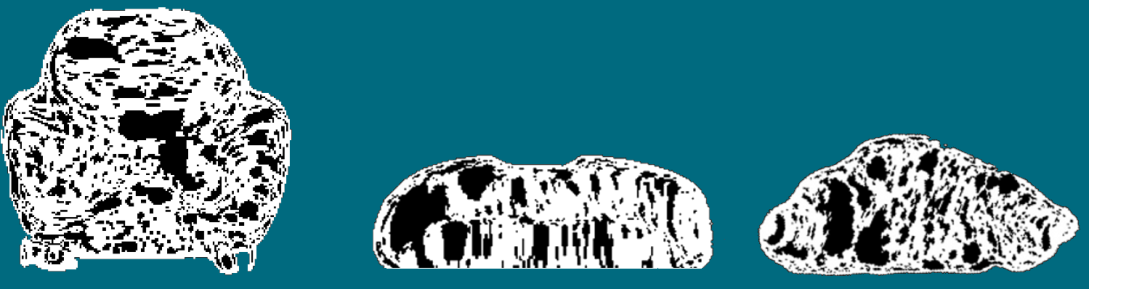
\includegraphics[width=13cm]{figures/bakedbubbles}
\caption{Cortes bidimensionales con burbujas deformadas por el proceso de cocción en diferentes tipos de panes.}
\label{fg:bakedbubbles}
\end{figure*}

El parámetro $p$ puede ser utilizado para sintetizar diferentes apariencias de miga de pan, desde cruda hasta burbujas con mucha deformación (ver Fig.~\ref{fg:parameterp}).
Cuando incrementamos $p$, forzamos a las burbujas a seguir más ajustadamente la forma exterior del pan. 
La imagen también muestra que el método deforma más pronunciadamente las burbujas más cercanas a la corteza.

\begin{figure*}
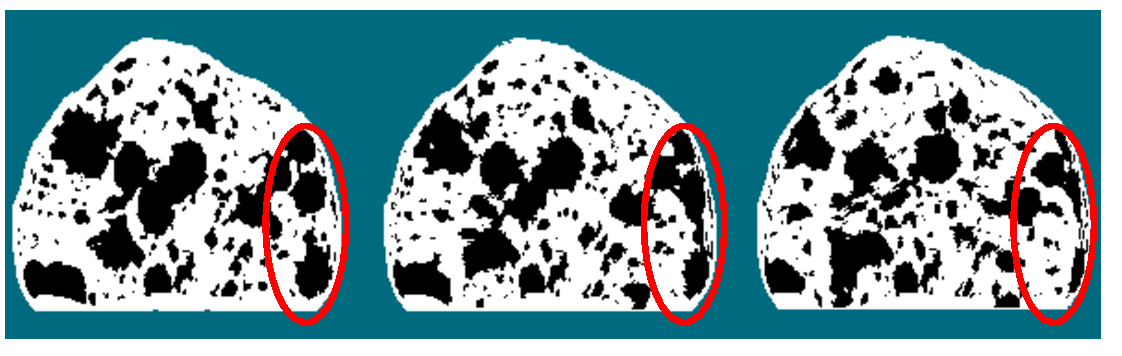
\includegraphics[width=13cm]{figures/parameterp}
\caption[Efecto del parámetro $p$ en la simulación de cocción]{Efecto del parámetro $p$: de izquierda a derecha $p$ es $0$, $5$, $10$,$15$, y $25$, respectivamente.}
\label{fg:parameterp}
\end{figure*}


\subsection{Formación de la Corteza}
El modelo de cocción que hemos introducido no incluye detalles precisos de la formación de la corteza.
En estas ecuaciones, la corteza se asume es producida en la superficie del material, a determinada temperatura, pero esta simplificación está lejana a lo que ocurre actualmente en el proceso real de cocción.
La literatura de ingeniería de los alimentos define la corteza como una interfase que emerge entre la masa y el aire.
Entre sus principales características se encuentra la formación de un material más denso en la superficie, y una diferenciación de color.
Sin embargo, los detalles precisos acerca de cómo esto ocurre se desconocen, por lo tanto, la apariencia exacta de la misma, está lejos de ser comprendida en los modelos presentes acutalmente.

Debido a esto, y basados en la aproximación inicial asumida, utilizamos el campo escalar de distancias computado previamente para definir una región de corteza.
Esta elección está fundada en el hecho de que la corteza está mayormente determinada por un frente de evaporación que resulta de la temperatura \cite{Jefferson2007}.
En otras palabras, obtenemos las posiciones utilizando el campo escalar mencionado, ya que hemos definido una relación entre la temperatura y la distancia a la superficie.
Además, obtenemos diferentes apariencias de pan utilizando un parámetro de distancia que determina diferentes anchos de corteza.

También, por completitud, presentamos otro método para calcular la misma.

\paragraph{Determinación de la corteza utilizando morfología matemática}
Debido a que es difícil o imposible definir funciones matemáticas algebraicas que se adapten a cualquier forma, proponemos un método automático para determinar regiones del volumen utilizando el formalismo conocido como morfología matemática \cite{Gonzalez2001}.

Con esto, se presente obtener una región que se ajuste a los bordes del campo escalar.
Para esto se utilizarán técnicas simples conocidas como apertura, cierre, erosión y dilatación.

Las operaciones las definiremos en campos escalares tridimensionales.
Un elemento estructurante $E$ es un campo escalar binario que representa una forma particular (cubo, esfera, etc.).
Los elementos estructurantes son utilizados en la definición de las operaciones antes mencionadas.
La operación de erosión se utiliza para reducir el tamaño total del campo escalar.
La erosión de un campo escalar $A$ utilizando un elemento estructurante $B$ es definida de la siguiente manera,

\begin{equation}
A \ominus B = \{z\in \mathbb{Z}^3 | B_{z} \subseteq A\},
\end{equation}

\noindent donde $B_{z}$ es la traslación de $B$ por el vector tridimensional$z$.

La dilatación es una operación utilizada para aumentar el tamaño total del campo escalar, siguiendo sus bordes.
La dilatción de un campo escalar $A$ utilizando el elemento estructurante $E$ es definida como sigue,

\begin{equation}
A  \oplus E = \bigcup_{e\in E} A_e.
\end{equation}

La operación de cierre es utilizada para cerrar {\em agujeros} en el campo escalar.
El cierre de un campo $B$ utilizando un elemento estructurante $E$ es definido como una dilatación seguida de una erosión,

\begin{equation}
B \bullet E = (B \oplus E) \ominus E,
\end{equation}

ver \cite{Gonzalez2001} para obtener mayores detalles.

Para obtener la región externa de la geometría representada en el campo escalar, hay que eliminar los agujeros internos que representan las burbujas y luego computar el borde.
Para esto, el primer paso produce un cierre $c$ del campo escalar utilizando un cubo (elemento estructurante de radio $r$), causando el cierre de las burbujas internas.
Llamaremos $d$ a la dilatación de $c$ con un elemento esférico de radio $r_{2}$ y $e$ a la erosión $d$ utilizando un elemento estructurante esférico con un radio ligeramente menor($r_{3}$).
La diferencia entre $d$ y $e$ ($d-e$) se encuentra en el borde del campo escalar, por lo cual puede utilizarse como corteza.
Para eliminar posibles imperfecciones en los pasos anteriores, se suaviza el campo escalar por medio de un cierre de $d-e$ y una dilatación del resultado, obteniendo la corteza final.


La Fig.~\ref{fg:crusts} muestra ejemplos de campos escalares con cortezas agregadas utilizando este técnica. Los resultados se adaptan naturalmente a cualquier campo escalar, inclusive si existen agujeros grandes.
El resultado cubre completamente el campo escalar, por lo cual para poder observar la parte interna del material deben realizarse cortes en el mismo.

\begin{figure}
  \centerline{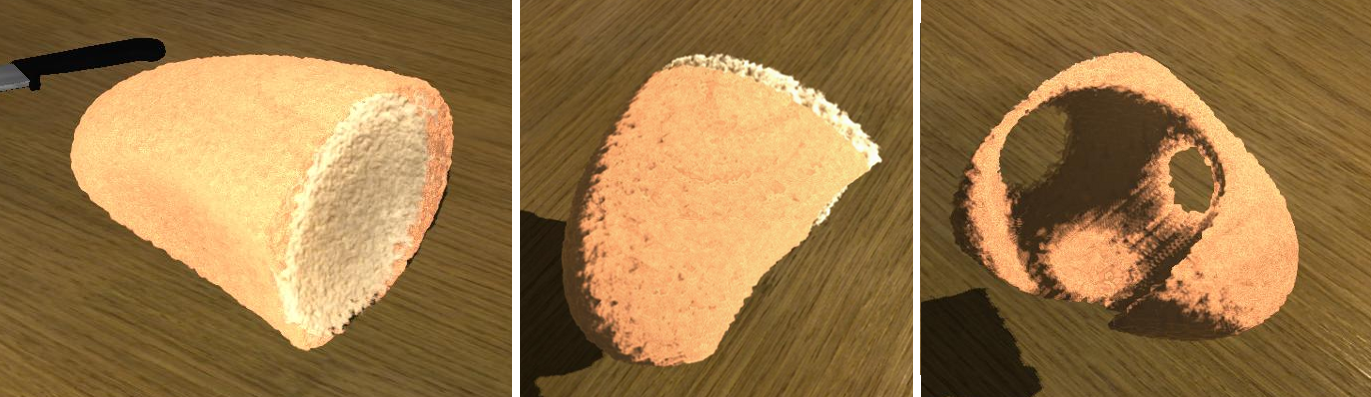
\includegraphics[width=13cm]{figures/crusts}}
  \caption[Determinación de la corteza del pan utilizando morfología matemática]{Determinación de la corteza del pan utilizando morfología matemática. La imagen de la derecha muestra que el método de utilización de morfología matemática funciona incluso cuando existen grandes agujeros en el campo escalar.}
  \label{fg:crusts}
\end{figure}

\subsection{Tiempos de cómputo}
En la implementación utilizamos Python\footnote{python.org} y Cython\footnote{cython.org}.
En la Tabla~\ref{tab:computingtimes} se muestran tiempos de cómputo típicos para los distintos pasos en la simulación de la formación del pan, detallados en secciones anteriores. %In addition, rendering times with DVR are in the order of $~300$ ms (milliseconds), achieving interactive framerates.

\begin{table}[h!]
       % Give a unique label
% For LaTeX tables use
\begin{tabular}{lllll}
\hline\noalign{\smallskip}
Resolución del Campo Escalar & $256^{3}$ & $384^{3}$  & $512^{3}$ \\
\noalign{\smallskip}\hline\noalign{\smallskip}
Leudado & 0.28 & 0.97 & 2.29 \\
Intersección & 8 & 10.81 & 14.97 \\
Campo escalar de Distancias & 7 & 23.73 & 56 \\
Cocción & 19.92 & 51.15 & 117.27 \\
%Rendering & 1s & 4s & 0\% \\
\noalign{\smallskip}\hline
\end{tabular}
\caption{Tiempos de cómputo típicos en nuestro modelo expresados en segundos.}
\label{tab:computingtimes}
\end{table}

Es importante mencionar que la mayor parte del tiempo de cómputo en la cocción está dedicado al cómputo del gradiente, y no al proceso de cocción en sí.
Debido a los costos computacionales en resoluciones superiores, el usuario puede generar vistas previas de los panes utilizando campos escalares con menores resoluciones.


\section{Resultados}
En esta sección presentamos imágenes renderizadas de geometrías de pan obtenidas utilizando nuestro modelo.

Las Figs.~\ref{fg:renders}, \ref{fg:renders2}, y ~\ref{fg:renders3} muestran imágenes renderizadas de panes obtenidos en este trabajo.
Las Figs.~\ref{fg:renders} y ~\ref{fg:renders2} marcan las diferencias en realismo entre resoluciones del campo escalar de ($256^{3}$) y  ($512^{3}$) respectivamente.
La Fig.~\ref{fg:renders3} muestra versiones de alta resolución en el campo escalar de otras geometrías, incluyendo panes con formas de conejos.
La Fig.~\ref{fg:croissant} muestra un pan con forma de {\em croissant} en el cual se han hechos distintos cortes, los cuales demuestran que el método permite obtener imágenes de partes arbitrarias del material.
Las Figs.~\ref{fg:bigalveoli} y ~\ref{fg:bakedbunny} muestran un pan típico y uno con forma de conejo, mostrando burbujas grandes y las burbujas deformadas como resultado del proceso de cocción.
Además se cambió el color de la miga.

Los colores de corteza y miga son parámetros definibles por el usuario. Los cortes en la miga son fácilmente producidos cambiando a $0$ las regiones deseadas en el campo escalar luego de la cocción, y antes del renderizado.

\begin{figure*}[!ht]
\begin{center}
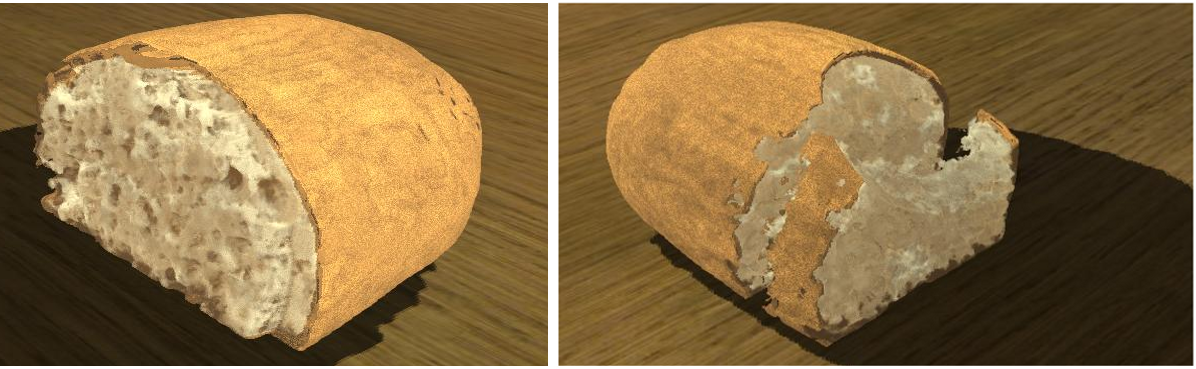
\includegraphics[width=13cm]{figures/otherbread}
\caption[Cortes de pan luego de la cocción, utilizando un campo escalar de dimensiones $256^{3}$]{Cortes de pan luego de la cocción, utilizando un campo escalar de dimensiones $256^{3}$. Las imágenes muestran que la miga y la corteza son consideradas en nuestro modelo.}
\label{fg:renders}
\end{center}
\end{figure*}

\begin{figure*}[!ht]
\begin{center}
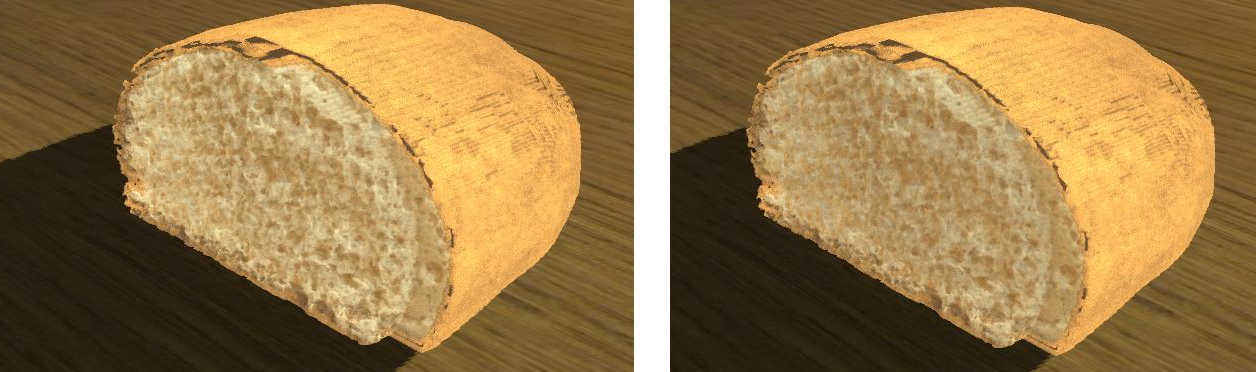
\includegraphics[width=13cm]{figures/otherbread512}
\caption[Cortes de pan luego de la cocción, utilizando un campo escalar de dimensiones $512^{3}$]{Cortes de pan luego de la cocción, utilizando un campo escalar de dimensiones $512^{3}$. Se observan mayores detalles en la miga, lo cual aumenta el realismo de la imagen.}
\label{fg:renders2}
\end{center}
\end{figure*}

\begin{figure*}[!ht]
\begin{center}
\includegraphics[width=13cm]{figures/final}
\caption{Cortes de pan luego de la cocción con distintas geometrías.}
\label{fg:renders3}
\end{center}
\end{figure*}

\begin{figure*}[!ht]
\begin{center}
\includegraphics[width=13cm]{figures/croissant}
\caption[Cortes de una Croissant luego de la cocción]{Cortes de una Croissant luego de la cocción. La imagen muestra el interior de la miga en distintas regiones del volumen.}
\label{fg:croissant}
\end{center}
\end{figure*}

\begin{figure*}[!ht]
\begin{center}
\includegraphics[width=13cm]{figures/baked}
\caption[Cortes de pan luego de la cocción, con burbujas de mayor tamaño]{Cortes de pan luego de la cocción, con burbujas de mayor tamaño, como es típico en determinados panes reales.}
\label{fg:bigalveoli}
\end{center}
\end{figure*}

\begin{figure*}[!ht]
\begin{center}
\includegraphics[width=13cm]{figures/bakedbunny}
\caption[Efecto de la cocción sobre el pan sintético.]{Cortes de pan luego de la cocción con burbujas de mayor tamaño. Además, puede observarse más claramente el efecto de la cocción en la deformación de las burbujas, las cuales tienden a seguir la forma de la corteza.}
\label{fg:bakedbunny}
\end{center}
\end{figure*}

%Images show realistic bread appearances, suitable for photo-realistic rendering and serious ga\-mes \cite{Susi2007}. 


%This is illustrated in Figure~, where arrow lengths indicate vector modulus. The image shows that the field's influence is higher near the crust, mostly deforming outer bubbles. This behavior is consistent with real bread crumbs: baking influences the outer bubbles' shape, elongating them parallel to the crust \cite{Scanlon2001}, in other words, following its isotherms.


%\subsection{Leudado}
%El leudado es el principal responsable de la apariencia visual de las burbujas en la miga de pan \cite{}.

%Los patrones observados en la distribución de las burbujas son resultado de procesos complejos, entre los que encontramos reacciones químicas y deformaciones físicas. Este paso en la fabricación consiste en un crecimiento libre de las burbujas, producido por organismos vivos (levadura) en la masa sin cocción del pan.

%Diferentes estudios fenomenológicos de la distribución de burbujas aparecen en la literatura. Los mismos utilizan tomografía de rayos X y extracción de características sobre imágenes para obtener una imagen y modelar las mismas \cite{Babin2006,Gonzales2008,VanDyck2014}.

%El modelo utilizado está inspirado en un modelo propuesto en \cite{Mandelbrot1983}, el cual intenta modelar quesos y distribuciones de cráteres en cuerpos celestes. Validaremos la distribución obtenida utilizando una métrica multi-fractal basada en el espectro multifractal Sandbox.

%Se comienza con una esfera de radio $v = 1$ voxels. Este radio es incrementado en cada iteración. En cada paso, se extraen un número de esferas proporcional al radio:


%\begin{equation}
%N_{esferas} = \frac{k}{r^{d}},
%\end{equation}

%\noindent donde $k$ y $d$ son parámetros con valores reales, y $r$ es el radio de la esfera.

%La Figura~\ref{FigProving} muestra un ejemplo en dos dimensiones de este proceso, donde $d$ controla la relación existente entre los radios de las esferas y $k$ el número de esferas que extraemos en cada paso.

%Las imágenes muestran una apariencia similar a las que pueden observarse en diferentes espumas (café, jabón, cerveza), y en particular a la que muestra el leudado del pan \cite{Babin2006}. 

%\begin{figure}
%\includegraphics[scale=0.28]{bubbles.png}
%\caption{Fractal bread proving simulation.}
%\label{FigProving}
%\end{figure}

%En la sección de validación ajustaremos los parámetros para adecuarlos a los de imágenes de migas reales de pan.

%\subsection{Cocción}
%\subsubsection{Modelo Matemático}

%El modelo matemático del proceso de cocción simula la transferencia de calor y masa en diversos alimentos, entre ellos el pan.  En esta tesis utilizaremos modelos de una dimensión~\cite{Thorvaldsson1999,Purlis2010}. Por ejemplo, Purlis~\cite{Purlis2010} modela la geometría del pan como un cilindro infinito.

%Utilizaremos la solución numérica presente en {Thorvaldsson and Janestead \cite{Thorvaldsson1999} and Powathil~\cite{Powathil2004}. La misma modela el problema como un conjunto de tres ecuaciones diferenciales acopladas que describen transferencia de calor, difusión de vapor de agua y difusión de agua. Sólo será tenida en cuenta la temperatura ($T$) como entrada en el pipeline de generación de pan.
%The paper defines the geometry as a prism of dimensions $12\times12\times2~cm^{3}$, with  $x$ (the shortest side) as the coordinate of interest.


%La siguiente ecuación modela la transferencia de calor en la masa de pan a través de un balance de energía y de evaporación de agua debido a la temperatura~\cite{Thorvaldsson1999}:
%
%\begin{equation}
%\frac{\partial T}{\partial t} = \frac{1}{\rho C_{p}} \frac{\partial}{\partial x} \left ( k \frac{\partial T}{\partial x} \right ) + \frac{\lambda}{C_{p}} \frac{\partial W}{\partial t}+\frac{\lambda W}{ C_{p} \rho}\frac{\partial \rho}{\partial t}
%\end{equation}
%
%donde $T$ es la temperatura, $x$ ies la coordenada radial, $C_{p}$ es calor específico, $\rho$ es la densidad, $k$ es la conductividad térmica, $\lambda$ es el calor latente de evaporación de agua, y  $W(x;t)$ es el contenido de agua líquida. Las condiciones iniciales:
%
%\begin{align}
%T(x,0) &= T_{0}(x), 0\le x \le L/2
%\end{align}
%y las condiciones de borde completan el modelo:
%\begin{align}
%\left ( \frac{\partial T}{\partial x} \right )_{x=L/2} &= 0 , t > 0 \\
%-k \left ( \frac{\partial T}{\partial x} \right )_{x=0} &= h_{r}(T_{r}-T_{s}) + h_{c}(T_{air}-T_{s}) - \lambda \rho D_{w} \left (\frac{\partial W}{\partial x} \right )_{x=0}
%\end{align}
%
%donde $h_{r}$ y $h_{c}$ son subtérminos del coeficiente de transferencia de calor ($h = h_{r}+h_{c}$), $T_{air}$, $T_{s}$, $T_{r}$ son las temperaturas en el aire, en la superficie del pan y en la fuente de radiación, respectivamente, $L$ es la altura del pan ($x = L/2$ es el centro del pan y $x = 0$ es el borde del pan), y $T_{0}$ es la temperatura inicial. Las temperaturas se expresan en Kelvin ($K$).  Además el modelo presenta ecuaciones similares para la difusión de vapor de agua ($W$) y la difusión de agua líquida ($V$). Más detalles del modelo pueden ser encontrados en \cite{Thorvaldsson1999}.

%Utilizamos este modelo para obtener un mapa de temperaturas sobre el volumen del pan al final del proceso de cocción. Estas temperaturas se utilizarán para deformar la geometría de las burbujas resultantes del proceso de leudado.



%El modelo matemático del proceso de cocción es un modelo $3D$ que, en su versión más simple involucra transferencia de calor y de masa.

%El proceso de creación de pan real sitúa a la cocción luego de la deformación de la masa. Esto supone geometría arbitraria en los bordes de la masa. El proceso de cocción debe amoldarse a estas condiciones arbitrarias, lo cual hace que el modelo resulte complejo. Para simplificar esto, proponemos aplicar la cocción antes de deformar la masa original. Esta simplificación resulta adecuada para nuestros propósitos y es validada posteriormente.


%Además, para nuestros propósitos la inclusión de un modelo completo $3D$ resulta excesiva dado su costo computacional y el limitado impacto final sobre la estructura que pretendemos modelar. Por estas razones elegimos un modelo cilíndrico unidimensional, el cual se extiende fácilmente a $3$ dimensiones. A pesar de esta simplificación, la literatura muestra que el modelo captura los detalles esenciales en la transferencia de calor y masa \cite{Purlis2010,Powathil2004}.

%La implementación numérica del modelo está descrita en \cite{Powathil2004}. La misma usa el esquema de diferencias finitas. El horno en el cual se sitúa el pan se establece a $210  ^{\circ}C$ y el tiempo es discretizado en intervalos de tiempo de duración $\Delta t = 0.05s$. El algoritmo devuelve un arreglo $Temp$ de $N_{grid}$ valores de temperatura. Cada valor representa una posición en la masa luego de $M$ pasos temporales. Por cuestiones de estabilidad definimos el tamaño de la grilla como $N_{grid}=32$ e interpolamos los valores de temperatura para obtener mayores resoluciones ($N_{im}$).

%El vector obtenido presenta temperaturas decrecientes de $R = 0$ a $R = L/2$, debido a que el centro del pan presenta las menores temperaturas ($R=L/2$), a diferencia de los bordes ($R=0$) los cuales poseen una distancia menor a la fuente de calor. De esta manera, $Temp[L/2]$ corresponde a $x = N_{im}/2, y=N_{im}/2$ y $Temp[0]$ corresponde a los $(x,y)$ lejos del centro del cilindro. 

%Luego de interpolar las temperaturas traducimos el vector $Temp_{int}$ a coordenadas $2D$ mediante las siguientes relaciones:
%\begin{align}
%\displaystyle I(\frac{N_{im}}{2}-i,\frac{N_{im}}{2}-j) &= Temp_{int}[L/2-R], \\
%R &= \sqrt{i^{2}+ j^{2}}, \\
%i, j &\in [-\frac{N_{im}}{2},\frac{N_{im}}{2}],
%\end{align}


%\noindent donde $R$ es el índice del vector, y $x$ e $y$ son coordenadas $2D$ en la imagen de destino, en otras palabras, el píxel $I(N_{im}/2-i,N_{im}/2-j)$ es seteado con el valor $Temp_{int}[L/2-R]$. Finalmente obtenemos una imagen cuadrada de lado $N_{im}$. La figura ~\ref{FigBakingVectorField} muestra un ejemplo de dicha imagen.

%A partir de esta imagen obtenemos su gradiente \cite{Gonzalez2006} para  computar un campo vectorial $[g_{x},g_{y}]$, utilizándolo para deformar posteriormente la textura volumétrica de la siguiente manera:

%\begin{align}
%\displaystyle u = x+p*dist_{xy}*g_{x}[x,y],\\
%v = y+p*dist_{xy}*g_{y}[x,y],
%\end{align}
%\noindent donde $(u,v)$ son las coordenadas en el volumen deformado, ($x,y$) son las coordenadas originales, $p$ es parámetro real positivo que sirve para modular el efecto del campo en el volumen, y $dist_{xy}$ es la distancia euclídea de $(x,y)$ al centro del cilindro ($\sqrt((x-N_{x}/2)^{2}+(y-N_{y}/2)^{2})$). 


%El parámetro distancia al centro es útil para remarcar las diferencias existentes en el efecto que produce el proceso de cocción sobre las burbujas en distintas zonas de la masa.
%La Figura~\ref{FigBakingVectorField} muestra además el vector gradiente superimpuesto sobre la imagen. En nuestros experimentos encontramos que $p=10$ es suficiente para producir un efecto apreciable sobre las burbujas.
%El procedimiento de cocción reduce aproximadamente a la mitad el tamaño total de la imagen.



%\begin{figure}
%\centering
%\includegraphics[scale=0.58]{vfield.png}
%\caption{Temperaturas obtenidas sin interpolar a partir del modelo matemático de cocción del pan y vector gradiente superimpuesto}
%\label{FigBakingVectorField}
%\end{figure}

%El largo de las flechas indica el módulo del vector. La imagen muestra que la influencia del campo es mayor cerca de la corteza del pan, lo cual se condice con el efecto observable en panes reales. El proceso de cocción elonga paralelamente a la corteza las burbujas del material \cite{Scanlon2001} (siguiendo las isotermas).

%Siguiendo el modelo cilíndrico, cada rodaja (representada por un volumen de altura $1$ vóxel) es deformado independientemente utilizando el mismo procedimiento. La Figura~\ref{FigBaking} muestra un ejemplo de rodaja luego de la cocción digital.

%Cabe mencionar que se intentó interpolar la imagen resultante en lugar del vector original de temperaturas, pero el campo vectorial resultante tenía vectores de módulos cercanos a cero.

%\begin{figure}
%\begin{center}
%\includegraphics[scale=0.8]{baking.png}
%\caption{Corte del volumen luego de la cocción. Las burbujas siguen un campo vectorial concéntrico.}
%\label{FigBaking}
%\end{center}
%\end{figure}


%\subsection{Intervención Humana en el Proceso}

%\subsubsection{Mean Value Coordinates}

%Para permitir una interacción con el modelado del pan sintético, se definen puntos de control que el usuario puede mover a voluntad para deformar localmente la masa. Para esto se utiliza Mean Value Coordinates (MVC), el cual es un método poderoso en animación \cite{Floater2003,Floater2005,Ju2005}.
%Este método computa coordenadas baricéntricas a partir de los puntos de control sin deformar (una caja que rodea al objeto) con las cuales calcula las posiciones destino de los puntos de interés en el dominio (en nuestro caso, cada pixel de la imagen es un punto de interés).

%El método usa dos conjuntos de puntos de control para realizar la deformación. El primero ($cageOrig$) es un conjunto de puntos que se sitúa en el borde de la imagen original. Cada texel computa su coordenada baricéntrica con respecto a estos puntos. Cuando movemos estos puntos formamos el vector $cageNew$. Para cada píxel $(x,y)$ el método computa las coordenadas baricéntricas del mismo con respecto a la caja original, multiplicando las mismas con los puntos de control deformados. El resultado $(u,v)$ se utiliza como coordenadas en la imagen original para setear el valor que debe tomar el píxel actual:
%\begin{align}
%barycoords &= bary([x,y],cageOrig),\\
%(u,v) &= \sum_{i} {barycoords_{i} * cageNew_{i}}, \\
%T_{new}(x,y) &= T_{orig}(u,v).
%\end{align}
%As the reader will see in next sections, this method produces realistic-looking deformations.

%====================================================================

%Durante el proceso de fabricación del pan, la masa sufre transformaciones que incluyen la intervención del ser humano, el cual busca distribuir la levadura de manera homogénea por medio de deformaciones.

%En nuestro modelo, permitimos que un artista pueda definir puntos de control en una imagen para modificar la silueta externa de la masa. Siguiendo el modelo cilíndrico, la deformación en esta etapa se aplica a cada corte $2D$ del volumen.

%La Figura~\ref{FigMVC} muestra un ejemplo de deformación utilizando Mean Value Coordinates. En este caso se necesitaron solamente $11$ puntos de control (rojo) para aproximar la silueta de la corteza. La FIgura~\ref{FigMVCpoints} muestra los puntos de control y la caja deformada En el ejemplo definimos un mayor número de puntos de control en la región de interés (derecha) para producir una silueta más controlada.

%\begin{figure}[!ht]
%\includegraphics[scale=0.65]{warping.png}
%\caption{Comparación entre pan real (izquierda) y sintético utilizando la deformación por MVC (derecha).}
%\label{FigMVC}
%\end{figure}


%\begin{figure}[!ht]
%\includegraphics[scale=1.35]{warppoints.png}
%\caption{Imagen deformada utilizando MVC: puntos de control sin modificar (verde) puntos de control modificados (rojo). Otras líneas indican desplazamiento de puntos. }
%\label{FigMVCpoints}
%\end{figure}


%This method also warps the bubbles' shape. The deformed bubbles have a natural appearance in concordance with real bread bubbles. 
\section{Conclusiones}
En este Cap\'itulo hemos introducido diversos algoritmos para subsanar la falta de procedimientos flexibles e intuitivos para modelar determinados materiales, entre ellos materiales porosos como el pan. Además, como subproducto de la investigación, se obtuvieron representaciones bidimensionales de madera, granito, mármol y otros materiales comunes en la literatura.
Hemos demostrado visualmente la capacidad de los métodos.

El primer aporte es un algoritmo que produce texturas bidimensionales de materiales conocidos como madera y granito, utilizando sistemas de partículas, el cual fue presentado en una conferencia local \cite{Baravalle2011}.

Haciendo hincapié en materiales porosos, particularmente el pan, diseñamos algoritmos que utilizan sistemas de partículas en conjunción con Sistemas Dinámicos para producir texturas que representan de manera realista geometrías de pan, el cual fue presentado en un congreso y revista nacionales \cite{Baravalle2014}.

Finalmente, utilizando como referencia el proceso de formación real del pan, utilizamos conocimientos de ingeniería de los alimentos para producir una secuencia de pasos que emulan el proceso real de formación del pan.
El mismo permite modelar de manera realista tipos de panes arbitrarios, produciendo geometrías de su miga y su corteza, utilizando un proceso fractal de generación.
Para ello, emulamos un proceso de leudado configurable por el usuario, tanto en forma global, supliendo una geometría arbitraria en tres dimensiones, como en el burbujeado interno, por medio de parámetros intuitivos de generación (radio máximo y mínimo de las burbujas, cantidad de burbujas, etc.).
Luego aplicamos una simulación física de la cocción que deformó ligeramente las burbujas.
Finalmente, la corteza fue generada sobre la superficie del material.
El algoritmo de renderizado utilizado será explicado en el siguiente capítulo, el mismo produjo imágenes realistas de diversos tipos de pan, en varias etapas del proceso de formación del mismo.

El modelo introducido es más flexible y poderoso que el estado del arte actual en modelado de geometría de materiales porosos y panes.

En un capítulo posterior, y con intención de validar el procedimiento, mostraremos que las geometrías obtenidas por el método inspirado en el proceso de formación del pan, arrojan distribuciones de burbujas coincidentes con panes reales.

 \cleardoublepage

\chapter{Renderización de Geometrías Porosas}
\section{Introducción}
Debido a las limitaciones existentes actualmente en el renderizado realista de geometrías porosas en tiempos interactivos, nos proponemos en este capítulo estudiar la utilización de renderizado directo de volúmenes (Direct Volume Rendering, \acrshort{DVR} \cite{Kratz2006}), aplicado a un campo escalar representando la geometría del material. 
Los resultados obtenidos son realistas y se renderizan en tiempo real. La misma evita el uso de estructuras intermedias, simplificando el desarrollo y reduciendo los costos computacionales.

El renderizado foto-realista de materiales con una estructura interna compleja presenta grandes retos en computación gráfica.
En particular, los materiales porosos son translúcidos y complejos, presentando detalles dispares en distintas escalas, todos igualmente necesarios de ser tenidos en cuenta para lograr una correcta visualización.
El renderizado realista de estos materiales debe simular correctamente diversos fenómenos como translucencia, auto-sombreado, auto-oclusión, reflectancia, y absorción, entre otros.

Las técnicas del estado del arte en renderizado de materiales porosos tratan el material como una superficie, capturando sus propiedades por medio de un complejo procedimiento en el cual la luz reflejada por el material se fotografía desde distintos ángulos.
Posteriormente la información se procesa y reconstruye para formar un modelo del material.
Si bien esta solución captura adecuadamente los fenómenos lumínicos previamente discutidos, también es cierto que la practicidad del método se encuentra severamente comprometida, presentando un elevado costo computacional, un procedimiento de captura muy limitado y la imposibilidad de obtener más de una apariencia con una única captura.

En un intento por superar estas limitaciones, proponemos utilizar la técnica de DVR, la cual implementamos en \acrshort{GPU}, utilizando el lenguaje de shader GLSL (ver Apéndice A).
La técnica permite renderizar los campos escalares computados en el capítulo anterior sin utilizar estructuras intermedias.
Las imágenes obtenidas son promisorias, y se computan en tiempo real gracias al poder de las placas gráficas actuales.

\section{Trabajo Previo}
El tópico de renderizado foto-realista de materiales, y su modelado, atrajo un interés creciente en la literatura científica.
La mayoría de los esfuerzos están focalizados en materiales complejos de frecuente aparición como el agua \cite{Schechter2012}, la piel humana \cite{Donner2006}, metales, plásticos \cite{Kurt2010}, etc.
La comunidad de investigadores, sin embargo, ha tenido grandes dificultades para simular adecuadamente la apariencia de otros materiales, como en el caso de materiales cocidos ({\em e.g.}, pizza, galletitas).
Debido a su compleja geometría y fenómenos lumínicos involucrados, esto continúa siendo un problema abierto \cite{Voglsam2013}.

En los últimos años, el costo computacional de renderizar modelos físicos de estos materiales resultaba prohibitivo si el tiempo real era un requerimiento.
De todas formas, el crecimiento notable en poder de cómputo debido al diseño masivamente paralelo de las placas gráficas \cite{Yeo09,Harris06}, está permitiendo la simulación de fenómenos complejos de interacción de la energía radiante con materiales en tiempos de cómputo aceptables.

%Simular un modelo geométrico aceptable representa un reto adicional, como fue visto en el capítulo anterior.
%El pan y otras estructuras porosas son el resultado de mecanismos complejos que involucran deformaciones físicas, transferencia de masa y calor durante la cocción, y distintas reacciones químicas.

Estudios recientes utilizan consideraciones fenomenológicas sobre materiales porosos, pero la geometría resulta invariable (es decir, no procedimental) \cite{VanDyck2014}: una geometría fija no permite obtener diferentes tipos de pan fácilmente, ya que requiere un procedimiento de captura para cada uno de ellos.
Adicionalmente, las distribuciones de burbujas no pueden ser controladas.

La presencia de mesoestructuras (burbujas con formas complejas) provocan una clasificación de los materiales porosos como {\em cuasi-homogéneos} \cite{Tong2005}. 
Por esta razón, modelar al material como una superficie no resulta adecuado.
Técnicas típicas como BRDFs, BSSRDFs \cite{Donner2009} y BTFs, no resultan satisfactorias.
Una publicación intenta resolver las limitaciones \cite{Tong2005}, pero las desventajas que acarrea (proceso de captura muy complejo, altos costos computacionales, invariabilidad geométrica), resultan en un proceso basado en fuerza bruta y muy poco práctico.

\section{Renderizado Directo de Volúmenes (DVR)}

La técnica de DVR genera imágenes bidimensionales computando la interacción de la luz con un medio semi-transparente, el cual se representa a través de un campo escalar discreto.
Este campo describe la densidad del medio en cada celda discretizada.
Para cada píxel en la imagen final, se computa un rayo desde la posición de la cámara en el espacio virtual, y la radiancia que alcanza la cámara desde esa dirección se computa aproximando la RTE en su forma integral, ec. (\ref{eq:rteintegral}).
Esta ecuación describe la modificación de radiancia a medida que el rayo atraviesa el medio no transparente.
En su forma completa, la RTE incorpora muchas propiedades ópticas y efectos.
Para aproximar el resultado de la RTE en tiempo real, este capítulo utiliza una versión simplificada de la ecuación que sólo toma en consideración algunos de los fenómenos ópticos que ocurren en la realidad.

Como fue explicado en el Capítulo $2$, existen tres fenómenos ópticos importantes que afectan la propagación de la luz a través de un medio en un punto dado del espacio: emisión, absorción, y dispersión.
La emisión se define como la generación de energía radiante en una dirección dada.
La absorción ocurre cuando una fracción o toda la energía radiante en el rayo de luz se topa con un objeto opaco transformándose en otras formas de energía.
Finalmente, la dispersión produce modificaciones de dirección en los fotones.
Aquellos eventos que provocan que los fotones modifiquen su dirección a otra distinta a la dirección del rayo, son llamados de dispersión saliente. Del mismo modo, los eventos que provocan que los fotones modifiquen su dirección por la del rayo actual se llaman dispersión entrante.

%
La contribución de la dispersión entrante en la radiancia se computa a partir de una única dirección, la cual corresponde a la principal fuente de luz de la escena.
Esto aproxima la energía radiativa que llega a un punto desde la fuente de luz, haciendo rebotar a las partículas en el medio hacia ese punto y luego viajando a lo largo de una dirección dada. 

La RTE puede reescribirse a partir de la ecuación (\ref{eq:rteintegral}), para ser utilizada en DVR como sigue,

\begin{equation} \label{eq:general_radiance}  
  L(p_n) = L_b + \int_{p_0}^{p_n} \frac{\partial L(t)}{\partial p} \, dt,
\end{equation}

\noindent donde $L_b$ es la radiancia de fondo, y $p_0$, $p_n$ son los puntos visibles más cercano y más lejano en la dirección del rayo, respectivamente, $L(t)$  es la radiancia en el punto $t$, y $\partial p$ es la distancia entre puntos consecutivos muestreados. 
Debido a que la entrada del algoritmo de DVR constituye un conjunto de datos discreto, la integral en $L(p_n)$ se aproxima por una suma.

La extinción constituye el descenso de radiancia en un rayo debido a absorción y dispersión saliente.
Podemos aproximar este efecto definiendo un coeficiente de absorción para el medio, $k_a$ y un coeficiente de dispersión saliente $k_s$. 
Si descartamos el efecto de dispersión saliente, la fórmula que describe la radiancia alcanzando un punto luego de atravesar un segmento de un rayo es:

\begin{equation} \label{eq:radiance_absorption}  
    L_b \ e^{- \textstyle  \int_{p_0}^{p_n} k_a(t) \, dt}.
\end{equation}

Introducimos el valor $\int_{p_i}^{p_j} k_a(t) \, dt$, el coeficiente de absorción, el cual referiremos como $\tau_{(p_i, p_j)}$. 
La transmitancia representa el concepto complementario a la extinción, describiendo la cantidad de luz que escapa a un medio en una dirección dada.
Por lo tanto, el valor de la transmitancia entre dos puntos $p_i$ y $p_j$ es:

\begin{equation} \label{eq:transmittance}  
  T(p_i,p_j) = e^{- \textstyle \tau_{(p_i, p_j)}}.
\end{equation}

Asumiendo un incremento en la radiancia en cada punto del rayo dentro del volumen, dada por la dispersión entrante y fenómenos de emisión ($\rho$), luego nuestra estimación inicial de radiancia resulta,

\begin{equation} \label{eq:ray_radiance}  
  L(p_n) = L_b \ e^{-\tau(p_0, p_n)} + \int_{p_0}^{p_n} \rho \ e^{-\tau(t,p_n)} \, dt.
\end{equation}

Esto significa que la radiancia a lo largo de los puntos $p_0$ y $p_n$ es la radiancia de fondo atenuada, más la emisión y la dispersión entrante atenuadas en cada punto del rayo.

El algoritmo de DVR muestrea la función de densidad del volumen a intervalos regulares, aproxima la transmitancia a lo largo de esos puntos y computa la cantidad de luz que llega a la cámara a lo largo de la dirección del rayo.
La computación reemplaza la suma integral por una suma discreta sobre el rayo intersectando el volumen,

\begin{equation} \label{eq:ray_radiance}  
  L(p_n) = L_b \ e^{-\tau(p_0, p_n)} + \sum_{p_0}^{p_n} \rho \ e^{-\tau(p_i,p_n)}.
\end{equation}

Es posible tener en cuenta otros efectos, aumentando la fidelidad de la imagen final, así como los costos computacionales de la técnica.
La base de nuestro algoritmo de renderizado utiliza un modelo simplificado que sólo tiene en cuenta transmitancia $T$, emisión constante y dispersión entrante $\rho$ (aproximada a través del cómputo de la radiancia desde cada punto hacia la luz), junto con ciertas consideraciones artísticas, para alcanzar tasas de refresco de tiempo real.
Describiremos el algoritmo de renderizado en detalle en una sección posterior.

\section{Implementación}

Se creó una aplicación demo\footnote{disponible en \emph{https://www.github.com/rbaravalle/Pysys}}  que usa el sistema de partículas descrito en secciones previas para renderizar panes en tiempo real, utilizando DVR.
La Fig.~\ref{fg:application} muestra la aplicación desarrollada, con un objeto poroso renderizado en tiempo real.
En la demo se produce una textura volumétrica, renderizando un cubo que corresponde a esta textura en la escena.
El material utilizado para renderizar el cubo consta de un shader de vértices muy simple, y un shader de fragmentos, el cual implementa el algoritmo de DVR.
Para cada fragmento, el shader computa un rayo con origen en la posición de la cámara y con la dirección del fragmento que debe ser coloreado.
El procedimiento muestrea la textura volumétrica a intervalos regulares sobre la intersección del rayo y el cubo.
Estos valores muestreados son luego utilizados como entrada de un algoritmo que implementa la Ec. (\ref{eq:ray_radiance}), computando el color del píxel resultante de la manera descrita en secciones previas.



\begin{figure}
\centerline{\includegraphics[width=11cm]{figures/application}}
\caption{Aplicación desarrollada mostrando una estructura porosa renderizada en tiempo real.}
\label{fg:application}
\end{figure}


La implementación acumula la transmitancia a lo largo del rayo y la contribución de radiancia en cada punto muestreado.
La computación termina si el valor de la transmitancia acumulada está por debajo de un umbral (lo cual significa que no escaparán más fotones en el rayo) o si el rayo sale del cubo.
La dispersión entrante ($\rho$), simplificada, se computa a través de un rayo secundario, para cada punto muestreado, en dirección a la fuente de luz.
Este rayo secundario se muestrea para determinar la cantidad de luz que llega al punto.
Esta técnica permite obtener sombras naturales dentro del volumen.
El píxel se sombrea utilizando la información de transmitancia del rayo primario y los secundarios en cada punto.
En este punto, diferentes consideraciones artísticas pueden ser aplicadas para obtener diferentes materiales con distintos aspectos.
Por ejemplo, podemos diferenciar miga de corteza asignando un coeficiente de extinción mayor y un color más oscuro a las regiones de corteza.
En nuestro caso, se aplica un color amarillo suave en ciertas regiones, otorgándoles una apariencia de miga.
Adicionalmente se puede agregar una sutil reflexión especular.
Para esto, se necesita computar la primera intersección entre el rayo y la geometría.
Gracias a esto se puede incrementar ligeramente el realismo final de la imagen.
El vector normal usado en este cálculo está dado por el gradiente de la textura volumétrica en ese punto.

La demo presentada provee al usuario la habilidad de modificar parámetros como el coeficiente de absorción, el umbral de transmitancia, los colores asignados y la visibilidad de los reflejos especulares.
Con la modificación de estos parámetros, el usuario puede producir imágenes que semejan distintos materiales porosos, como las esponjas, budines, panes o piedras.
La Fig. \ref{fg:fragmentshaderrte} muestra un esquema del shader de fragmentos implementado, donde se computa la Ec. (\ref{eq:ray_radiance}).

\begin{figure}[htb!]
\centerline{\includegraphics[width=9cm]{figures/fragmentshader}}
\caption[Cálculo de color en el shader de fragmentos]{Cálculo de color en el shader de fragmentos. Se implementa la suma en la ecuación (\ref{eq:ray_radiance}). La suma devuelve un color que luego se colorea por medio de un parámetro del usuario. Además, luego se computarán las normales, sombras y oclusión de ambiente.}
\label{fg:fragmentshaderrte}
\end{figure}


\subsection{Oclusión Ambiente}

La aproximación introducida a la RTE no tiene en cuenta fenómenos clave en la obtención de imágenes realistas, como la dispersión entrante y la dispersión saliente.
Sin embargo, un aspecto clave para resaltar la apariencia de la imagen final está basada en las contribuciones locales de radiancia debido a características microscópicas propias del material.
Hasta ahora, la dispersión entrante, simple, era aproximada por medio del cómputo de la radiancia entrante en el punto desde la fuente de luz.
Es posible lograr aproximaciones más precisas tomando en consideración además la dispersión entrante al punto desde el medio, por medio del agregado de la oclusión ambiente.
La literatura muestra que considerarla produce imágenes de mayor realismo \cite{Hernell2010}.

Debido a estas consideraciones proponemos computar la dispersión entrante, múltiple, calculando de manera offline un término de oclusión del ambiente para cada voxel en el campo escalar y almacenándolo como una textura volumétrica extra, la cual se suple al shader de fragmentos, permitiendo así mantener los tiempos computacionales en tasas razonables.
Para cada voxel en la textura volumétrica resultante de alguno de los métodos del capítulo anterior, el cómputo de dicho término define un radio $r$, almacenando el valor medio de los voxels vecinos dentro de una esfera que contiene ese radio.
Luego, este valor se utiliza para modular la contribución de cada paso del rayo.
Experimentalmente encontramos que variar el valor de $r$ produce resultados visualmente indistinguibles, por lo cual cualquier valor mayor que $0$ puede utilizarse para el cómputo.
La Fig.~\ref{fg:occlusion} muestra el realce que produce este concepto, resultando en un aspecto clave de nuestra implementación, a la hora de producir imágenes creíbles. 



\begin{figure}
\centerline{\includegraphics[width=10cm]{figures/occlusion}}
  \caption[Pan renderizado sin y con oclusión de ambiente]{Pan sin (izquierda) y con (derecha) oclusión de ambiente. La imagen final se realza notablemente, apreciándose una apariencia más natural.}
  \label{fg:occlusion}
\end{figure}
 
\subsection{Cómputo de las Normales}
El gradiente en el punto será utilizado para computar el vector normal en el modelo de iluminación.
Utilizamos un esquema {\em hacia adelante} en el cómputo de diferencias finitas del gradiente, el cual resulta de la diferencia normalizada, entre la posición {\em hacia adelante} y la posición actual del campo escalar,


\begin{equation}
\begin{aligned}
x &= tex(pos+\vec{i}) - tex(pos)\\
y &= tex(pos+\vec{j}) - tex(pos)\\
z &= tex(pos+\vec{k}) - tex(pos) \\
N &= normalizar([x,y,z])
\end{aligned}
\end{equation}

\noindent donde $\vec{i}$, $\vec{j}$ y $\vec{k}$ son los vectores unitarios que forman una base en $\mathbb{R}^{3}$.

La normal y el vector que representa la fuente de luz permiten determinar la contribución especular en el punto, aplicando un modelo de Phong con un exponente suave, y estableciendo un parámetro que permite al usuario especificar el impacto deseado para la componente especular.
Se han testeado otros modelos especulares más complejos, pero no se encontró diferencia apreciable en la apariencia final de la textura de pan.

\subsection{Cómputo de Sombras}
La técnica de DVR puede ser utilizada para computar sombras realistas, desde el objeto renderizado hacia la escena en la que se encuentra, por medio de mapas de sombras \cite{Williams1978}.
Durante la generación del mapa de sombras renderizamos nuevamente un cubo representando la geometría, pero esta vez los cómputos se realizan desde la posición de la fuente de luz.
El shader de fragmentos para ese cubo utiliza el mismo método de rayos explicado, pero solo computa la transmitancia en el rayo.
Si la transmitancia en ese rayo está por encima de un umbral al finalizar el cómputo (lo cual significa que cierta cantidad de fotones logran escapar al medio), luego el fragmento no corresponde a un oclusor, y su profundidad se establece a infinito.
Si durante el cómputo de la transmitancia, la misma cae por debajo del umbral, la profundidad del fragmento se establece en la profundidad alcanzada por el rayo en ese momento.

A partir de este cómputo obtenemos un mapa de sombras, el cual puede almacenarse como una textura.
Luego se computa DVR normalmente (desde el punto de vista del observador).
En este paso debe mapearse cada texel del mapa de sombras con una posición en el espacio, para determinar si el punto está en sombra o no.
Esta técnica se utiliza junto a un filtrado de porcentaje de cercanía, para generar sombras realistas en nuestra aplicación.
Casi todas las imágenes presentadas muestran el uso de esta técnica en nuestra aplicación.


\subsection{Corteza}
Se puede proveer al sistema con una función que indique si la posición es parte de una capa exterior o interior del material, u otras consideraciones (por ejemplo, si el color de la sección de una esponja debe ser amarillo o verde).
Una función puede definir una capa exterior cilíndrica asignando la etiqueta de ``capa interior'' a aquellas posiciones cercanas al eje del cilindro, y ``capa exterior'' a las restantes.

También se provee otra función que establece si la posición debe ser considerada parte del material o aire.
Esto permite definir de una manera intuitiva cortes en el volumen (ver Figs.~\ref{fg:breadsnooc} y \ref{fg:breads}).
Los métodos para definir la misma fueron explicados en el capítulo anterior por medio de la utilización de un mapa de distancias.


\section{Resultados}
Las imágenes obtenidas a partir del método descrito en la sección anterior fueron renderizadas en una computadora con una placa gráfica nVidia GTX 480 ($480$ cores), la cual normalmente se utiliza en hogares.
La CPU fue una Intel(R) Core(TM) i5-2300 CPU (cuatro procesadores).
La resolución de las imágenes es de $1440\times990$ pixels. 
Se obtuvieron diferentes imágenes que semejan materiales porosos y horneados.
Diferentes tipos de materiales pueden ser representados variando los parámetros de transmitancia y colores utilizados (ver Fig.~\ref{fg:breadsnooc}).
En esa imagen mostramos panes donde no se aplica oclusión de ambiente.
En la imagen central los patrones producidos por los sistemas de partículas descritos en el capítulo anterior son claramente visibles.
En ese caso, el tiempo de vida de las partículas difiere para cada una y de esa manera se obtienen burbujas de diferentes tamaños.

La Fig.~\ref{fg:breads} muestra panes renderizados en tiempo real con oclusión de ambiente agregada.
Puede observarse que los panes con este efecto muestran un grado de realismo superior.

\begin{figure*}[htb!]
  \centerline{\includegraphics[width=12cm]{figures/fig5}}
  \caption[Imágenes de diferentes tipos de panes renderizados en tiempo real, sin oclusión de ambiente]{Imágenes de diferentes tipos de panes renderizados en tiempo real, sin oclusión de ambiente. La imagen de la derecha muestra un pan sin corteza}
  \label{fg:breadsnooc}
\end{figure*}


\begin{figure*}[htb!]
  \centerline{\includegraphics[width=12cm]{figures/breads}}
  \caption{Imágenes de diferentes tipos de panes renderizados en tiempo real, con oclusión de ambiente.}
  \label{fg:breads}
\end{figure*}


\begin{figure}
  \centerline{\includegraphics[width=12cm]{figures/Fig12CAVW}}
  \caption[Panes renderizados, utilizando diferentes geometrías y parámetros de renderizado]{Panes renderizados, utilizando diferentes geometrías y parámetros de renderizado. La imagen muestra que el método simula diferentes apariencias de panes.}
  \label{fg:Fig12}
\end{figure}


\subsection*{Tiempos de Cómputo}

Todas las imágenes fueron obtenidas en tasas de refresco de tiempo real (cuadros por segundo o \acrshort{FPS} mayor que $30$), ver Tabla \ref{tab:tiemposrenderizado}.
La eficiencia del proceso se resiente cuando el coeficiente de absorción resulta muy bajo, lo cual provoca que el material renderizado sea casi transparente, necesitándose evaluar más puntos en los rayos a recorrer antes de llegar al límite inferior de transmitancia.
Otro parámetro importante está dado por la cantidad de puntos a evaluar, ya que para cada paso computamos la transmitancia hacia la luz por medio de un rayo secundario.
Experimentalmente encontramos que utilizar $140$ o más pasos produce imágenes razonables para esponjas, pero se necesitan $300$ o más pasos para obtener imágenes razonables de panes, ver Fig.~\ref{fg:stepcount}.


\begin{figure}
  \centerline{\includegraphics[width=12cm]{figures/stepcount}}
  \caption[Tiempos de cómputo de acuerdo a la cantidad de pasos utilizados]{Tiempos de cómputo de acuerdo a la cantidad de pasos utilizados. La imagen muestra que utilizar $300$ pasos del rayo produce imágenes razonables en tiempo real.}
  \label{fg:stepcount}
\end{figure}

La Tabla \ref{tab:rayossecundarios} muestra que los rayos secundarios constituyen el principal cuello de botella, lo cual resulta lógico, dado que a cada paso del rayo principal, el mismo computa un rayo secundario hacia la luz, mostrando tiempo cuadrático respecto a la cantidad de pasos.


\begin{table}[htb]
\centering
\begin{tabular}{|c|c|c|}
\hline &  Pan & Esponja \\
\hline
\hline
 FPS promedio & 42.6 & 57.4\\
\hline
 Puntos de evaluación &  440  & 187 \\
\hline
 Coeficiente de Absorción &  15  & 3.5 \\
\hline
\end{tabular}
\caption{Tiempos de renderizado y parámetros de las imágenes de prueba.}
\label{tab:tiemposrenderizado}
\end{table}

\begin{table}[htb]
\centering
\begin{tabular}{|c|c|c|c|c|c|c|}
\hline
 Pasos del rayo         & 128 &  256 \\
\hline
\hline
 Tiempo total shaders   & 10 ms &  32.5 ms \\
\hline
 Rayo Principal         & 2 ms  & 5 ms  \\
\hline
 Rayos Secundarios      &  8 ms & 27.5 ms  \\
\hline
\end{tabular}
\caption[Tiempos de renderizado en milisegundos]{Ejemplo típico de tiempos de renderizado en milisegundos. La tabla muestra que la mayor parte de los cómputos son debidos a los rayos secundarios.}
\label{tab:rayossecundarios}
\end{table}


En regiones con corteza, la velocidad del método resulta superior, ya que se puede obtener la apariencia deseada con un coeficiente de absorción mayor, es decir, los rayos necesitarán menos pasos para alcanzar el umbral inferior de transmitancia.

\subsection{Otros Materiales y Efectos}
Como fue mostrado en el capítulo anterior, es posible obtener imágenes que asemejan otros materiales (ver Fig.~\ref{fg:fig6}), variando parámetros técnicos y artísticos del modelo.
En las imágenes de prueba pueden distinguirse un budín (izquierda), un pedazo de torta (medio) y una esponja (derecha).
En el caso de la esponja se modificaron los parámetros que definen la función de densidad, utilizando una mayor aleatoriedad, para producir una textura más homogénea.

En las Figs.~\ref{fg:sponges} y \ref{fg:Fig14} se muestran esponjas y piedras porosas sintetizadas con el mismo procedimiento, utilizando distintos valores para la aleatoriedad, cantidad de burbujas iniciales, la especularidad, y el coeficiente de absorción.
La retro-iluminación también se aproxima en este modelo (ver Fig. \ref{fg:fig7}).
En esa imagen puede apreciarse una esponja retro-iluminada junto con la propagación de luz a través del volumen que representa.
Este efecto surge como una consecuencia natural del algoritmo volumétrico basado en RTE utilizado en este capítulo.

\begin{figure*}[htb!]
  \centerline{\includegraphics[width=12cm]{figures/fig6}}
  \caption[Budín, torta y esponja renderizados]{Distintos materiales obtenidos a partir de diferentes configuraciones de parámetros. De izquierda a derecha: budín, torta y esponja. }
  \label{fg:fig6}

\end{figure*}

\begin{figure*}[htb!]
  \centerline{\includegraphics[width=5cm]{figures/fig7}}
  \caption[Esponja retro-iluminada.]{Esponja renderizada en tiempo real mostrando retro-iluminación. La misma resulta consecuencia directa de la utilización de un modelo volumétrico de propagación de la energía radiante, sobre medios semi-transparentes.}
  \label{fg:fig7}
\end{figure*}


\begin{figure}
  \centerline{\includegraphics[width=9cm]{figures/Fig13CAVW}}
  \caption[Esponjas renderizadas]{Esponjas renderizadas. La textura volumétrica que representa la geometría fue generada con un valor de {\em aleatoriedad} mayor que en el caso del pan. La geometría resultante posee tamaños y orientaciones de burbujas homogéneos.}
  \label{fg:sponges}
\end{figure}

\begin{figure}
  \centerline{\includegraphics[width=12cm]{figures/Fig14CAVW}}
  \caption[Piedras renderizadas]{Piedras renderizadas. Se utilizó un menor número de partículas en la generación de este material. El índice de absorción fue incrementado en el renderizado para prevenir una difusión lumínica excesiva.}
  \label{fg:Fig14}
\end{figure}

\subsection{Renderizado Multi-escala}
Debido a limitaciones del hardware, el tamaño de la textura influencia el rendimiento final del algoritmo.
Una textura de resoluciones mayores a $256^{3}$ voxels compromete el desempeño de tiempo real del algoritmo de renderizado.
Sin embargo, como fue demostrado, para aumentar la calidad gráfica de la imagen es necesario superar esta barrera.

Una posible solución a este conflicto está constituida por la utilización de más de una textura volumétrica en el modelado, donde una de ellas modela las características de mayor tamaño del objeto (por ejemplo, sus burbujas más grandes), y la otra se utiliza para representar detalles de menor escala.
El resultado de la utilización de más de una textura puede observarse en la Fig.~\ref{fg:multiscale}, donde la diferencia es claramente visible.
La segunda textura produce la ilusión de un objeto con una estructura mucho más rica.
La implementación de esta técnica simplemente reemplaza el valor de la textura, representando los detalles de mayor escala, en el voxel siendo muestreado, con la combinación de los valores de ambas texturas en ese voxel, donde la textura que representa los detalles de menor escala se muestrea a mayor frecuencia.
Es decir, si la posición del voxel es $(x,y,z)$, la primera textura se muestrea en esa posición, y la segunda textura se muestrea en $N\times (x, y,z)$, con $N \in \mathbb{R}$.
A medida que $N$ crece, se representan detalles de menor escala en la textura final (por ejemplo, burbujas más chicas).
Estos valores pueden multiplicarse o sumarse para producir el valor final del voxel antes de ser renderizado.

El costo computacional agregado está representado por muestrear dos texturas en lugar de una.
Si bien el muestreo es una operación costosa, el tiempo total resulta mucho menor al costo computacional de trabajar con texturas de mayores dimensiones.
La textura que se muestrea a distintas escalas debe poseer cierta coherencia en sus bordes (arriba/abajo, izquierda/derecha, etc.), para poder ser ensamblada sin que se note el efecto del muestreo.
Esta metodología plantea trabajos a futuro detallados en la sección correspondiente de esta tesis.


\begin{figure}
  \centerline{\includegraphics[width=12cm]{figures/multiscale}}
  \caption[Estructura porosa utilizando una y dos escala de muestreo]{Estructura porosa utilizando una única escala de muestreo (izquierda) y dos (derecha). Se puede apreciar claramente el aumento en el nivel de detalle resultante en la imagen, a un costo computacional aceptable.}
  \label{fg:multiscale}
\end{figure}

\section{Discusión}

Hasta donde podemos observar en la literatura, en el renderizado de panes y otros materiales porosos, éste constituye el primer trabajo que involucra tasas de refresco de tiempo real, sin la utilización de estructuras intermedias, procesos de captura onerosos, o post-procesamientos.
La literatura previa incluye pocos trabajos, como por ejemplo \cite{Cho2007}, pero las comparaciones con este método no son posibles, ya que los detalles claves del desarrollo no fueron explicados (tiempos de cómputo, método de renderización).
El método propuesto resulta compatible con el renderizado de ráster en tiempo real disponible en las GPUs actuales, contando con la capacidad de producir un material realista.
El método puede ser integrado con facilidad en cualquier motor $3D$ basado en shaders.
Además, la técnica de mapeo de sombras permite integrar el material en escenas de una manera natural.

%3) Recordamos que las imagenes obtenidas fueron buenas, y que obtuvimos otros materiales cambiando pocos parametros

El algoritmo de renderizado resulta lo suficientemente flexible, modelando diferentes materiales, como pan, esponjas, y tortas, modificando unos pocos parámetros.
Otros materiales porosos como pizzas, quesos, y otros, pueden ser fácilmente obtenidos definiendo geometrías adecuadas y parámetros de transmitancia y cantidad de pasos.
Es decir, se pueden obtener diversos materiales con el mismo método.
Además, nuestra representación volumétrica permite realizar cortes en tiempo real en la miga y corteza del pan.
Esto puede resultar de gran ayuda en diversas aplicaciones, entre las cuales encontramos video juegos.

Respecto al modelo de iluminación, el éxito visual obtenido por el método a la hora de obtener una apariencia que semeja al pan en tiempo real, parece estar dado por la utilización de oclusión ambiente, además de los agregados discutidos sobre el algoritmo básico de DVR.
El término de oclusión de ambiente proporcionó una textura mucho más detallada, mostrando una mayor complejidad y riqueza subyacente.
Otros efectos introducidos, como el reflejo especular de Phong, también incidieron sobre el realismo final.
Sin embargo, métodos especulares más sofisticados (por ejemplo, Cook-Torrance \cite{Cook1982}) no aportaron mayores detalles sobre la apariencia las imágenes.

%5)Tiempos de cómputo

Los tiempos de cómputo alcanzados fueron adecuados para obtener tasas de refresco de tiempo real en computadoras estándares al año de publicación de la presente tesis (utilizamos una placa de video nVidia GTX 480, junto con una \acrshort{CPU} Intel(R) i5).
En la gran mayoría de los casos, las tasas de refresco alcanzadas fueron de tiempo real.
Los únicos casos que no lograron dichos tiempos ocurrieron cuando el objeto a ser renderizado ocupó una porción bastante considerable de la pantalla, ya que el método está implementado en el shader de fragmentos.
Los tiempos de cómputo finales dependen de la cantidad de pasos utilizados, el coeficiente de absorción y el umbral inferior de transmitancia.

Adicionalmente, diferentes materiales cuentan con diferentes tiempos de cómputo para su renderización.
Por ejemplo, un tiempo de cómputo adecuado para simular esponjas resulta más bajo que aquél que se necesita para modelar migas de panes.
Esto se debe al hecho de que el método necesita más pasos para capturar las burbujas macroscópicas del pan.

Las GPUs actuales poseen límites en las dimensiones de las texturas volumétricas que pueden soportar.
Esto limita la calidad de las imágenes que podemos obtener, ya que a mayor resolución, fue demostrado que puede obtenerse un mayor detalle y realismo en las imágenes.
Por lo tanto, las aplicaciones en tiempo real deben limitar la resolución de la textura que se carga en la GPU.
En otras palabras, acercamientos extremos a la estructura a ser renderizada puede dar lugar áreas homogéneas (sin detalle).
Esta limitación está relacionada al tamaño de textura de la GPU, y será eventualmente superado con la mejora del hardware de la próxima generación de GPUs.
En aplicaciones donde el tiempo de cómputo constituye un factor crucial, se permite la utilización de texturas lo suficientemente grandes para dar lugar a imágenes foto-realísticas.
La utilización de un modelo multiescala, como fue discutido, puede subsanar estas deficiencias.

\section{Conclusiones}

En este capítulo hemos aplicado el modelo de transmitancia del renderizado directo de volúmenes, utilizando la GPU, sobre una textura volumétrica representando la estructura de la miga del pan (la cual fue computada en el capítulo anterior).
Se obtuvieron imágenes realistas en tiempo real.
Por medio de la utilización de texturas de mayores dimensiones se obtuvieron imágenes con mayor detalle, pero a tasas de refresco menores.
Si bien el algoritmo de renderizado no es novedoso, sí lo es su aplicación en los materiales porosos discutidos, y la obtención de tasas de tiempo real a partir del mismo.

El algoritmo presentado fue implementado en el shader de fragmentos utilizando componentes especulares y difusas, cómputo de normales y oclusión de ambiente.
Los resultados alcanzados son comparables al estado del arte, obteniendo imágenes que simulan el material en tiempo real con gran realismo.
El método presenta aplicaciones en diversas áreas, como video juegos, juegos serios \cite{Susi2007} y renderizado foto-realista.
Estas técnicas son mucho más simples y no presentan las desventajas de otros métodos, como procesos de captura, generación de mallas o post-procesos.
Las mismas fueron presentadas en un congreso y revista nacionales \cite{Baravalle2014}, y están en revisión en una revista internacional.
Estos resultados demuestran que la elección de una representación volumétrica resulta adecuada para estos materiales porosos.



 \cleardoublepage
\chapter[Características Fractales del Pan]{Validación: Características Fractales y Multifractales del Pan}

\section{Introducción}


Las imágenes generadas utilizando los métodos de los capítulos previos provocan la percepción de determinados materiales en escenas renderizadas.
Lamentablemente, el fenómeno de la percepción es difícil de cuantificar.
La computación gráfica ha apelado históricamente a métodos subjetivos de validación de resultados, debido a la complejidad de los fenómenos involucrados en los mecanismos de percepción humanos.

Uno de los métodos de validación clásicos consiste en realizar pruebas con personas, entreg\'andoles im\'agenes verdaderas y sint\'eticas, sin que los participantes del experimento sepan a cu\'al categor\'ia pertenece cada una, pidi\'endoles que clasifiquen las im\'agenes en verdaderas y sint\'eticas.
Si las im\'agenes sint\'eticas resultan ser clasificadas en un porcentaje adecuado como reales, se puede considerar al experimento como satisfactorio.
Si bien este método puede resultar interesante, se siguen requiriendo métodos automáticos y objetivos, ya que en este caso se sigue dependiendo de observadores subjetivos para evaluar la calidad de las imágenes.




Existen diversos criterios objetivos para evaluar la fidelidad de las im\'agenes resultantes.
Apelando a métodos matemáticos, podemos comparar imágenes por medio de extracci\'on de caracter\'isticas.
En el presente capítulo se comparan dimensiones fractales (\acrshort{DF}) y multifractales de determinadas caracter\'isticas de imágenes reales y sint\'eticas de cortes de panes.


Gracias a estas t\'ecnicas, podemos validar los resultados obtenidos en los cap\'itulos anteriores con una base matem\'atica s\'olida, m\'as all\'a de la validaci\'on visual realizada por las personas, la cual es utilizada tradicionalmente en computaci\'on gr\'afica.
Como aporte extra de la tesis, las características fractales y multifractales capturan detalles esenciales que pueden ser utilizados para la clasificación de las muestras, superando a otros clasificadores del estado del arte.


\section{Dimensiones fractales de imágenes de migas de pan}

Uno de los factores más importantes en la evaluación de la calidad de una muestra de pan es la estructura de su miga.
La observación de las burbujas de distintos cortes de pan nos revela una variación considerable en los tamaños y posiciones de las mismas, incluso si los cortes pertenecen a una única muestra de un tipo de pan.
Si bien estas estructuras parecen carecer de patrones que caractericen al material, en este capítulo mostraremos que es posible, a nivel estadístico, caracterizar sus distribuciones de tamaños.

En \cite{Gonzales2008} se present\'o un trabajo de c\'alculo de distintas DFs sobre muestras de pan.
Las mismas son obtenidas a trav\'es de diversos algoritmos, diferentes a los utilizados en este trabajo.
Debido a esto, en esta sección utilizaremos dos métodos, con el objetivo de demostrar que una única dimensión fractal, si bien constituye una aproximación adecuada en muchos casos, no es lo suficientemente descriptiva para capturar la riqueza de las distribuciones de burbujas en distintos tipos de panes.
Esto será demostrado realizando una caracterización y clasificación de distintas imágenes de muestras de pan. 

Se utilizan las DFs de Korcak \cite{Mandelbrot1983} y la dimensi\'on Box \cite{Peitgen2004} sobre imágenes obtenidas por medios tradicionales (cámaras y escáneres), buscando caracterizar su estructura.


\subsection{Dimensi\'on Box}
La misma intenta simplificar el c\'alculo de la DF de Hausdorff, debido a que \'esta resulta muy dif\'icil de obtener \cite{Peitgen2004} (o imposible si el objeto no es estrictamente autosimilar).

Dada una imagen, se la subdividide en una grilla de dimensiones $M\times M$ donde el largo del lado de cada cuadrado formado es $\delta$. Si $N(\delta)$ representa el n\'umero de cuadrados que contienen al menos un p\'ixel resultado de una binarizaci\'on de la imagen (p\'ixel blanco) para ese $\delta$, la dimensi\'on Box $D_{b}$ queda definida como:\\

$D_{b} = \displaystyle\lim_{\delta \to 0}{\frac{\log(N(\delta))}{\log (1/\delta)}}$\\

En el algoritmo resultante se utiliza una imagen binarizada a partir de la original. A partir de ella se seleccionan distintos $\delta$, realizando un conteo de cuadrados que contienen p\'ixeles blancos en cada caso (para evitar inestabilidad num\'erica, se utiliza un promedio de casos, estableciendo distintas posiciones de la grilla sobre la imagen). Finalmente se realiza un ajuste por regresi\'on lineal de los datos obtenidos en el espacio $\log-\log$, cuya pendiente es por definici\'on la DF Box de la imagen.

\subsection{Dimensi\'on Fractal de Korcak}
Esta DF fue introducida en \cite{Mandelbrot1983}, basada en un trabajo previo del cient\'ifico checo Kor$\check{c}$\'ak. La misma funciona como un descriptor de fragmentaci\'on de objetos en dos dimensiones. Su definici\'on formal es la siguiente \cite{Imre11}:

$N(A > a) = k a^{-K},$

\noindent
donde K es el exponente Korcak de fragmentaci\'on (patchiness), N es el n\'umero de fragmentos cuyo \'area $A$ es mayor que el valor $a$, y $k$ es una constante. La DF de Korcak, $D_{k}$, queda definida de la siguiente manera:

$K = D_{k}/2.$

El procedimiento para calcular $D_{k}$ consiste en ajustar una recta a partir de pares $(\log(a),\log(N))$. Consideramos a esta dimensión apropiada dado que las muestras de pan est\'an compuestas por burbujas de distinto tama\~no, resultantes del proceso de fabricación del mismo, por lo tanto, se busca que las muestras sint\'eticas posean caracter\'isticas similares de {\em fragmentaci\'on}.

\subsection{Segmentaci\'on de las Im\'agenes}
La imagen original es transformada a escala de grises y luego es binarizada.
Un método estándar para la binarización lo constituye el algoritmo de Otsu \cite{Otsu79} el cual define un valor de umbral, a partir del cual se decide si el p\'ixel ser\'a negro o blanco en la binarizaci\'on. 

%Un error muy com\'un utilizando este m\'etodo es que muchas regiones de la imagen donde el ojo detecta masa, son consideradas burbujas (color blanco). En estos casos se obtuvo un mejor resultado al definir un umbral $t$ para una imagen determinada (observando el resultado para cada imagen). La misma es transformada a escala de grises y se establece como burbuja a cualquier valor menor a $t$. En casos donde este procedimiento no resulta satisfactorio, se elige una subregi\'on de la imagen donde el algoritmo de segmentaci\'on presenta buenos resultados.

Si bien este algoritmo se utiliza de manera estándar en diversas aplicaciones, en el caso de fotografías o imágenes escaneadas de pan pueden existir variaciones en la iluminación dentro de la imagen.
Por esto, se presenta un algoritmo de umbralamiento local que obtiene binarizaciones más adecuadas para estas imágenes. 


\subsubsection{Binarización de migas de pan utilizando umbralamiento local}
Las binarizaciones se llevaron a cabo utilizando el algoritmo de umbralamiento local descripto en \cite{White83}.
El mismo presentó mejores resultados que la utilización del algoritmo presentado en \cite{Huang95} y utilizado en \cite{Gonzales2008}, el cual utiliza un umbralamiento global de la imagen.
Esto se debe a que sutiles variaciones en la iluminación de una muestra de pan produce resultados incorrectos, por parte del algoritmo, en la clasificación de zonas de burbujas o masa.


La lógica del algoritmo de umbralamiento local se describe a continuación.
En cada píxel, el resultado de la binarización se computa a través de un promedio de los niveles de gris en una ventana que rodea ese píxel. Este promedio se compara con un umbral definido por el nivel de gris del píxel actual multiplicado por un número de sesgo ($bias$) y en caso de ser mayor, el píxel resultará blanco (en otro caso, negro), es decir:
\begin{equation}
\frac{\sum_{x,y \in W} f(x,y) }{W_{size}} \geq f(x_{c},y_{c}) \times bias,
\label{eqn:white}
\end{equation}
donde $x_{c},y_{c}$ son las coordenadas del píxel actual y  $W$ es la ventana que rodea al píxel. Los dos parámetros que definen al algoritmo son: el tamaño de la ventana ($W_{size}$) y el $bias$. 

Experimentalmente encontramos que estos parámetros dependen del método de captura utilizado. Los mejores valores para las muestras de escáner fueron $80$ para el tamaño de la ventana y $1.15 $ para el sesgo. En el caso de las muestras tomadas con una cámara digital, los valores óptimos fueron $80$ para la ventana y $1$ para el sesgo.  Estas diferencias parecen ser causadas por las diferentes condiciones de iluminación presentes en las imágenes. Queda planteado como trabajo a futuro la determinación automática de estos parámetros.

En la Figura~\ref{fig:bread} se observa una imagen de distintos tipos de pan (primera fila) y su binarización correspondiente utilizando el algoritmo descripto (segunda fila).
Se removieron de la imagen binarizada elementos pequeños de $1$ o $2$ píxeles utilizando una operación de {\em opening} (erosión seguida de dilatación, ver capítulo anterior) con un elemento estructurante de tamaño $2\times 2$ píxeles.
Las imágenes demuestran que este método presenta buenos resultados, incluso con condiciones de iluminación variando sobre la imagen.

\begin{figure}[h!]
\centering
\includegraphics[width=13cm]{binarizaciones}
\caption{Imágenes de distintos tipos de pan tomadas con un escáner. {\em Baguette}, {\em lactal}, {\em salvado} y {\em sandwich} (primera fila) con sus correspondientes binarizaciones utilizando umbralamiento local (segunda fila).}
\label{fig:bread}
\end{figure}


En la Fig.~\ref{bin} puede observarse una imagen  y su binarizaci\'on.
La Fig.~\ref{fitbox} muestra los valores obtenidos en el c\'alculo de la dimensi\'on Box para esta imagen y la recta que ajusta estos valores. 
En la Fig.~\ref{fit} se observan los valores obtenidos por el algoritmo de Korcak para esta imagen y las rectas aproximantes (en la siguiente secci\'on se explica el por qu\'e de dos rectas aproximantes).

\begin{figure}
\centering
\includegraphics[width=5cm]{figures/lactal}
\includegraphics[width=5cm]{figures/lactalBin}
\caption{Imagen de un corte de pan (izquierda) y binarización (derecha).}
\label{bin}
\end{figure}



\begin{figure}
\centering
\includegraphics[width=8cm]{figures/fitbox}
\caption{Dimensi\'on Box de la imagen de la Figura \ref{bin}}
\label{fitbox}
\end{figure}


\begin{figure}
\centering
\includegraphics[width=8cm]{figures/lactal1PlotKorcak}
\caption{DFs de Korcak de la imagen de la Figura \ref{bin}}
\label{fit}
\end{figure}

\subsection{Dimensiones Estimadas}

En los diagramas $\log-\log $ obtenidos por el algoritmo (Korcak), puede observarse que una \'unica recta no ajusta correctamente los valores. Esto sugiere que las muestras presentan caracter\'isticas {\em multifractales} \cite{Mandelbrot1989}. Es decir que es posible calcular m\'as de una DF para la misma imagen. Se realizaron pruebas con pan lactal y mignon. Las DFs encontradas se incluyen en la Tabla \ref{tab:korcak}.

\begin{table}
\center
\begin{tabular}{|| l | l | l ||}
    \hline
     & DF (menor) & DF (mayor) \\    
    \hline
    Lactal 1 & 0.7152 & 2.214 \\
    \hline
    Lactal 2 & 0.8638 & 2.182 \\
    \hline
    Lactal 3 & 0.7598 & 2.046 \\
    \hline
    Lactal 4 & 0.8656 & 2.598 \\
    \hline
    Mignon 1 & 0.5068 & 1.1452\\
    \hline
    Mignon 2 & 0.4214 & 1.1608\\
    \hline
\end{tabular}
\caption{DFs de Korcak estimadas en muestras reales de pan}
\label{tab:korcak}
\end{table}

%Puede observarse que para distintos tipos de panes las DFs resultantes var\'ian de manera considerable, por lo cual es posible pensar a estas DF como clasificadores de muestras.

Para la regresi\'on por DF Box, los valores que se obtuvieron se muestran en la Tabla \ref{tab:box}.
Si bien se observa cierta similitud entre los valores obtenidos, se puede observar que la recta de ajuste no es perfecta en la figura.
De hecho, podrían utilizarse también dos rectas aproximantes buscando obtener un mejor ajuste de los datos.

\begin{table}
\begin{center}
\begin{tabular}{|| l | l | l ||}
    \hline
     & DF \\    
    \hline
    Lactal 1 & 1.692 \\
    \hline
    Lactal 2 & 1.761 \\
    \hline
    Lactal 3 & 1.743\\
    \hline
    Lactal 4 & 1.73 \\
    \hline
    Mignon 1 & 1.686 \\
    \hline
    Mignon 2 & 1.726 \\
    \hline
\end{tabular}
\caption{DFs Box estimadas en muestras reales de pan}
\label{tab:box}
\end{center}
\end{table}

\section[Características Multifractales del pan]{Caracterización y Clasificación de Imágenes de Pan Utilizando Características Multifractales.}

La sección anterior demostró que cuando se intenta computar una DF para una imagen de pan, es difícil utilizar una única recta que ajuste adecuadamente los datos obtenidos.
La utilización de más de una recta de ajuste permite reducir los errores de las regresiones lineales.
Es decir, dentro de la imagen es más adecuado calcular más de una DF, dependiendo del tamaño de las burbujas en consideración, o del tamaño de la ventana donde se cuenta la cantidad de píxeles.
Esto implica que necesitamos más de una DF para caracterizar adecuadamente una muestra.
En otras palabras, la teoría multifractal podría arrojar resultados más precisos sobre la composición de burbujas en la miga del pan.

El análisis fractal y multifractal ha probado ser útil para capturar propiedades clave del material a representar.
Estas características han sido aplicadas con éxito en diferentes áreas, como medicina \cite{Andjelkovic2008,Yu2011} y clasificación de texturas \cite{Wendt2009}.
En el tópico de alimentos, estas técnicas se han aplicado en el estudio de tejidos de manzanas \cite{Mendoza2010}, partes del cuerpo de cerdos \cite{Serrano2012}, y también en chocolate, y superficies de calabazas y papas \cite{Quevedo2002}.
Por medio de diferentes procedimientos \cite{Gonzales2008,Peitgen2004}, es posible obtener distintas DF, donde cada una captura una propiedad diferente del material ({\em e.g.}, porosidad, rugosidad).
Esto implica que la utilización de más de una DF podría permitir caracterizar mejor un material que por medio de la utilización de una única DF.

El análisis de los datos resultantes del proceso de extracción de características puede ayudar a obtener propiedades pertinentes a la apariencia o estructura geométrica de materiales.
Esta información puede ser utilizada en medidas de calidad de las muestras reales y en la validación de representaciones sintéticas de los mismos.
En otras palabras, estos procesos pueden utilizarse para determinar si una imagen dada presenta las características observadas en ese material, permitiendo además definir parámetros de calidad sobre los mismos.
En \cite{Fan2006}, un test de calidad de migas de pan basado en filtros de Gabor fue desarrollado, obteniendo buenos resultados en la clasificación de muestras de mayor y menor calidad.
Sin embargo, se utilizó una base de datos pequeña ($30$ imágenes).
Como fue dicho, en \cite{Gonzales2008}, se obtuvieron distintas características fractales para un único tipo de pan, sugiriendo que un vector de DFs sería capaz de agrupar, en una única representación, muchas de las propiedades importantes de la miga del pan, describiendo de una manera más precisa las muestras que utilizando una única DF.

En esta sección proponemos el empleo del Espectro Multifractal (Multifractal Spectrum en inglés, \acrshort{MFS}) para describir y clasificar diferentes migas de panes.
Una de las características principales del MFS es su invariancia bi-Lipschitz, esto es,
invariancia a transformaciones de perspectiva (cambios en el punto de vista), y deformaciones suaves de las texturas de las superficies.
Está demostrado que el MFS es localmente invariante a cambios afines en la iluminación
Estas características son útiles para describir estructuras de migas de panes de una manera robusta y adecuada para los propósitos de este estudio.

La clasificación de texturas de alimentos ha sido abordada utilizando fractales y otras técnicas en \cite{Zong2010,Bosch2011}, pero estos trabajos no tienen en cuenta el problema intra-clase, es decir, la clasificación se da entre diferentes alimentos, a diferencia de generar una clasificación entre imágenes del mismo alimento.


En esta sección comparamos los MFS de distintos tipos de panes con otras características del estado del arte utilizando distintos clasificadores, estudiando además las correlaciones entre las características fractales obtenidas con el procedimiento y diferentes características obtenidas de imágenes (heterogeneidad, porosidad y granularidad).

Además, se comparan las características fractales obtenidas con el estado del arte en extracción de características para clasificación de texturas.
Los resultados de este procedimiento de extracción de características muestran que el clasificador es robusto y presenta buenas propiedades de discriminación que le permiten distinguir entre diferentes tipos de panes y también la distinción de pan de imágenes de otros objetos.

\subsection{Teoría del Análisis Multifractal}
%\label{sec:4}

La idea del análisis multifractal es examinar el límite en el comportamiento local de una medida $\mu$ en cada punto del conjunto en estudio.
Sea $E$ una estructura dividida en sub-estructuras disjuntas $E_{j}$ de tamaño $\varepsilon$ de tal manera que

\begin{equation}
\displaystyle\bigcup_{j}E_{j} = E.
\end{equation}

Cada sub-estructura $E_{j}$ está caracterizada por una medida $\mu(E_{j})$.
Definimos el exponente de H\"older, $\alpha$, para cada sub-estructura $E_{j}$, en función de $\varepsilon$, como el siguiente límite,


\begin{equation}
\alpha \triangleq \lim_{\varepsilon \rightarrow 0}{\frac{ln(\mu(E_{j}))}{ln(\varepsilon)} },
\label{eq:holder}
\end{equation}
\noindent

El límite $\alpha$ representa el valor del exponente de H\"older en un punto de la estructura, el cual caracteriza la regularidad local de la estructura en un punto.
Para obtener una caracterización global de la regularidad de la estructura es necesario obtener la distribución de $\alpha$ en $E$.

Luego, el espectro multifractal asociado al valor $\varepsilon$, $f_{\varepsilon}(\alpha)$, se obtiene contando las $N_{\varepsilon}$ cajas caracterizadas por $\alpha$ de la siguiente manera,

\begin{equation}
f_{\varepsilon}(\alpha) = - \frac{ln(N_{\varepsilon}(\alpha))}{ln(\varepsilon)}.
\label{eq:eqn6}
\end{equation}

Cuando $\varepsilon$ tiende a $0$, el valor límite es la dimensión fractal de la estructura $E$ caracterizada por $\alpha$ (la dimensión de Hausdorff de la distribución de $\alpha$).
También conocida como espectro {\em multifractal} $f(\alpha)$ (MFS) \cite{Silvetti2010}, es decir

\begin{equation}
f(\alpha) = \lim_{\varepsilon\to0}{f_{\varepsilon}(\alpha)}.
\label{eq:mfs}
\end{equation}

\subsubsection{Procedimiento práctico para computar el MFS}
Existen diversas maneras, descriptas en la literatura, para obtener el MFS.
Las mismas obtienen diferentes representaciones de la información multifractal presente en la estructura.
El método de momentos es el más utilizado \cite{Mendoza2010,Serrano2012}, pero el mismo produce un vector de características que no es siempre adecuado para realizar tareas de clasificación.
En esta sub-sección describiremos un procedimiento para implementar el método propuesto en \cite{Xu2009}, debido a su mayor eficiencia en la clasificación.

El desarrollo de la sección anterior permite deducir un procedimiento para computar el MFS en una imagen.
En primer lugar se debe computar la regularidad local en cada pixel, para esto, se computa el exponente de H\"older, $\alpha_{x}$, para cada píxel $x$ de la imagen, utilizando la ecuación (\ref{eq:holder}).
Esto se logra definiendo a $B(x,\varepsilon)$ como el disco cerrado de radio $\varepsilon > 0$ centrado en $x$, y luego se reemplaza el límite en la ecuación con el ajuste lineal de los valores $log(\mu(B(x,\varepsilon)))$ y $log(\varepsilon)$.
Al aplicar este procedimiento en cada píxel, se obtiene lo que se denomina una $\alpha-$imagen, compuesta por un conjunto discreto de valores con un mínimo $\alpha_{min}$, y un máximo $\alpha_{max}$.

Para caracterizar globalmente la estructura, se debe aproximar la función que representa el MFS.
Debido a que la función tiene un dominio contínuo, a fines prácticos se lo discretiza por medio de un conjunto de valores $\alpha_{i} \in [\alpha_{min},\alpha_{max}], \{\alpha_{i}, i = 1,\dots,M\}$, donde el conjunto de puntos que corresponde a un $\alpha_{i}$ se forma agrupando los píxeles de la $\alpha-$imagen cuyo valor está cerca a ese $\alpha_{i}$ bajo cierto umbral. 
Entonces, se aproxima la ecuación (\ref{eq:mfs}) por medio de un conjunto de DFs, donde cada DF corresponde a un $\alpha_{i}$.
Cada DF se computa por medio de la pendiente de la recta de ajuste entre los valores $log((N_{\varepsilon}(\alpha_{i}))$ y $log(\varepsilon)$. 
El valor $M$ determina el largo del vector, es decir, el número de FDs del MFS.

Como fue previamente aclarado, el espectro $f(\alpha)$ (MFS) y el método de momentos producen vectores que contienen la misma información.
En esta sección utilizamos la primera representación ($f(\alpha)$), ya que la misma produce una representación más adecuada que el método de momentos para tareas de clasificación.
El resultado de este proceso es un vector de características finito, el cual será utilizado posteriormente.
La cantidad de DFs del vector a utilizar será analizada posteriormente.


\subsubsection{Medidas Multifractales}
\label{sec:mfsmeasures}
Las funciones $\mu$ son definidas intentando capturar determinadas características de las imágenes.
El primer ejemplo consiste en definir $\mu$ en el dominio de intensidades de la imagen (I), es decir

\begin{equation}
\mu(B(x,\varepsilon)) = \int_{B(x,\varepsilon)}{(G_{\varepsilon} \ast I)} dx,
\label{eqn:eqn11}
\end{equation}
donde $\ast$ es el operador de convolución $2D$ y $G_{\varepsilon}$ es un kernel Gaussiano con variancia $\varepsilon$, en otras palabras $\mu$ es el promedio ponderado de los valores de intensidades en el disco de radio $\varepsilon$ centrado en $x$ ($B(x,\varepsilon)$).
Esta es la función de densidad de la intensidad, y describe como la intensidad cambia en un punto con la escala.

La definición de $\mu$ puede ser realizada con fines específicos.
Por ejemplo, si se requiere robustez ante los cambios de iluminación, una opción es definir $\mu(B(x,\varepsilon))$ en el dominio de la energía de los gradientes.
Sean ${ f_{k} , k = 1, 2, 3, 4}$ cuatro operadores diferenciales en las direcciones vertical, horizontal, diagonal y anti-diagonal respectivamente.
Se define una función de medida $\mu(B(x,\varepsilon))$ para la imagen $I$ como sigue:

\begin{equation}
\mu(B(x,\varepsilon)) = (\int_{B(x,\varepsilon)}{\sum_{k}{(f_{k} \ast (G_{\varepsilon} \ast I))^{2}} dx)^{1/2}}.
\label{eqn:gradient}
\end{equation}

Otra elección es definir $\mu(B(x, \varepsilon))$ como la suma de los laplacianos de la imagen dentro de $B(x, \varepsilon)$, es decir

\begin{equation}
\mu(B(x,\varepsilon)) = \int_{B(x,\varepsilon)}|\nabla^2 (G_{\varepsilon} \ast I)| dx.
\label{eqn:laplacian}
\end{equation}

\subsection{Procedimiento de captura de imágenes de pan}
En las siguientes subsecciones realizaremos pruebas con el MFS como vector de características de imágenes de distintos tipos de pan.
Para esto primero obtuvimos muestras reales de imágenes de cortes del material.

Se obtuvieron $20$ imágenes de $4$ tipos de panes diferentes ({\em baguette}, {\em lactal}, {\em salvado} y {\em sandwich}, contabilizando $80$ imágenes) utilizando un escáner HP PSC 1210 con los siguientes parámetros de captura:  highlight $190$, shadows $40$, and midtones $1$. Las imágenes fueron obtenidas a una resolución de $380\times 380$ píxeles (el área máxima posible para los $4$ tipos de pan) a una resolución de $350$ dpi ($1$ pixel $= 0.00527$ $[mm^{2}]$). Las mismas fueron convertidas a escala de grises ($8$ bits). Además, se obtuvieron $20$ imágenes de cada tipo de pan utilizando una cámara digital con la misma resolución espacial. Las condiciones de iluminación de estas imágenes son distintas a las de las imágenes del escáner para probar la robustez del método. En la FIgura ~\ref{fig:camera} se observan $4$ ejemplos de imágenes de pan obtenidas con la cámara digital. Además se utilizaron $40$ imágenes de la base de imágenes CalTech101 dataset~\cite{FeiFei04} para introducir imágenes de objetos diferentes al pan y observar la capacidad del método para separar panes de otros objetos.

\begin{figure}[h!]
\centering
\includegraphics[width=13cm]{pancamara}
\caption{Imágenes de pan tomadas con una cámara digital.}
\label{fig:camera}
\end{figure}

\subsection{Extracción de Características de Migas de Panes}
Para comprender mejor los valores que arrojará el método multifractal, se extrajeron características típicas de las imágenes binarizadas para establecer correlaciones con las dimensiones del MFS.

Se computaron la fracción de vacío de la imagen (\acrshort{VF}), el área media de las burbujas (\acrshort{MCA}) y el desvío estándar del área media de las burbujas (\acrshort{stCA}) para establecer relaciones con la porosidad, granularidad y heterogeneidad de las diferentes migas.


\section{MFS como vector de características}

En esta sección nos proponemos mostrar el comportamiento adecuado del MFS como descriptor de imágenes de pan, el cual es capaz de distinguir estas de otros objetos.

Computamos el MFS para cada una de las $200$ imágenes presentes en la base de datos ($40$ imágenes de cada tipo, incluyendo no-pan), obteniendo $5$ clases balanceadas.
En las siguientes subsecciones analizaremos los datos obtenidos, además de utilizarlos en la clasificación de las muestras.

\subsection{Análisis del MFS de las imágenes de pan y otros objetos}

Los Mapas Auto-organizados ( Self-organising maps -  \acrshort{SOM})~\cite{Kohonen2001} son herramientas de aprendizaje no supervisado que permiten reducir la dimensionalidad de un conjunto de datos para comprender mejor su relación espacial. Los mapas SOM mapean datos multidimensionales en $2$ dimensiones utilizando información de vecindad, preservando así la información topológica de los mismos.

La Figura~\ref{fig:somfractal} muestra el  SOM de las representaciones multifractales de las imágenes de pan y de no-pan en una grilla de $10\times 10$ (el comportamiento es similar para distintos tamaños de grilla). La imagen de la izquierda muestra las $5$ clases ({\em baguette}, {\em lactal}, {\em salvado}, {\em sandwich} y {\em no-pan}). En la imagen de la derecha la clase {\em no-pan} fue quitada y el SOM recomputado para las restantes $4$ clases con la intención de observar mejor la relación entre los MFS de las distintas clases de pan. Las imágenes muestran clases fácilmente separables a primera vista. Un clasificador podría determinar regiones del espacio y clasificar de manera adecuada las clases, ya que se encuentran claramente separadas unas de otras (no existen prácticamente celdas con más de un número de clase en ellas).

\begin{figure}[h!]
\begin{centering}
\includegraphics[width=13cm]{SOM}
\caption[Mapas auto-organizados de imágenes de panes y otros objetos]{Mapas auto-organizados (self-organising maps SOM). SOM de imágenes de panes y no-panes (izquierda) y SOM sólo de tipos de panes (derecha). $1$: {\em baguette}, $2$: {\em lactal}, $3$: {\em salvado}, $4$: {\em sandwich}, $5$: {\em no-pan}.}
\label{fig:somfractal}
\end{centering}
\end{figure}

En la Figura~\ref{fig:boxplotsMFS}, se muestran boxplots del MFS de los cuatro tipos de panes con la mediana de cada dimensión (en rojo) unida por una línea a trozos. Cada dimensión fractal corresponde a un valor de $\alpha_{i}$. En nuestros experimentos el vector de MFS contiene $20$ dimensiones fractales. De estos datos se infiere que la primer mitad del MFS (primeras $10$ DFs, $\alpha \in [0,0.53)$), la dispersión es mayor que en la segunda mitad del espectro  (últimas $10$ DFs, $\alpha \in [0.53,1]$). Es decir, la segunda mitad del espectro puede identificar mejor cada tipo de pan.


\begin{figure}[h!]
\centering
\includegraphics[width=13cm]{boxplots}
\caption[Boxplots de distintos tipos de panes]{Boxplots de cuatro tipos de panes comunes. Las medianas de las dimensiones se unen con una línea a trozos. Arriba: {\em baguette} (izquierda), {\em lactal} (derecha), abajo: {\em salvado} (izquierda), {\em sandwich} (derecha).}
\label{fig:boxplotsMFS}
\end{figure}


Los datos muestran que cada tipo de pan posee una curva característica en este sector del espectro, pero esta curva se modifica si se modifican las condiciones de iluminación (es decir, si se toma con el escáner o la cámara), en otras palabras esto altera el MFS obtenido, y por lo tanto no poseemos un único MFS para cada tipo de pan. 

Por completitud, en la Figura~\ref{fig:meansMFS}, mostramos la media y el desvío estándar del MFS de cada tipo de pan. La imagen muestra, al igual que en los casos anteriores, el MFS puede ser aprovechado para separar diferentes tipos de pan, ya que los valores medios de cada clase son distintos.


\begin{figure}[h!]
\centering
\includegraphics[width=13cm]{panstd}
\caption[MFS promedio y desvíos estándar de las FDs para los cuatro tipos de panes]{MFS promedio y desvíos estándar de las FDs para los cuatro tipos de panes. Izquierda: MFS promedio, derecha: desvíos estándar.}
\label{fig:meansMFS}
\end{figure}

\subsection{Correlación entre Dimensiones Fractales y Características de la Miga de Pan.}

Computamos además el coeficiente de correlación Spearman ($\rho$) para los cuatro tipos de pan, entre cada dimensión fractal del espectro y la fracción de vacío, el área media de burbuja y el desvío estándar del área media de burbuja (en $[mm^{2}]$), los cuales pueden observarse en las Figuras \ref{fig:corrVF}, \ref{fig:corrMCA} y \ref{fig:corrMCAstdev}, respectivamente, como una función de la dimensión fractal.
Solamente las muestras de escáner fueron tenidas en cuenta en las correlaciones, para obtener información más precisa en el análisis.
Preferimos $\rho$ al coeficiente de Pearson's $R$ ya que el primero no asume una dependencia lineal para exhibir correlaciones en los datos.

La Figura~\ref{fig:corrVF} muestra que los coeficientes de las primeras $5$ dimensiones se comportan similarmente ($\alpha \in [0,0.23]$) en todos los tipos de pan y de manera distinta para la dimensión $5$ y superiores. Esto quiere decir que las primeras $5$ dimensiones están altamente correlacionadas con la fracción de vacío (porosidad) de las muestras escaneadas. Esto significa que las primeras DFs crecen cuando la fracción de vacío lo hace. Si bien otras dimensiones presentan correlaciones estadísticamente relevantes, lo mismo sólo ocurre en determinados tipos de pan, por lo cual el resultado depende del tipo de pan que se considere.

De las imágenes correspondientes a los coeficientes de correlación MCA y stCA (Figuras \ref{fig:corrMCA} y \ref{fig:corrMCAstdev} respectivamente) se desprende que el área media de burbujas está más correlacionada con las dimensiones fractales que el desvío estándar del área media de burbujas. Esto significa que la granularidad de la miga de pan puede ser mejor caracterizada con el MFS que su heterogeneidad.


\begin{figure}[h!]
\centering
\includegraphics[width=8cm]{VF}
\caption{Coeficiente de correlación Spearman entre las FDs del MFS y la fracción de vacío (VF) de las muestras escaneadas.}
\label{fig:corrVF}
\end{figure}

\begin{figure}[h!]
\centering
\includegraphics[width=8cm]{MCA}
\caption{Coeficiente de correlación Spearman entre las FDs del MFS y el área media de las burbujas (MCA) de las muestras escaneadas. (en $[mm^{2}]$).}
\label{fig:corrMCA}
\end{figure}

\begin{figure}[h!]
\centering
\includegraphics[width=8cm]{stMCA}
\caption{Coeficiente de correlación Spearman entre las FDs del MFS y el desvío estándar del área media de las burbujas (stCA) de las muestras escaneadas. (en $[mm^{2}]$).}
\label{fig:corrMCAstdev}
\end{figure}

Adicionalmente, las últimas $5$ dimensiones fractales  del espectro ($\alpha \in [0.79,1]$) están también (pero de manera inversa) correlacionadas con el MCA de las burbujas.
Esto quiere decir que las DFs se incrementan cuando el MCA se decrementa.
La misma observación puede hacerse para el stCA, pero las correlaciones son menores.
En ambos casos, los coeficientes de correlación de la clase {\em sandwich} son los menores de todos los tipos de pan.

Resumiendo, las dimensiones del MFS que corresponden a valores de  $\alpha \in [0,0.23]$ son útiles para medir la porosidad de las muestras escaneadas. Además, granularidad y heterogeneidad pueden ser medidas por las dimensiones con  $\alpha \in [0.79,1]$. Es decir, con un único vector de dimensiones fractales medimos diferentes características claves de la miga de pan, como fue sugerido en \cite{Gonzales2008}.

\subsection{Clasificaci\'on de imágenes de diferentes tipos de pan}

Definimos $5$ clases {\em baguette}, {\em lactal}, {\em salvado}, {\em sandwich} y {\em no-pan}, asignando $40$ imágenes a cada clase.  Se establecen comparaciones además entre el MFS y métodos del estado del arte en visión por computadora.

Este esquema de clasificación corresponde a un problema intra-clase (donde cada clase es una imagen de un tipo distinto del mismo objeto), el cual es de resolución más dificultosa que un problema inter-clase (donde cada clase es una imagen de un objeto distinto).

Se aplica K-fold cross-validation a todo el conjunto (con $K=4$), utilizando tres clasificadores distintos: Máquinas de vectores de soporte (Support Vector Machines, \acrshort{SVM}),  bosques aleatorios (Random Forests, \acrshort{RF}) \cite{Breiman2001}, y vecinos más cercanos (Nearest Neighbors, \acrshort{NN}).
Los resultados muestran que el MFS realiza una muy buena clasificación independientemente del clasificador utilizado.
La implementación de SVM utilizada fue \textsf{libsvm} \cite{Chang2011} (con kernel RBF).
Se utilizó la librería python \textsf{scikit-learn} en los restantes algoritmos de clasificación.
En el caso de RF, se utilizaron $100$ árboles y en NN, un vecino.

En la Tabla~\ref{tab:number}, se observan los resultados del método utilizando diferente número de FDs.
Una combinación práctica de performance y baja dimensionalidad se alcanza al utilizar $20$ FDs (en ese caso se obtienen los mejores resultados para los algoritmos de clasificación RF y NN), por lo tanto este número de FDs se utilizará en las computaciones subsiguientes.





\begin{table}[h!]
\center
% table caption is above the table
\caption{Resultados de la clasificación de migas de pan utilizando diferente número de características para el MFS y diferentes algoritmos de clasificación.}
\label{tab:number}       % Give a unique label
% For LaTeX tables use
\begin{tabular}{lllll}
\hline\noalign{\smallskip}
\#FDs & 10  & 20 & 30 \\
\noalign{\smallskip}\hline\noalign{\smallskip}
SVM & \textbf{96\%} & 94.5\% & 95.5\% \\
RF  & 91.5\% & \textbf{93.5\%} & 93\% \\
NN & 88.5\% & \textbf{90.5\%} & 90\% \\
\noalign{\smallskip}\hline
\end{tabular}
\end{table}


La Tabla \ref{tab:mfs} muestra la performance de diferentes combinaciones de diferentes MFS.
El MFS utilizado en este estudio fue computado basado en la densidad de la intensidad (MFS en la Tabla), el laplaciano de la intensidad (L), y el gradiente de la intensidad (G) (ver sección \ref{sec:mfsmeasures}).


\begin{table}[h!]
\center
% table caption is above the table
\caption{Resultados de la clasificación de migas de pan utilizando diferentes combinaciones del MFS y diferentes algoritmos de clasificación.}
\label{tab:mfs}       % Give a unique label
% For LaTeX tables use
\begin{tabular}{lllll}
\hline\noalign{\smallskip}
Método & MFS & MFS+L & MFS+G & CIELab  \\
\noalign{\smallskip}\hline\noalign{\smallskip}
SVM & 94.5\% & 95.5\% & \textbf{97.5\%} & \textbf{97.5\%} \\
RF  & 93.5\% & \textbf{96\%} & 95\% & \textbf{96\%} \\
NN & 90.5\% & 90\% & 87\% & \textbf{92\%} \\
\noalign{\smallskip}\hline
\#FDs & 20 & 40 & 40 & 60 \\
\hline
\end{tabular}
\end{table}

Se realiza un experimento utilizando el espacio de color CIELab \cite{Hunter58}, debido a que el mismo tiende a reducir la dependencia del color resultante de la imagen con respecto al dispositivo de captura utilizado.
Las imágenes son transformadas a dicho espacio, y el MFS de los tres canales separados ({\em L}. {\em a} y {\em b}) son agrupados para obtener un vector de $60$ FDs.
Luego mostraremos que esta combinación produjo los mejores resultados en la clasificación.
Esto implica que añadir información de color en otra representación resultó útil para clasificar diferentes tipos de panes, cuando se emplean diferentes tipos de dispositivos de captura (en nuestro caso, un escáner y una cámara digital).

La Tabla \ref{tab:other} muestra características del estado del arte: Haralick \cite{Haralick73}, patrón binario local \cite{Ojala96} (Local Binary Pattern, \acrshort{Lbp}), y característica de transformación invariante a escala \cite{Lowe2004} (Scale-invariant feature transform, \acrshort{SIFT}), las cuales son computadas en las imágenes.
La mejor clasificación es obtenida para las características SIFT, pero el método requiere un vector de $128$ características para cada imagen.
Además se requiere tiempo computacional y espacio de almacenamiento para construir determinadas estructuras utilizadas por el método (una estructura llamada {\em libro} de códigos, {\em codebook}).


\begin{table}[h!]
\center
% table caption is above the table
\caption{Resultados de la clasificación de migas de pan para diferentes características del estado del arte y diferentes algoritmos de clasificación.}
\label{tab:other}       % Give a unique label
% For LaTeX tables use
\begin{tabular}{llllll}
\hline\noalign{\smallskip}
Método & Haralick & Lbp & SIFT\\ % & Zernicke
\noalign{\smallskip}\hline\noalign{\smallskip}
SVM & 94\% & 78.5\% & \textbf{96.5\%} \\ % & 55 
RF  & 91\% & 71.5\% & \textbf{92\%} \\ % & 58 
NN & 79\% & 70\% & \textbf{86\%} \\ % & 48.5 
\noalign{\smallskip}\hline
\#FDs & 13 & 36 & 128 \\
\hline
\end{tabular}
\end{table}


Para una mejor comprensión de los resultados, se pueden computar las matrices de confusión de los procedimientos.
Como ejemplo, el mejor resultado se alcanza al utilizar el método CIELab con utilizando el algoritmo de clasificación SVM.
La matriz de confusión correspondiente puede observarse en la Tabla \ref{tab:confusionmatrix}.


\begin{table}[h!]
\center
% table caption is above the table
\caption{Matriz de confusión para los mejores resultados (método CIELab, utilizando el algoritmo de clasificación SVM).}
\label{tab:confusionmatrix}       % Give a unique label
% For LaTeX tables use
\begin{tabular}{llllll}
\hline\noalign{\smallskip}
Clase&{\em baguette} & {\em lactal} & {\em salvado} &{\em sandwich}&{\em no-pan} \\
\noalign{\smallskip}\hline\noalign{\smallskip}
{\em baguette} & 39& 1 &1 &0 &0 \\
{\em lactal} & 0& 38 &0 &0 &0  \\
{\em salvado} & 0& 0 &39 &1 &0  \\
{\em sandwich} & 1& 1 &0 &39 &0  \\
{\em no-pan} & 0& 0 &0 &0 &40  \\
\hline
\end{tabular}
\end{table}

Cada columna de la matriz muestra los resultados de la clasificación de las $40$ imágenes de cada clase.
De la tabla se desprende que el método falla solamente en muy pocos casos.
Por ejemplo, de las $40$ imágenes de pan lactal, sólo $2$ son clasificadas erróneamente, específicamente como {\em baguette} y {\em sandwich} (ver columna con encabezado {\em lactal}).
Las otras clases se comportan similarmente.
La diferenciación entre imágenes de pan y {\em no pan} no tiene errores, es decir, ninguna imagen de alguna de las clases de pan fue clasificada como {\em no pan} y viceversa.
La tabla muestra que el $97.5\%$ de la base de datos es correctamente clasificado ($5$ errores de $200$ posibles).

La performance de la clasificación en la base de datos utilizando MFS es la más alta entre los algoritmos estudiados.
El MFS captura información robusta en unos pocos valores.
Estos resultados concuerdan con los obtenidos en \cite{Bosch2011} para la clasificación de otros productos alimenticios.

%\begin{figure}[h!]
%\centering
%\includegraphics[width=14cm]{dimensionbox}
%\caption[Cómputo de la dimensión Box.]{Cómputo de la dimensión Box. Una imagen de pan (izquierda) con su binarización (centro) y su dimensión box computada (derecha).}
%\label{fig:fitbox}
%\end{figure}

\section{Validación de Imágenes Sintéticas de Pan}

En el capítulo de modelado introdujimos distintos algoritmos para modelar la geometría de la miga del pan.
En esta sección mostraremos que el algoritmo de modelado que atiende al proceso de fabricación del pan puede ser validado utilizando métodos multifractales.

Particularmente, utilizaremos el MFS previamente descripto, pero en otra representación, la cual resulta más adecuada para los propósitos de esta sección.
Esta forma de computar el MFS es ampliamente utilizada en análisis de texturas en visión por computadoras y en análisis de patrones.
A diferencia de las características fractales \cite{Gonzales2008}, la teoría multifractal ha sido utilizada para describir características de imágenes, pero no en caracterización de panes.

Existen dos clases principales de espectro multifractal: dimensiones generalizadas ($D_{q}$) y exponentes de Lipschitz-H\"older ($f(\alpha)$). 
La última representación es útil para realizar clasificación, como fue mostrado.

Las dimensiones multifractales generalizadas pueden ser computadas de muchas maneras, de las cuales el método Sandbox \cite{Tel1989} calcula el valor medio de muchas muestras aleatoriamente distribuidas, sobre puntos pertenecientes a la estructura \cite{Debartolo2004}. 

La dimensión generalizada de orden $q$ con el método Sandbox se define como:

 \begin{align*}
D_{q\ne 1}^{sb} &= \frac{1}{q-1} \lim_{R \rightarrow 0}{
\frac{ln   { \left\langle  (M(R)/M_{0})^{q-1} \right\rangle   }}
{ln {(R/L)}       }},\\
D_{q=1}^{sb} &= \lim_{R \rightarrow 0}{
\frac{ \left\langle ln   { (M(R)/M_{0})  }  \right\rangle}
{ln {(R/L)}       }},
\end{align*}
%
donde $M_{0}$ es la cantidad de píxeles blancos en la imagen binarizada y $M(R)$ es el número de puntos que pertenecen a la estructura en un círculo de radio $R$ centrado en un punto de la misma.

Cuando $q\ne1$, computamos el límite como la pendiente del ajuste lineal de los valores $ln(R/L)$ vs. $ ln  \left\langle  { (M(R)/M_{0})^{q-1} }  \right\rangle$, para $R$ en $[R_{min}, R_{max}]$, donde $ \left\langle \cdot  \right\rangle$ denota el valor medio sobre los puntos muestreados.
Se procede similarmente para $q=1$. 
Computando el valor para diferentes $q \in [Q_{\min},Q_{\max}]$  se obtiene el espectro sandbox.

Esta metodología para el cálculo del MFS es reportada como la más adecuada para análisis de características texturales y geométricas \cite{Gonzales2008}, por lo que lo utilizamos sobre $10$ imágenes binarizadas a partir de muestras escaneadas de migas de pan del tipo {\em baguette}, y $10$ imágenes sintéticas producidas con nuestro método luego del paso de cocción, obteniendo $20$ vectores de características.
Luego separamos cada clase y computamos boxplots para las dos clases.
Las migas de pan de imágenes reales fueron manualmente segmentadas para prevenir errores de segmentación automática, similarmente a como fue hecho en \cite{Bosch2011}.

El modelo tiene $5$ parámetros:

\begin{align*}
N &= \frac{k}{r^{d}},\\ r &= r_{min}+paso*j, j \in [0,\frac{r_{max}}{paso}],
\end{align*}
$k,d,r_{min},r_{max}$ y $step$ que controlan la generación de burbujas en el paso de leudado.
Para computar el espectro sandbox de cada imagen, utilizamos $1000$ puntos aleatorios distintos para asegurar estabilidad en el espectro resultante.

Los parámetros definen un espacio de búsqueda, en el cual implementamos una búsqueda semi automática definiendo una métrica de error:
\begin{equation*}
Error = \displaystyle \sum abs(medianas_{real}-medianas_{sint\acute{e}tico}),
\end{equation*}
y encontramos el menor error en la siguiente configuración de parámetros,
\begin{align*}
k &= 0.07 \frac{N^{3}}{20} ,\\
d &=2.78,\\
r_{min} &=2,\\
r_{max} &=20.\\
paso &=1,
\end{align*}

donde $N$ es la cantidad de voxels en cada dimensión durante el leudado (elegimos $N = 512$). 
El error acumulado en medianas es de $\sim 0.21$, lo cual significa un error promedio de $0.21/21 \sim 0.01$ en cada dimensión.
La Fig.~\ref{bestboxplot} muestra boxplots de panes reales y sintéticos con las medianas de cada dimensión unidas por líneas de puntos.
Cuando $q < 0$ las dimensiones presentan una dispersión mayor, ya que el método aproxima esas dimensiones de un modo menos preciso, debido a que las burbujas más pequeñas poseen un límite en la resolución.
La Figura muestra espectros casi idénticos para panes reales y sintéticos.
Las Fig.~\ref{realbin} y Fig.~\ref{best} muestran un ejemplo de binarizaciones de un pan real y sintético utilizando estos parámetros de generación.


\begin{figure}[!ht]
\includegraphics[width=9cm]{figures/bestboxplot}
\caption[Mejores parámetros de síntesis para el tipo de pan {\em baguette}]{Mejores parámetros para el tipo de pan {\em baguette}. El error total en medianas es de $\sim 0.21$.}
\label{bestboxplot}
\end{figure}

\begin{figure}[!ht]
\begin{center}
\includegraphics[width=13cm]{figures/realbin}
\caption{ Pan {\em baguette} real y ejemplo de binarización.}
\label{realbin}
\end{center}
\end{figure}

\begin{figure}[!ht]
\begin{center}
\includegraphics[width=6cm]{figures/best}
\caption{Resultado sintético mostrando características multifractales similares a imágenes reales del tipo de pan {\em baguette}.}
\label{best}
\end{center}
\end{figure}

Similarmente, encontramos parámetros para un tipo de pan casero utilizando la misma búsqueda:

\begin{align*}
k &= 0.69 \frac{N^{3}}{20} ,\\
d &=5.6,\\
r_{min} &=1,\\
r_{max} &=24.\\
paso &=1,
\end{align*}

La Fig.~\ref{bestboxplot2} muestra boxplots de panes reales y sintéticos de este tipo casero.
La Fig.~\ref{realbin2} y  Fig.~\ref{best2} muestran un ejemplo de binarizaciones de estas imágenes. 


\begin{figure}[!ht]
\includegraphics[width=9cm]{figures/bestboxplot2}
\caption[Mejores parámetros de síntesis para un tipo casero de pan]{Mejores parámetros para un tipo casero de pan. El error total en medianas es de $\sim 0.88$.}
\label{bestboxplot2}
\end{figure}

\begin{figure}[!ht]
\begin{center}
\includegraphics[width=13cm]{figures/realbin2}
\caption{ Pan casero real y ejemplo de binarización.}
\label{realbin2}
\end{center}
\end{figure}

\begin{figure}[!ht]
\begin{center}
\includegraphics[width=8cm]{figures/best2}
\caption{Ejemplo de pan sintético con características similares a imágenes de un pan casero.}
\label{best2}
\end{center}
\end{figure}


%We apply the sandbox multifractal method to study the geometry we obtained after the deformation step. This method is best suited for geometrical measurements than other multifractal approaches.

%We apply the sandbox method to $10$ binarised real bread crumb images of the {\em baguette} bread type that we captured with a digital scanner and $10$ syhthetic images produced using our pipeline, after the deformation step, obtaining $20$ feature vectors. Then we separate each class and we compute boxplots for the two classes. We manually segmented real bread crumbs to prevent automatic segmentation errors as in \cite{Bosch2011}. The model has $5$ parameters:


%\begin{align}
%N_{spheres} &= \frac{k}{r^{d}},\\ r &= v_{min}+step*j, j \in [0,\frac{v_{max}}{step}]
%\end{align}
%$k,d,v_{min},v_{max}$ and $step$ that controls bubble's generation in the proving stage. %To compute the sandbox spectrum of each image, we used $5000$ different random points to ensure stability in the resulting spectrum.

%We implemented an automated search in parameter space and we found that the following parameters produce the lowest error:

%\begin{align*}
%k &= 0.07 \frac{N_{x}\times N_{y}\times N_{z}}{20} ,\\
%d &=2.78,\\
%v_{min} &=2,\\
%v_{max} &=20.\\
%step &=1,
%\end{align*}
%\noindent where $N_{x}$, $N_{y}$ and $N_{z}$ are the proving volume dimensions in each spatial coordinate (we chose $(N_{x},N_{y},N_{z}) = (760,760,100)$). The accumulated error in medians is $\sim 0.21$ meaning a mean error of $0.21/21 \sim 0.01$  in each dimension. We compute this error as:

%\begin{equation}
%Error = \displaystyle \sum abs(means_{real}-means_{synthetic}).
%\end{equation}
%Fig.~\ref{bestboxplot} shows boxplots of real and synthetic breads with the medians for each dimension joined by dashed lines. When $q < 0$ dimensions have a higher dispersion, since the method approximates these dimensions less accurately. The figure shows almost identical spectra for real and synthetic breads.  Fig.~\ref{realbin} and  Fig.~\ref{bestwarp} show an example of real and synthetic binarisations for these parameters.

%\begin{figure}[!ht]
%\includegraphics[scale=0.5]{bestboxplot.png}
%\caption{Best fitting parameters. The total error in medians is $\sim 0.21$.}
%\label{bestboxplot}
%\end{figure}

%\begin{figure}[!ht]
%\begin{center}
%\includegraphics[scale=0.2]{realbin.png}
%\caption{ Real bread and binarisation example.}
%\label{realbin}
%\end{center}
%\end{figure}

%\begin{figure}[!ht]
%\begin{center}
%\includegraphics[scale=0.4]{bestwarp.png}
%\caption{Model distribution example showing similar multifractal features to real breads .}
%\label{bestwarp}
%\end{center}
%\end{figure}


%Automated searchs in parameter space may be useful to automatically match other bread types and materials.

%\section{Resultados}

%\section{Validación utilizando técnicas de Aprendizaje Profundo}

\section{Discusión y Conclusiones}

En este capítulo mostramos que los métodos fractales y sobre todo, multifractales, permiten capturar características útiles de panes, las cuales se utilizan para caracterizarlos y clasificarlos.
Además, la información capturada es lo suficientemente descriptiva como para definir parámetros de entrada a un algoritmo que genera versiones sintéticas de los mismos, las cuales fueron también validadas.


La apariencia visual de diferentes tipos de panes puede ser caracterizada exitosamente computando dimensiones multifractales de sus imágenes digitales.
Las DFs obtenidas por el método MFS cuyo $\alpha \in [0,0.23]$ proveen una buena medida de la porosidad de la miga del pan, ya que mientras más alta es la DF, más alta es la porosidad.
Además, las DFs cuyo $\alpha \in [0.79,1]$ permiten caracterizar la granularidad y la heterogeneidad en la distribución de sus burbujas.
El MFS contiene datos útiles para caracterizar las tres medidas, combinando la información en un único vector de características.

La utilización de características multifractales en la clasificación de dichas imágenes mostró además una excelente performance.
El MFS demostró ser lo suficientemente preciso para realizar una clasificación de distintos tipos de panes y de separar panes de otros objetos.
Los resultados superan otras características del estado del arte utilizadas en la literatura de visión por computador.
La información presente en los canales $L$, $a$ y $b$ del MFS de las imágenes transformadas al espacio de color CIELab obtuvieron los mejores resultados en la clasificación.
Este resultado parece ser consecuencia del comportamiento del espacio mencionado cuando existe más de un dispositivo de captura.
Se mostró además que el MFS es sensible a cambios en la iluminación durante la adquisición de las imágenes.

Por otro lado, el método multifractal sanbox permite aproximar la geometría de cualquier miga de pan, extrayendo parámetros para simular de manera precisa un tipo dado.
Las distribuciones de burbujas de nuestro modelo pueden adecuarse de manera estadística con algún tipo de pan deseado, gracias al análisis multifractal sandbox.
El método produce imágenes con características multifractales similares a panes reales.
Para comprobar esta afirmación, se realizaron pruebas con dos tipos de panes diferentes: {\em baguette} y un tipo de pan casero.
El espectro multifractal del pan casero resultó más dificultoso de sintetizar (es decir, los errores fueron mayores que aquellos del tipo {\em baguette}), pero a pesar de esto, las imágenes obtenidas resultan más que adecuadas para emular el tipo de pan deseado en computación gráfica.

El espectro multifractal mostró mayor dispersión en las dimensiones negativas ($q < 0$), 
lo cual significa que debido al límite de resolución en las imágenes, la distribución estadística es más difícil de capturar en escalas más pequeñas.



%A more detailed link between bread crumb physical features (coarseness, porosity) and multifractal features may be useful for designing better procedural models \cite{Baravalle2012}.
%Multifractal image analysis was used to validate the model.
%The statistical similarity between $2D$ cuts in our results and of real-word bread slices suggests that it may be suitable for applications in $3D$ engines, serious games \cite{Susi2007} and photorealistic rendering. 

%citar imfractal


 \cleardoublepage
\chapter{Conclusiones y Trabajos a Futuro}
En el presente capítulo presentamos resumidamente las conclusiones de los distintos tópicos que fueron estudiaros durante el desarrollo de las actividades de investigación del presente trabajo.
La tesis presenta tres áreas de investigación principales: por un lado, el modelizado de geometrías tridimensionales de materiales porosos, por otro, el renderizado de esas geometrías, y finalmente, el estudio de técnicas multifractales en la validación de los resultados.

En cuanto al modelado de geometrías porosas, el estudio comenzó con la introducción de sistemas de partículas en el modelizado de texturas bidimensionales.
Dichas texturas resultaron en una herramienta flexible en la representación de diversos materiales comunes, como madera o mármol.
Luego, se profundizó dicho modelado, extendiéndolo a tres dimensiones, a partir del diseño de un sistema procedimental de generación de geometrías tridimensionales.
El sistema se basa en el crecimiento de burbujas que se evitan unas a otras, donde el crecimiento está regulado por un sistema dinámico.
De esta forma se obtiene una herramienta flexible y automática para representar una diversidad de sistemas porosos, como pan, esponjas y otros materiales similares.
Finalmente, se introdujo un proceso completo de modelado procedimental inspirado en el proceso de fabricación del pan, el cual obtiene imágenes foto-realísticas del mismo, tanto en miga como corteza, gracias a la utilización de parámetros físicos tanto en su formación, como en su visualización (distribución de colores en la corteza, parametrización de distribuciones de burbujas, etc).
Es posible obtener imágenes en cualquiera de las etapas de formación (leudado, cocción, etc.), así como realizar cortes arbitrarios al material, resultando en un enfoque comprensivo al problema de modelado y renderización de pan, en computación gráfica.

El renderizado de estas geometrías, ...

La validacion de los resultados, ...

La investigación en el modelizado, y el renderizado explicados a lo largo de este escrito, dieron lugar a trabajos de colaboración tanto con grupos de universidades nacionales, como internacionales.
El modelizado de las geometrías porosas fue abordado junto al grupo de Gráficos de la Universidad de Girona.
En dicho grupo se estudian técnicas de modelado procedimental de diversa índole, como por ejemplo ciudades y edificios.
El renderizado de los materiales derivó en un trabajo en conjunto con el Dr. Cristian García Bauza, del instituto PLADEMA, y con Leonardo Scandolo, de la Universidad Nacional de Rosario.



\section{Trabajos a Futuro}

 \cleardoublepage

\appendix
\chapter{Programación de Placas Gráficas}

\section{Introducci\'on}
La constante demanda de poder en las aplicaciones gr\'aficas, motivada sobre todo por el auge de los videojuegos y las películas de animación, han provocado que el poder de cómputo de las unidades de hardware paralelo haya sufrido una marcada evoluci\'on desde su aparici\'on.
Dicha evoluci\'on ha tenido como consecuencia la rivalizaci\'on y posterior superaci\'on por parte de las GPU's al poder de procesamiento con el que cuentan las CPU's tradicionales\cite{Harris06}.
En la siguiente sección se comenta la historia de la programación de las placas gráficas.

\section{Introduccion a la historia del Shader Programable}
Las placas gráficas o GPUs son microprocesadores, y por lo tanto tienen su propio lenguaje assembler, el cual puede programarse para realizar una tarea específica.
A diferencia de las CPUs, las GPUs no son herramientas de propósito general, sino que son microprocesadores adaptados a realizar tareas gráficas, como manejar triángulos, líneas y puntos.
Estos microprocesadores han ido evolucionando a lo largo de los años, donde distintas compañías han hecho su aparición.
Debido a esto, existen (al igual que ocurre con las CPUs) distintos lenguajes assembler, y distintas arquitecturas de GPUs.
Por lo cual, cada placa debe programarse bajo su propio lenguaje.
El diseño orientado a elementos repetitivos e independientes como píxels, triángulos y vértices en los que se descompone una escena en computación gráfica ha resultado en un diseño {\em paralelo} de las mismas.
Actualmente, las placas gráficas cuentan con miles de procesadores (aunque más limitados que un microprocesador CPU), los cuales realizan tareas como actualizar un píxel, o establecer la proyección perspectiva de un vértice en pantalla.
Este procesamiento se hace en paralelo ya que la computación es independiente para cada elemento.

En un principio, la placa gráfica funcionaba como una caja gris o negra, la cual podía ser configurada únicamente, para producir resultados limitados sobre algunos tipos de efectos, como el color final de un píxel.
En la década de $1980$ comenzaron a surgir las placas gráficas programables, donde era posible modificar el assembler de determinados procesos de las mismas, logrando efectos personalizados.
El assembler de estas placas no resultaba nada amigable al progrmador, además de ser distinto para cada placa, por lo cual un programador debía distribuir código assembler para cada placa donde pretendía correr su programa.

De igual forma que ocurrió con la aparición de los lenguajes de programación de propósito general como C, COBOL o Lisp, comenzaron a surgir, aproximadamente en el año $2000$ lenguajes más amigables para el programador que compilaban al assembler específico de cada GPU.
De esta forma surgieron GLSL\footnote{OpenGL Shading Language} (OpenGL, por lo tanto, libre), HLSL (Microsoft) y Cg (nVidia).
De ellos, el primero es el único que compila para diferentes plataformas, ya que los otros dos están orientados a dispositivos de sus respectivas empresas (por ejemplo, Cg no se puede utilizar en placas ATI).

Los lenguajes de shading probaron ser una herramienta flexible y poderosa para controlar el comportamiento y apariencia de objetos en una escena.
Se han codificado algoritmos de iluminación, sombreado, de generación de vértices, superficies y un largo etc. en shaders, lo cual significó un gran trasvasamiento de cómputos del CPU al GPU.

A medida que las placas se hicieron más poderosas, resultó evidente la posibilidad de utilizar las mismas como unidad de propósito general.
El modelo de computaci\'on paralelo con el que cuentan las mismas, hizo surgir herramientas que permiten derivar todo el c\'alculo hacia el hardware secundario, conoci\'endose este modelo de computaci\'on como {\em GPGPU}\footnote{General-Purpose Computing on Graphics Processing Units}.
El cómputo GPGPU cuenta a grandes rasgos con la siguiente secuencia de pasos: copia de memoria y datos desde el CPU al GPU, cómputo en el GPU, y paso de los resultados desde el GPU al CPU (posiblemente modificando datos y memoria).
Es decir, la GPU sólo estaría {\em prestando} su funcionamiento al CPU, para un propósito para el que no fue hecho, el cual es realizar cómputos generales en paralelo.
Debido a que los CPUs encontraron un límite físico en cuando a la velocidad que podían alcanzar (unos cuantos gigahertz o GHz), la aparición de las CPUs permitió, en el ámbito hogareño y empresarial (entre otros) seguir aumentando los TeraFlops\footnote{Unidad de medida, 1 TeraFlop = $10^{12}$ intrucciones de coma flotante por segundo.}, de manera similar a la utilización de un cluster o de microprocesadores de varios núcleos, aunque estos últimos nunca pudieron alcanzar la velocidad de las GPUs modernas.

El principal problema de esto es la copia de memoria desde y hacia la placa, lo cual puede resultar muy costoso.
Debido a esto, en los últimos años se han desarrollado modelos de memoria unificada, donde la CPU y la GPU compartirán la memoria.


% las placas gr\'aficas acabar\'an por reemplazar a los CPU's existentes hoy en d\'ia. A continuaci\'on se presentan dos ejemplos de las tecnolog\'ias mencionadas.
% En primer lugar se discute el lenguaje de shading utilizado en el framework. En segundo lugar se muestra un ejemplo de una biblioteca de GPGPU muy conocida hoy en d\'ia, la cual fue utilizada para el c\'alculo de texturas offline.

\section{El lenguaje GLSL}
%La palabra Cg significa ``C para gr\'aficos'', en alusi\'on al bien conocido lenguaje de programaci\'on C. Esto implica que Cg es un lenguaje tambi\'en, siendo su principal novedad que el mismo est\'a dise\~nado para producir c\'odigo {\em Assembler} de la placa gr\'afica de la computadora (GPU). El mismo nos permite controlar la apariencia, movimiento y forma de los objetos dibujados usando la GPU \cite{Randima03}. Cg no es un lenguaje de prop\'osito general, sino que est\'a completamente orientado a trabajar sobre elementos gr\'aficos como v\'ertices, p\'ixeles, l\'ineas, pol\'igonos, vectores, etc.; su nombre est\'a basado en C s\'olo por su sintaxis, lo cual le otorga un parecido al mismo. Este tipo particular de lenguajes reciben el nombre de {\em Shading languages} (lenguajes de Shading), aunque como se ver\'a m\'as adelante, el lenguaje permite realizar otras clases de operaciones.

La principal ventaja de usar la GPU consiste en la {\em velocidad}. La CPU ({\em Central Processing Unit}) delega las operaciones gr\'aficas hacia el hardware gr\'afico programable, el cual realizar\'a el procesamiento en un marco especializado, quedando as\'i liberado el primero para realizar tareas m\'as acordes con el procesamiento general de los programas
Esto implica entonces una tarea conjunta entre CPU y GPU.


\subsection{El pipeline Gr\'afico y GLSL}
As\'i como en la CPU, la GPU posee un {\em pipeline}, esto es, una secuencia ordenada de pasos por cada instrucci\'on de procesamiento.
En primer lugar, es la CPU quién se comunica con la GPU para enviarle la información gráfica a ser procesada, esto consiste generalmente de una escena descompuesta en triángulos, pero además existen otros datos como las texturas a ser aplicadas, los cuales también son provistos.
En la GPU, de manera análoga a la CPU, se cuenta con una unidad de procesamiento y una unidad de memoria.
A diferencia del CPU, la arquitectura de la misma presenta una memoria estratificada, y un diseño paralelo de la unidad de procesamiento.

Cada procesador cuenta con una memoria propia (local).
Los procesadores se organizan en grupos, los cuales contienen una memoria para el grupo.
Finalmente, existe una memoria global, la cual permite la comunicación entre todos los procesadores.
Los accesos a las distintas memorias tienen distintos costos.
La memoria global es la más costosa, computacionalmente, siendo la memoria propia de cada procesador la más rápida.

La GPU recibe los datos desde la CPU y comienza su procesamiento.
Luego del procesamiento, los resultados son volcados en una memoria especial del GPU, denominada {\em framebuffer}, el cual es el puente entre la placa de video y el monitor.
Este es el escenario típico, excepto en los casos de GPGPU, donde la placa se utiliza para otros propósitos, y por lo tanto los resultados no son imágenes.
Una vez que se cuenta con los vértices, líneas, triángulos, texturas, etc. a ser renderizados, debe transformarse la información tridimensional en información bidimensional para ser representada en la pantalla del monitor.
La secuencia t\'ipica de procesamiento de la GPU est\'a ordenada de la siguiente manera:
\begin{itemize}
\item Procesamiento de V\'ertices: los v\'ertices de los objetos de una escena llegan desde el programa. Este es el primer momento en el que interviene GLSL. Se da lugar entonces a la transformaci\'on personalizada por el programador sobre los mismos. Este tipo de transformaciones son las usuales sobre los v\'ertices: rotaci\'on, desplazamiento, etc.
\item Ensamblamiento y Conversi\'on Scan: aqu\'i estos v\'ertices transformados son unidos para formar l\'ineas, puntos y tri\'angulos, mediante la informaci\'on que llega desde el programa junto con los v\'ertices. Luego, se realizan los procesos de {\em clipping}: eliminaci\'on de partes de objetos que por su posici\'on no aparecer\'an en pantalla; y {\em culling}: eliminaci\'on de superficies no visibles, puesto que est\'an detr\'as de otras superficies desde el punto de vista de la c\'amara. Aquellas partes que pasan estos filtros, son luego {\em rasterizadas}, esto es, {\em asociadas} a posiciones en pantalla; puntos, l\'ineas y tri\'angulos pasan entonces a tener una posici\'on determinada, este proceso se conoce como {\em conversi\'on scan}. Es as\'i que se generan los denominados {\em fragmentos}, los cuales pueden definirse como ``candidatos a ser p\'ixeles'': aquellos fragmentos que pasen filtros posteriores se convertir\'an en p\'ixeles que ser\'an representados en pantalla. Puede haber numerosos fragmentos que compitan por ser un p\'ixel. Es en este momento que GLSL hace su segunda aparici\'on, el programador decide entonces c\'omo quiere generar los fragmentos.
\item Interpolaci\'on, aplicaci\'on de texturas y colores: en esta etapa, los fragmentos generados en la etapa previa son {\em interpolados} (por ejemplo el color de los mismos), y luego se le aplican operaciones matem\'aticas y de texturas.
\item Operaciones de Raster: en esta \'ultima etapa se llevan a cabo una serie de tests sobre cada fragmento. Si alguno falla, el fragmento es descartado, de lo contrario el color del fragmento actualizar\'a el color del p\'ixel correspondiente. Un fragmento podr\'ia no sobrevivir a esta etapa porque debido a su profundidad queda detr\'as de otro fragmento.
\end{itemize}

En la GPU existen dos componentes llamados {\em procesador de v\'ertices programable} y {\em procesador de fragmentos programable}, los cuales se encargan de correr los programas GLSL escritos por el programador, respectivamente llamados {\em Vertex Shader} y {\em Fragment Shader}.

\begin{figure}[h]
\begin{center}
\includegraphics[width=13cm]{figures/pipelinegrafico}
\end{center}
\caption{Pipeline de la GPU con shaders incluídos.}
\label{fg:pipelinegrafico}
\end{figure}


\subsection{C\'omo usar GLSL en aplicaciones gr\'aficas}
%Cg ofrece una biblioteca conocida como su {\em runtime}. Bibliotecas como {\em OpenGL} o {\em Direct3D} deben comunicarse con el mismo para obtener los servicios que necesitan. Como componente del runtime, Cg posee un {\em compilador}, el cual traduce el c\'odigo Cg a alguno de los {\em Perfiles} existentes.
OpenGL incluye desde su versión $2.0$ una integración directa con el lenguaje, por lo que es posible programar los distintos shaders de manera transparente, es decir, sin necesidad de compilar o enlazar el código resultante, como sí ocurre en lenguajes rivales como Cg.

Como posible limitación, debe tenerse en cuenta la capacidad de la placa donde se correrá el programa.
Por ejemplo, determinadas placas no permiten bucles en el shader de fragmentos, o tienen un límite en el número de texturas que soportan, debido a limitaciones de hardware.
Para agrupar distintas tecnologías en un estándar, se definieron {\em perfiles}.

Un perfil es una combinaci\'on de las capacidades que otorgan la biblioteca y la GPU que poseemos para ejecutar los programas. Los perfiles en definitiva establecen limitaciones a lo que podemos lograr con un programa GLSL. Es as\'i que al compilar para un perfil determinado debemos tener en cuenta las restricciones del mismo. Sin embargo, la r\'apida evoluci\'on del hardware gr\'afico hace que las restricciones sean cada vez menores.

%Existen adem\'as dos bibliotecas que se encargan de tomar el programa traducido por el compilador Cg y pasarlo a la biblioteca gr\'afica que estamos utilizando: {\em cgGL} (OpenGL) y {\em cgD3D} (Direct3D). Este c\'odigo traducido es tomado por alguna biblioteca gr\'afica la cual luego se encargar\'a de que el mismo corra en la GPU.

%Antes de la aparici\'on de lenguajes como GLSL, el programador que pretend\'ia tener un cierto control sobre c\'omo renderizar una escena, deb\'ia programar directamente el assembler de la placa gr\'afica correspondiente. Esto supone una p\'erdida de generalidad, puesto que debe hacerse un programa distinto para cada placa que pretenda usarse, adem\'as de un conocimiento preciso sobre el juego de instrucciones y el funcionamiento de cada placa. Con Cg, el programador se abstrae de todo esto. 

\subsection{Caracter\'isticas de GLSL - Generalidades}
Presentamos un breve resumen de las pricipales caracter\'isticas del lenguaje.
Como fue previamente mencionado, existen dos tipos de programas en GLSL, siendo sus nombres {\em Shader de Vértices} y {\em Shader de Fragmentos} respectivamente.

La manera de definir qué se dibujará en pantalla dentro del pipeline de OpenGL 2.0+  es a través de atributos de vértices y elementos. 


Los \emph{atributos} son, como su nombre lo dice, atributos o propiedades de un vértice. El significado se los dará el uso, pero por lo general un atributo infaltable es la posición de cada vértice. Otros atributos comunes serán : normales, colores y coordenadas de texturas.
Los \emph{elementos} son figuras geométricas (lineas, triángulos, cuadrados) que se forman a partir de unir los vértices definidos por los atributos, ver Fig.~\ref{fg:atributos}.

\begin{figure}[h]
\begin{center}
\includegraphics[width=13cm]{figures/atributos}
\end{center}
\caption{Atributos y elementos en GLSL.}
\label{fg:atributos}
\end{figure}

La funci\'on del shader de vértices es tomar los v\'ertices que llegan desde la aplicaci\'on gr\'afica, transformarlos y pasarlos al siguiente eslab\'on del pipeline.
De manera simplificada, este shader recibe como entrada la posici\'on del v\'ertice en la escena, y terminada la ejecuci\'on devolver\'a el v\'ertice con su posici\'on modificada.
Tambi\'en podr\'ia devolver el color y otros valores \'utiles que se puedan necesitar m\'as adelante.
Estos programas usan los atributos como entrada, asi como otras constantes llamadas \emph{uniformes} para definir la posición final en espacio de clipping de cada vértice.
Los valores \emph{uniformes} pueden ser por ejemplo las matrices de proyección y del modelo o matrices para transformar normales. 

La Fig.~\ref{fg:vertexshader} muestra un ejemplo de un shader de vértices junto a atributos de ejemplo.
El programa que puede observarse en la figura transforma el vértice de manera estándar utilizando las matriz de modelviewproj (modelo, vista, proyección), la cual es provista como un uniforme desde la CPU.
Los atributos intervinientes con el color y la posición del vértice.
La imagen muestra además que la variable gl\_Position es la salida del programa, la cual tiene coordenadas del espacio de clipping (entre $[-1,-1,-1]$ y $[1,1,1]$).

\begin{figure}[h]
\begin{center}
\includegraphics[width=13cm]{figures/vertexshader}
\end{center}
\caption{Atributos y elementos, junto a un ejemplo de shader de vértices en GLSL.}
\label{fg:vertexshader}
\end{figure}

Una vez que todos los shaders de vértices realizaron sus cómputos, debe procederse a la rasterización, es decir se calcula su posición final en la pantalla a partir de la información del tamaño de la imagen final requerida.
Cada elemento (triángulo, linea, cuadrado) se convierte en una grupo de pixeles (llamado fragmento) que posiblemente se pintará en la pantalla.
Este proceso puede observarse en la Fig.~\ref{fg:raster}, y a diferencia del vértice de fragmentos, no es programable.
Es decir, que está implementado en hardware por la placa gráfica y no es posible su modificación.


\begin{figure}[h]
\begin{center}
\includegraphics[width=13cm]{figures/raster}
\end{center}
\caption{Proceso de rasterización en la placa gráfica. En la imagen, un triángulo es convertido al conjunto de las posiciones de los píxeles que representará en la pantalla.}
\label{fg:raster}
\end{figure}

Finalmente, para calcular el color de cada pixel en pantalla, se le pasa al pipeline un pequeño programa llamado \emph{shader de fragmentos} que calcula el color de cada pixel (o fragmento) que ocupa un elemento (triángulo, linea, cuadrado) individualmente.
Para computar el color final de cada píxel, se pueden pasar \emph{uniformes} al igual que a los \emph{shaders de vértices} y también se pueden pasar valores de un \emph{shader de vértices} a un \emph{shader de fragmentos}.
Los valores calculados para cada vértice se interpolan de acuerdo a la distancia al vértice del pixel cuyo color se está calculando.
Estos valores que pasan de un \emph{shader} a otro se declaran como \emph{varying} dentro de ambos.
La Fig.~\ref{fg:fragmentshader} muestra un ejemplo de la utilización de un varying para computar el valor interpolado de un triángulo.


\begin{figure}[h]
\begin{center}
\includegraphics[width=13cm]{figures/fragmentshader}
\end{center}
\caption{Ejemplo de paso de datos del shader de vértices al shader de fragmentos.}
\label{fg:fragmentshader}
\end{figure}

La Fig.~\ref{fg:interpolation} muestra el resultado de esta operación.

\begin{figure}[h]
\begin{center}
\includegraphics[width=8cm]{figures/interpolation}
\end{center}
\caption{Interpolación automática de colores en la GPU.}
\label{fg:interpolation}
\end{figure}



%Aquella informaci\'on que reciba como entrada debe presentar una {\em sem\'antica} asociada.
%Las {\em sem\'anticas} hacen que un elemento del programa cobre una significaci\'on especial, como puede ser la posici\'on, el color o una coordenada de una textura.
%Un ejemplo de código GLSL definiento un atributo es: 
%\begin{verbatim}
%attribute vec3 aVertexPosition;
%\end{verbatim}
%Indicando en este caso que la variable aVertexPosition hace referencia al atributo de posición en el espacio del vértice procesado.

%La sem\'antica es la palabra en may\'usculas que aparece despu\'es de los dos puntos. Aquella informaci\'on que devuelva el programa debe llevar la palabra clave {\em out}, la cual representa tambi\'en una sem\'antica. Es as\'i que {\em out} indica que ese elemento representa una salida del programa. He aqu\'i un ejemplo:

%\begin{verbatim}
%out float4 oPosition     : POSITION,
%\end{verbatim}

El Fragment Shader similarmente tiene par\'ametros de entrada y salida. Generalmente recibe el color interpolado por la etapa previa, tambi\'en puede recibir informaci\'on sobre texturas, codificada como coordenadas en las mismas. 

%Aqu\'i se presenta un ejemplo de las sem\'anticas:

%\begin{verbatim}
%float4 color 	 : COLOR
%float2 texCoord  : TEXCOORD0
%\end{verbatim}

%Indicando que las variables {\em color} y {\em texCoord} son par\'ametros de entrada. El cero al final del nombre de la segunda sem\'antica indica que nos referimos al primer par de coordenadas que se pueden recibir. Existen varios m\'as, dependiendo del perfil para el que se compile. 

Este shader a diferencia del primero, luego de realizar el procesamiento, s\'olo puede devolver un elemento, el {\em color} (excepto por algunos perfiles avanzados). Esta salida representa el color que, de pasar los diversos tests, tomar\'a el p\'ixel en pantalla.

Como fue dicho, existe otro tipo de objetos de entrada, los cuales llevan la palabra {\em uniform}. Los mismos representan objetos que son recibidos por el shader desde la aplicaci\'on.
%El principal atractivo de este tipo de objetos es hacer interactivos a los shaders, es decir, que desde la aplicaci\'on el usuario puede configurar valores que ser\'an utilizados en los shaders.

%\subsubsection{Tipos de Datos}
%Presentes en Cg est\'an los tipos de datos conocidos: {\em int}, {\em float}, y otros menos conocidos como {\em half} (punto flotante de menor precisi\'on, el cual es usado por eficiencia, puesto que requiere menor cantidad de recursos), as\'i como {\em arreglos}.

Al tener un enfoque gr\'afico, el lenguaje presenta tipos de datos de primer orden diferentes de lenguajes como C. Ejemplo de esto son los {\em vectores} y las {\em matrices}. Como se ha visto, GLSL tiene palabras reservadas para estos tipos de datos.
\begin{verbatim}
float f;
int a[4];
float2 v;
mat4 m;
\end{verbatim}
Aqu\'i se definen un flotante (f), un array de cuatro elementos enteros (a), un vector con dos componentes flotantes (v) y una matriz de 16 elementos de tipo flotante (m).
La diferencia entre un arreglo y un vector generalmente responde a la eficiencia.

Otros tipos de datos son los llamados {\em samplers}. Estos representan objetos externos a GLSL, como por ejemplo una textura.
Existen distintos tipos de samplers: {\em sampler1D}, {\em sampler2D} y {\em sampler3D}, representando respectivamente, objetos de una, dos y tres dimensiones. Tambi\'en tipos especiales como {\em samplerCUBE} (utilizado para t\'ecnicas como {\em environment mapping}) y {\em samplerRECT} (no posee dimensiones que son potencias de dos).

%Un ejemplo de uso es el siguiente:

%\begin{verbatim}
%function f(	float2 texCoord : TEXCOORD0, uniform sampler2D decal)
%{
%    tex2D(decal, texCoord);
%}
%\end{verbatim}

%La rutina tex2D consulta el objeto decal, en las coordenadas especificadas en texCoord, las cuales llegan como par\'ametro al programa. Este constituye un ejemplo t\'ipico de {\em texture mapping}.

\subsection{M\'as sobre el lenguaje}
Existe una biblioteca est\'andar que contiene funciones muy \'utiles para el programador. As\'i presenta funciones para realizar c\'alculos usuales como m\'aximos, m\'inimos, redondeos, seno, coseno, valores absolutos; y se le suman funciones para el trabajo con vectores, matrices y texturas, como {\em producto escalar}, {\em producto vectorial}, multiplicaci\'on de matrices, multiplicaci\'on de matriz y vector (y viceversa), obtenci\'on del valor de {\em texels} (como se ha visto).

En cuanto al lenguaje en s\'i, se utilizan {\em funciones} de la manera usual y con sintaxis similar a C.
Tambi\'en posee una funci\'on {\em principal} que se comporta como {\em main} en C.
La misma se especifica en la aplicaci\'on gr\'afica al crear una instancia de un programa GLSL, la cual entonces representa el punto de entrada al programa.
Tambi\'en se tienen estructuras de control usuales, como bucles {\em for} y {\em while}, aunque con determinadas restricciones dependiendo del perfil.

Se presenta a continuaci\'on otro tipo de lenguaje de programaci\'on, el cual permite realizar c\'alculo de prop\'osito general (GPGPU) en la GPU, a diferencia de los lenguajes de shader, que est\'a dise\~nado para utilizarse \'unicamente con fines gr\'aficos.

\section{GPGPU: CUDA y OpenCL}

\subsection{Introducci\'on}
La capacidad de procesamiento de las placas gr\'aficas ha ido evolucionado de manera vertiginosa hasta llegar al punto no s\'olo de rivalizar sino de superar en gran medida a los procesadores que se utilizan hoy en d\'ia.
Las mismas disponen de un n\'umero de {\em procesadores} en aumento por lo cual aparecen como dispositivos de procesamiento paralelo masivo.
Adem\'as, la velocidad de transmisi\'on de datos en su propia memoria tambi\'en es mucho mayor a la de un CPU tradicional.
Esto ocurre porque la CPU debe dedicar parte de su poder a control de flujo y {\em caching} de datos, en contraposici\'on la GPU est\'a dise\~nada para resolver problemas con un alto contenido de paralelismo; se debe aplicar el mismo programa a cada dato por lo cual el control de flujo es menos necesario.
Por estas razones, no es descabellado comenzar a pensar en utilizar la misma ya no como un dispositivo orientado \'unicamente a procesamiento de gr\'aficos, sino uno de procesamiento general.


Una de las primeras librerías fue desarrollada por la empresa NVIDIA: CUDA (siglas en ingl\'es de Compute Unified Device Architecture), una arquitectura de computaci\'on paralela de prop\'osito general para placas NVIDIA.
Además, el Khronos Group realiza la primera especificación del estándar abierto OpenCL \cite{Stone2010}.
El mismo representa un intento de que la computación paralela de propósito general (GPGPU) sea abierta y pueda implementarse en cualquier procesador.

\subsection{Paradigma de Programación en OpenCL}
Deben tenerse en cuenta ciertas consideraciones al implementar soluciones en OpenCL y CUDA.
En primer lugar, asistimos a un paradigma diferente al usual, ya que el cómputo se realiza en paralelo, a diferencia del computo secuencial tradicional de la máquina de Von Neumann.
Esto implica diversos cambios en la forma de programar una solución a un problema dado.

En su versión más simple, un programa secuencial es {\em trivialmente} paralelizable, si el cómputo es independiente para cada unidad del programa a ejecutar en cada procesador.
De esta forma, sólo debe chequearse la coherencia de los datos, es decir, que si por ejemplo sumamos dos arreglos, los índices en los arreglos de entrada que se suman se corresponda al índice correcto en el arreglo de salida.
Para esto, las bibliotecas que aquí tratamos tienen mecanismos de identificación global como fue explicado.
Entre los algoritmos trivialmente paralelizables encontramos aquellos que utilizan shaders (cómputos sobre vértices y píxeles independientes), suma de vectores y matrices, etc.

Sin embargo, la programación paralela trae aparejados problemas que fueron resueltos con cómputos secuenciales hace tiempo, y parcialmente olvidados por la historia de la computación con el paso de los años.
Entre ellos encontramos a los problemas de concurrencia.
Cuando diferentes procesadores trabajan sobre la misma memoria, debe programarse coherentemente los pasos, de tal forma de que el resultado sea el esperado.
Los problemas por regiones críticas (elementos de memoria que pueden ser modificados por más de una línea de trabajo) se multiplican en la programación paralela debido al número de procesos intervinientes.

Además de estas consideraciones, se encuentran otras dificultades inesperadas, como por ejemplo la utilización de condicionales (if), ya que, al ejecutar distintas ramas de un if, es posible perder mucha eficiencia.
Esto se debe a las diferencias de velocidad entre los distintos kernels, los cuales deben terminar todos al mismo tiempo un cómputo para poder proseguir con el siguiente grupo.
Es por esto que muchas veces la programación debe ser modificada para atender este nuevo objetivo.

Otras limitaciones tienen su causa en el estado actual del hardware gráfico.
Por ejemplo, la recursión aún no se permite en OpenCL, debido al posible consumo de memoria y registros en los procesadores, los cuales aún son limitados.
Debido a la misma causa, otro problema lo constituye la imposibilidad de solicitar memoria de la placa en tiempo de ejecución.

Por todos estos factores, la programación paralela en placas gráficas es aún dificultosa.
La elección de programación en GPU debe atender a la necesidad de un marcado crecimiento en la velocidad de ejecución del algoritmo en cuestión, y debe ser tomada teniendo en consideración todo lo expuesto aquí.

\section{Comparación GPU-CPU}
El paradigma de programación introducido en este apéndice ha demostrado un crecimiento en poder de cómputo prácticamente exponencial.
La Fig.~\ref{fg:cpugpu} muestra curvas con las capacidades en número de operaciones flotantes por segundo de las CPU y las GPU.
Puede observarse que las GPUs se presentan como un atractivo hardware que debe ser tenido en cuenta para aplicaciones donde los tiempos de cómputo resulten críticos.
Actualmente es imposible pensar en determinadas aplicaciones de tiempo real sin una implementación en GPU, y es por eso que en nuestra tesis hemos hecho hincapíé en esta tecnología.
La implementación del modelo de iluminación está basada en shaders ya que el cómputo resultó trivialmente paralelizable, resultando en un algoritmo de tiempo real.

\begin{figure}[h]
\begin{center}
\includegraphics[width=12cm]{figures/cpugpu}
\end{center}
\caption{Comparación de velocidades de cómputo de la CPU y la GPU por medio del número de operaciones de punto flotante por segundo (FLOPS, fuente nVidia).}
\label{fg:cpugpu}
\end{figure}



\subsection{Entorno de programación CUDA}
En esta metodolog\'ia de programaci\'on, existen m\'ultiples hilos (threads) ejecutando en paralelo, ver Fig.~\ref{fg:cuda}.
Los threads son l\'ogicamente agrupados en {\em bloques} y son enumerados con un \'indice, as\'i hablamos del hilo $i$ de un determinado bloque (también es posible que estén organizados en más de una dimensión).
Los threads dentro de un bloque se ejecutan en el mismo procesador.
La cantidad de threads en un bloque queda limitada por los recursos de memoria del procesador de la GPU. Los bloques presentan la misma organizaci\'on, siendo categorizados en {\em grillas}. 
Por lo tanto se habla del bloque $j$ de una determinada grilla.
La memoria total de la GPU es llamada memoria global. Cada thread tiene su memoria local, s\'olo visible en ese thread.
A su vez, un block tiene su memoria local, la cual es compartida por todos los threads del mismo.
Por \'ultimo, todos los threads tienen acceso a la memoria {\em global} del grid.
Adem\'as, est\'an presentes la memoria de texturas y la memoria constante, las cuales son de s\'olo lectura.
Estas dos y la memoria global se preservan entre llamadas a {\em kernels} (ver siguiente secci\'on).

\begin{figure}[h]
\begin{center}
\includegraphics[width=13cm]{figures/cuda}
\end{center}
\caption{Arquitectura CUDA.}
\label{fg:cuda}
\end{figure}


\subsection{Programación en CUDA}
El software que provee CUDA permite a los programadores trabajar en un entorno C o Python (PyCUDA).
En un futuro otros lenguajes como {\em C++} y {\em FORTRAN} tambi\'en ser\'an soportados. 

Existen dos formas de escribir programas CUDA: {\em C para CUDA} y la {\em API del driver de CUDA}.
En el primer caso, se presenta como una extensi\'on a dicho lenguaje junto con un {\em runtime}.
El programador debe escribir funciones a ser ejecutadas en la GPU llamadas {\em kernels}. 
La principal diferencia con una funci\'on C convencional es que en lugar de ejecutarse secuencialmente, existen N threads paralelos ejecutando N instancias de dicha funci\'on. 
El creador del programa debe razonar el mismo como varios procesos a ejecutar en paralelo, los cuales unidos resuelven el problema.

He aqu\'i un ejemplo de un kernel, el cual suma dos vectores:

\begin{verbatim}
__global__ void VecAdd(float* A, float* B, float* C)
{
    int i = threadIdx.x;
    C[i] = A[i] + B[i];
}
\end{verbatim}

donde global se usa para definir el kernel y denota el car\'acter global del mismo.
La variable reservada threadIdx contiene el ID del thread dentro del block, que ejecuta la operaci\'on actual, la misma puede tener m\'as de una dimensi\'on, aunque en este caso tiene una sola y por lo tanto se accede al miembro x de la misma.
Para entender el kernel, debe comprenderse que cada thread sumar\'a un s\'olo elemento del vector final).
Ejecutar este kernel es tan sencillo como una llamada en C, con una salvedad: debe especificarse la cantidad de bloques por grilla (A) y la de hilos por bloque (B), bajo la sintaxis:
$$<<<A , B >>>$$

\begin{verbatim}
int main() {
    int N = 10;
    float* A;
    float* B;
    float* C;
    VecAdd<<<1, N>>>(A, B, C);
}

\end{verbatim}


El driver de CUDA es una API de un nivel de abstracci\'on m\'as bajo que el runtime.
De hecho, el runtime est\'a escrito sobre este API.
Su idea principal es cargar assembler o c\'odigo binario CUDA, y poder ejecutarlo.
Este c\'odigo se obtiene compilando un kernel.
En este modo tenemos m\'as control sobre lo que ocurre en la GPU, pero tambi\'en es m\'as dificultosa la programaci\'on y el {\em debug} del c\'odigo.
Ambos modos proveen m\'etodos para alocar memoria en la GPU, transferirla al CPU, manejar m\'ultiples GPU's, etc.
C para CUDA tiene la opci\'on de emular dispositivos f\'isicos en ausencia de ellos, lo cual puede resultar \'util en caso de no estar los mismos presentes.

\subsection{NVCC}
CUDA provee un compilador llamado {\em nvcc}.
El mismo se encarga de traducir nuestro c\'odigo hacia c\'odigo objeto.
Presenta una l\'inea de comandos similar a otros compiladores C como gcc, para facilitar su uso.
Normalmente, un fuente contiene c\'odigo del host y del device mezclado.
Por lo tanto, el esquema normal de trabajo del compilador consiste en separar c\'odigo a ejecutar en el host del c\'odigo a ejecutar en el device y traducir este \'ultimo hacia assembler ({\em PTX}) o c\'odigo objeto ({\em cubin}).
El c\'odigo del host encontrado en este proceso debe luego ser compilado con un compilador C o bien nvcc puede invocar al mismo y luego producir c\'odigo objeto directamente.

\subsection{cufft}
Esta biblioteca implementa algoritmos que permiten aplicar la transformada de Fourier directa e inversa a im\'agenes de una o m\'as dimensiones.
De este modo, podremos realizar la convoluci\'on de dos funciones aplicando s\'olo transformadas directas e inversas (por el teorema de convoluci\'on).
Como su nombre lo indica, la biblioteca utiliza el algoritmo {\em fft}, fast fourier transform, el cual aprovecha la propiedad de separabilidad de la transformada de fourier para computar la misma rápidamente.


\subsection{OpenCL}
Dada las similitudes entre CUDA y OpenCL, nos limitaremos aquí a exponer las principales diferencias entre ambas plataformas.

En primer lugar, debe tenerse en cuenta que si bien la creación de OpenCL está basada en la necesidad de explotación de una placa gráfica, en realidad el diseño de la especificación asume la computación en {\em cualquier} unidad con procesadores.
Es decir que OpenCL también puede correr en la CPU, por ejemplo.

Debido a esto, los nombres que fueron presentados previamente son más abstractos.
Cada procesador o placa gráfica que implementa el estándar es llamada dispositivo o device OpenCL. Cada dispositivo expone una cantidad de unidades de cómputo, o compute units. Estas unidades de cómputo son grupos de uno o más procesadores.
Los procesadores que forman parte de una unidad de cómputo son llamados elementos
de procesamiento o processing elements.
Todos los elementos de procesamiento dentro de una misma unidad de cómputo comparten recursos, como memoria y cache.
Esto significa que todos los elementos de procesamiento de una misma unidad de cómputo ejecutan las mismas instrucciones, aunque posiblemente leyendo y escribiendo a lugares diferentes de la memoria. En el caso de expresiones condicionales (if, else) simplemente se desactivan los elementos de procesamiento correspondientes durante la ejecución de la rama condicional que no deben ejecutar.

La memoria en OpenCL es organizada de igual manera que en CUDA, con tres niveles de jerarquía, cada uno con sus tiempos de acceso (global, compartida y privada, en orden descendiente de jerarquía).

El término {\em kernel} refiere al trozo de código a ser ejecutado por una unidad de procesamiento, el cual está escrito en un lenguaje parecido a {\em C}.

Cada kernel será ejecutado en un {\em elemento de procesamiento}.
Un conjunto de kernels es agrupado en un grupo de trabajo, el cual es ejecutado en una {\em unidad de cómputo}.
Dado que el código que se escribe es el mismo para todos los kernels, para poder diferenciar cual kernel es el actual, se utiliza las función reservada $get\_global\_id(0)$, la cual devuelve el kernel actual dentro de todos los kernels.
Existe un límite a la cantidad de kernels dentro de las unidades de trabajo, pero no a la cantidad de kernels total a ejecutarse.
En caso de que la cantidad total de kernels exceda la capacidad de la GPU, ésta dividirá el trabajo, comenzando a ejecutar algunos grupos de ellos (grupos de trabajo), y una vez terminado esto, ejecutará los siguientes grupos.


La estructura genérica de código python que utiliza OpenCL puede verse a continuación,
donde primero se define un contexto junto a una cola de ejecución, luego se define el programa a partir de un kernel, se lo ejecuta, y se copia el resultado a un arreglo en la CPU.

\begin{verbatim}
Import pyopencl as cl
ctx      = cl.create_some_context()
queue    = cl.CommandQueue(ctx)

# definición programa
prg      = cl.Program(ctx, <kernel_code>).build()

# ejecutar en GPU
prg.main(queue, (N,N), None, <buffers>, <args>) 

# copiar resultado a CPU
cl.enqueue_read_buffer(queue, dest_buf, buf).wait()
\end{verbatim}

donde $kernel\_code$ es un código arbitrario OpenCL.
Un ejemplo de código real OpenCL puede verse a continuación, donde se suman dos arreglos aleatorios $a\_{np}$ y $b\_{np}$. El resultado final es copiado al arreglo en CPU $res\_np$ y mostrado por pantalla en la última línea de código.
Los kernels que se ejecutan en la GPU, en paralelo, toman dos arreglos globales de entrada $a\_g$ y $b\_g$, y un arreglo global con el resultado $res\_g$.
Utilizando el identificador global $gid$, es posible diferenciar el kernel ejecutándose, y por lo tanto el identificador se utiliza como índice en el arreglo resultante, y en los arreglos de entrada, garantizando que a la misma posición en el arreglo de entrada le corresponde la de salida.
El orden exacto de ejecución corresponde a la GPU, y el programador no debe preocuparse.
Sólo debe tenerse en cuenta la consideración previa, es decir, garantizar la coherencia de los resultados.

\begin{verbatim}
import numpy as np
import pyopencl as cl

a_np = np.random.rand(50000).astype(np.float32)
b_np = np.random.rand(50000).astype(np.float32)

ctx = cl.create_some_context()
queue = cl.CommandQueue(ctx)

mf = cl.mem_flags
a_g = cl.Buffer(ctx, mf.READ_ONLY | mf.COPY_HOST_PTR, hostbuf=a_np)
b_g = cl.Buffer(ctx, mf.READ_ONLY | mf.COPY_HOST_PTR, hostbuf=b_np)

prg = cl.Program(ctx, """
__kernel void sum(__global const float *a_g,
                  __global const float *b_g,
                  __global float *res_g) {
  int gid = get_global_id(0);
  res_g[gid] = a_g[gid] + b_g[gid];
}
""").build()

res_g = cl.Buffer(ctx, mf.WRITE_ONLY, a_np.nbytes)
prg.sum(queue, a_np.shape, None, a_g, b_g, res_g)

res_np = np.empty_like(a_np)
cl.enqueue_copy(queue, res_np, res_g)

# imprimir resultados
print res_np
\end{verbatim}

El identificador $get\_global\_id$ toma un parámetro que indica la cantidad de dimensiones en los que están agrupados los kernels.
Por ejemplo, si trabajáramos con matrices en lugar de arreglos, y decidiéramos multiplicarlas o sumarlas, los identificadores de los kernels podrían estar definidos de a pares.
De esta forma con el par $(get\_global\_id(0), get\_global\_id(1))$, podríamos identificar la fila y columna a la que corresponde el kernel actual, y diseñar nuestro algoritmo para que trabaje solamente sobre un elemento de la matriz actual.

%\section{Aceleración de Algoritmos Fractales en GPU}

%Citar trabajo scipyconar 2014
%\section{Fractales y Multifractales en Computación Gráfica}
\section{Aplicaciones}
Como fue demostrado, además de su utilización en la producción de películas, video juegos, y otras áreas relacionadas a la computación gráfica, la programación de placas gráficas se ha abierto recientemente al cómputo general, por lo que otras ramas de la ciencia han comenzado a utilizar el inmenso poder computacional que proveen.
Este es el caso de la física, la astronomía y determinadas ramas de la computación (por ejemplo aprendizaje automatizado), donde complejas simulaciones tienen lugar en tiempos más acotados gracias a esta nueva herramienta.

En la presente tesis, el poder de la placa gráfica se ha utilizado sobre todo en el cómputo de la aproximación de la ecuación RTE, obteniendo tasas de refresco en tiempo real.
No sólo su utilización fue de gran ayuda, sino que es indispensable para cualquier algoritmo gráfico moderno el poder ejecutarse en las mismas si se pretenden alcanzar tiempos interactivos.
 \cleardoublepage


%Otros apéndices (detalles matemáticos, aspectos tecnológicos del pan, etc.)

\cleardoublepage
\addcontentsline{toc}{chapter}{Bibliografía}
\bibliographystyle{unsrt}
\bibliography{bib}


\end{document}
